% main.tex - Root Document for Rescue Rover Project Report
% =========================================================
% 
% Compile with: pdflatex main.tex (run twice for TOC)
% Or use latexmk: latexmk -pdf main.tex
%
% This is the master file that imports all chapters and appendices.
% To compile a specific chapter for faster iteration, comment out others.

\documentclass[12pt, a4paper, oneside]{report}

% ============================================================
% 1. Import Settings (Packages, Commands, Environments)
% ============================================================
% settings/packages.tex - All package imports
% ============================================

% Document Layout & Typography
\usepackage[utf8]{inputenc}
\usepackage[T1]{fontenc}
\usepackage{lmodern}
\usepackage[a4paper, margin=2.5cm, headheight=14.5pt]{geometry}
\usepackage{setspace}
\onehalfspacing

% Graphics & Figures
\usepackage{graphicx}
\graphicspath{{figures/}}
\usepackage{float}
\usepackage{subcaption}
\usepackage{tikz}
\usetikzlibrary{positioning, arrows.meta, shapes.geometric, calc, circuits.logic.IEC, shadows}

% Tables
\usepackage{booktabs}
\usepackage{tabularx}
\usepackage{multirow}
\usepackage{longtable}

% Math & Symbols
\usepackage{amsmath}
\usepackage{amssymb}
\usepackage{amsfonts}

% Code Listings
\usepackage{listings}
\usepackage{xcolor}

% Algorithms & Pseudocode
\usepackage{algorithm}
\usepackage{algorithmic}

% Hyperlinks & References
\usepackage{hyperref}
\hypersetup{
    colorlinks=true,
    linkcolor=blue,
    filecolor=magenta,
    urlcolor=cyan,
    citecolor=blue,
    pdftitle={Rescue Rover Project Report},
    pdfauthor={Rescue Rover Team},
}

% Bibliography
\usepackage{cite}

% Miscellaneous
\usepackage{enumitem}
\usepackage{fancyhdr}
\usepackage{titlesec}
\usepackage{appendix}
\usepackage{glossaries}

% Header/Footer Setup
\pagestyle{fancy}
\fancyhf{}
\fancyhead[L]{\leftmark}
\fancyhead[R]{\thepage}
\renewcommand{\headrulewidth}{0.4pt}

% Code Listing Style
\definecolor{codegreen}{rgb}{0,0.6,0}
\definecolor{codegray}{rgb}{0.5,0.5,0.5}
\definecolor{codepurple}{rgb}{0.58,0,0.82}
\definecolor{backcolour}{rgb}{0.95,0.95,0.92}

\lstdefinestyle{mystyle}{
    backgroundcolor=\color{backcolour},
    commentstyle=\color{codegreen},
    keywordstyle=\color{magenta},
    numberstyle=\tiny\color{codegray},
    stringstyle=\color{codepurple},
    basicstyle=\ttfamily\footnotesize,
    breakatwhitespace=false,
    breaklines=true,
    captionpos=b,
    keepspaces=true,
    numbers=left,
    numbersep=5pt,
    showspaces=false,
    showstringspaces=false,
    showtabs=false,
    tabsize=2
}
\lstset{style=mystyle}

% settings/commands.tex - Custom Commands
% ========================================

% Mathematical Notations
\newcommand{\vect}[1]{\mathbf{#1}}           % Vector notation
\newcommand{\mat}[1]{\mathbf{#1}}            % Matrix notation
\newcommand{\deriv}[2]{\frac{d#1}{d#2}}      % Derivative
\newcommand{\pderiv}[2]{\frac{\partial #1}{\partial #2}} % Partial derivative

% Units and Values
\newcommand{\unit}[1]{\,\mathrm{#1}}         % Unit formatting
\newcommand{\Hz}{\unit{Hz}}
\newcommand{\kHz}{\unit{kHz}}
\newcommand{\MHz}{\unit{MHz}}
\newcommand{\ms}{\unit{ms}}
\newcommand{\us}{\unit{\mu s}}
\newcommand{\V}{\unit{V}}
\newcommand{\mA}{\unit{mA}}
\newcommand{\mAh}{\unit{mAh}}

% Code and Technical Terms
\newcommand{\code}[1]{\texttt{#1}}           % Inline code
\newcommand{\func}[1]{\texttt{#1()}}         % Function name
\newcommand{\class}[1]{\texttt{#1}}          % Class name
\newcommand{\file}[1]{\texttt{#1}}           % File name
\newcommand{\pin}[1]{\texttt{GPIO #1}}       % GPIO pin reference

% Protocol Names
\newcommand{\espnow}{ESP-NOW}
\newcommand{\uart}{UART}
\newcommand{\spi}{SPI}
\newcommand{\iic}{I\textsuperscript{2}C}

% Common Abbreviations
\newcommand{\eg}{\textit{e.g.}}
\newcommand{\ie}{\textit{i.e.}}
\newcommand{\etc}{\textit{etc.}}
\newcommand{\etal}{\textit{et al.}}

% Project-specific
\newcommand{\projectname}{Rescue Rover}
\newcommand{\espcam}{ESP32-S3}
\newcommand{\yolo}{YOLOv8}
\newcommand{\vlm}{Vision Language Model}

% Figure shortcuts
\newcommand{\figref}[1]{Figure~\ref{fig:#1}}
\newcommand{\tabref}[1]{Table~\ref{tab:#1}}
\newcommand{\secref}[1]{Section~\ref{sec:#1}}
\newcommand{\appref}[1]{Appendix~\ref{app:#1}}
\newcommand{\eqnref}[1]{Equation~\ref{eq:#1}}
\newcommand{\algref}[1]{Algorithm~\ref{alg:#1}}

% Highlight boxes
\newcommand{\important}[1]{\textbf{Important:} #1}
\newcommand{\note}[1]{\textit{Note:} #1}
\newcommand{\warning}[1]{\textbf{Warning:} #1}

% settings/environments.tex - Custom Environments
% ================================================

% Definition Box
\usepackage{tcolorbox}
\tcbuselibrary{skins, breakable}

% Info Box (Blue)
\newtcolorbox{infobox}[1][]{
    colback=blue!5!white,
    colframe=blue!75!black,
    fonttitle=\bfseries,
    title=#1,
    breakable
}

% Warning Box (Orange)
\newtcolorbox{warningbox}[1][]{
    colback=orange!5!white,
    colframe=orange!75!black,
    fonttitle=\bfseries,
    title=#1,
    breakable
}

% Success Box (Green)
\newtcolorbox{successbox}[1][]{
    colback=green!5!white,
    colframe=green!75!black,
    fonttitle=\bfseries,
    title=#1,
    breakable
}

% Error Box (Red)
\newtcolorbox{errorbox}[1][]{
    colback=red!5!white,
    colframe=red!75!black,
    fonttitle=\bfseries,
    title=#1,
    breakable
}

% Code Box (Gray)
\newtcolorbox{codebox}[1][]{
    colback=gray!5!white,
    colframe=gray!75!black,
    fonttitle=\bfseries,
    title=#1,
    breakable
}

% Design Decision Box
\newtcolorbox{designbox}[1][Design Decision]{
    colback=purple!5!white,
    colframe=purple!75!black,
    fonttitle=\bfseries,
    title=#1,
    breakable
}

% Failed Attempt Box (for documenting what didn't work)
\newtcolorbox{failedbox}[1][Failed Attempt]{
    colback=gray!10!white,
    colframe=gray!50!black,
    fonttitle=\bfseries\itshape,
    title=#1,
    breakable
}

% Requirement Box
\newtcolorbox{reqbox}[1][Requirement]{
    colback=cyan!5!white,
    colframe=cyan!75!black,
    fonttitle=\bfseries,
    title=#1,
    breakable
}

% JSON/Data Structure Display
\newenvironment{jsonblock}
{\begin{lstlisting}[language=json, basicstyle=\ttfamily\small]}
{\end{lstlisting}}

% Define JSON language for listings
\lstdefinelanguage{json}{
    basicstyle=\ttfamily\small,
    numbers=left,
    numberstyle=\tiny\color{gray},
    stepnumber=1,
    numbersep=8pt,
    showstringspaces=false,
    breaklines=true,
    frame=lines,
    backgroundcolor=\color{backcolour},
    literate=
     *{0}{{{\color{codepurple}0}}}{1}
      {1}{{{\color{codepurple}1}}}{1}
      {2}{{{\color{codepurple}2}}}{1}
      {3}{{{\color{codepurple}3}}}{1}
      {4}{{{\color{codepurple}4}}}{1}
      {5}{{{\color{codepurple}5}}}{1}
      {6}{{{\color{codepurple}6}}}{1}
      {7}{{{\color{codepurple}7}}}{1}
      {8}{{{\color{codepurple}8}}}{1}
      {9}{{{\color{codepurple}9}}}{1}
      {:}{{{\color{black}{:}}}}{1}
      {,}{{{\color{black}{,}}}}{1}
      {\{}{{{\color{black}{\{}}}}{1}
      {\}}{{{\color{black}{\}}}}}{1}
      {[}{{{\color{black}{[}}}}{1}
      {]}{{{\color{black}{]}}}}{1},
}


% ============================================================
% 2. Document Metadata
% ============================================================
\title{Rescue Rover: An IoT Based Autonomous Rescue Robot System}
\author{Ngo Thanh Trung, Pham Thai Duong, Nguyen Van Duc, Le Quang Huy}
\date{January 2025}

% ============================================================
% Begin Document
% ============================================================
\begin{document}

% ============================================================
% 3. Front Matter (Roman page numbering)
% ============================================================
\pagenumbering{roman}

% Title Page
% frontmatter/titlepage.tex - Title Page
% =======================================

\begin{titlepage}
    \centering
    
    % University Logo (placeholder - add your university logo)
    \includegraphics[width=0.3\textwidth]{figures/university_logo.png}
    
    \vspace{0.5cm}
    
    {\scshape\LARGE Hanoi University of Science and Technology \par}
    \vspace{0.3cm}
    {\scshape\Large Faculty of Mathematics and Computer Science \par}
    
    \vspace{2cm}
    
    {\huge\bfseries Rescue Rover \par}
    \vspace{0.3cm}
    {\Large\itshape An IoT Based Autonomous Rescue Robot System \par}
    
    \vspace{2cm}
    
    {\Large Project Report \par}
    \vspace{0.3cm}
    {\large CS 4445 - Data Communication and Networking \par}
    
    \vfill
    
    % Authors
    \begin{tabular}{rl}
        \textbf{Team Members:} & \\
        & Ngo Thanh Trung (1677469) \\
        & Pham Thai Duong (1677593) \\
        & Nguyen Duy Duc (1624838) \\
        & Le Quang Huy (1677633) \\
    \end{tabular}
    
    \vspace{1cm}
    
    \begin{tabular}{rl}
        \textbf{Instructor:} & Professor Du Dinh Vien \\
    \end{tabular}
    
    \vfill
    
    % Date
    {\large January 2026 \par}
    
\end{titlepage}




% Abstract
% frontmatter/abstract.tex - Project Abstract
% ============================================

\chapter*{Abstract}
\addcontentsline{toc}{chapter}{Abstract}

\textbf{Rescue Rover} is an IoT-based autonomous rescue robot system designed for search and rescue operations in hazardous environments. This project integrates embedded systems, wireless communication, real-time video streaming, and AI-powered decision-making to create an intelligent remotely-operated vehicle (ROV) capable of navigating dangerous areas and providing visual reconnaissance.

\vspace{0.5cm}

\textbf{Problem Statement:} Search and rescue operations in disaster zones, collapsed structures, and hazardous areas pose significant risks to human responders. Traditional approaches often result in delayed response times and limited situational awareness, potentially compromising rescue outcomes.

\vspace{0.5cm}

\textbf{Solution:} The Rescue Rover system addresses these challenges through a distributed architecture comprising three main components:

\begin{itemize}
    \item \textbf{ESP32-S3 Rover Unit:} An autonomous robot equipped with camera, motor control, and sensors for real-time surveillance and navigation.
    
    \item \textbf{Gateway/Courier Module:} Python-based middleware handling ESP-NOW packet reception, JPEG frame reassembly, telemetry aggregation, and AI inference bridging.
    
    \item \textbf{Web Dashboard:} A NiceGUI-based interface providing live video feed, mission logging, telemetry monitoring, and remote control capabilities.
\end{itemize}

\vspace{0.5cm}

\textbf{Key Features:}
\begin{itemize}
    \item Real-time video streaming via MJPEG over HTTP
    \item Low-latency control using ESP-NOW protocol
    \item AI-assisted navigation with YOLOv8 object detection
    \item Vision Language Model (VLM) integration for intelligent decision-making
    \item Telemetry monitoring (battery, distance, connectivity status)
    \item Evidence collection and mission data retrieval
\end{itemize}

\vspace{0.5cm}

\textbf{Technical Stack:}
\begin{itemize}
    \item \textbf{Hardware:} ESP32-S3, OV2640 camera, L298N motor driver
    \item \textbf{Firmware:} C++ with Arduino framework
    \item \textbf{Backend:} Python with NiceGUI and FastAPI
    \item \textbf{AI:} YOLOv8, Moondream2/MLX Vision Language Model
    \item \textbf{Protocols:} ESP-NOW, HTTP, WebSocket
\end{itemize}

\vspace{0.5cm}

\textbf{Keywords:} IoT, Embedded Systems, ESP32, Autonomous Robot, Computer Vision, Search and Rescue, ESP-NOW, Real-time Streaming, AI Navigation


% Acknowledgments
% frontmatter/acknowledgments.tex - Acknowledgments
% ==================================================

\chapter*{Acknowledgments}
\addcontentsline{toc}{chapter}{Acknowledgments}

We would like to express our sincere gratitude to all those who have contributed to the successful completion of this project.

\vspace{0.5cm}

First and foremost, we extend our heartfelt thanks to our instructor, \textbf{Professor Du Dinh Vien}, for their invaluable guidance, continuous support, and constructive feedback throughout the development of the Rescue Rover project. Their expertise in networking and data communication has been instrumental in shaping our technical approach.

\vspace{0.5cm}

We are grateful to the \textbf{School of Information and Communication Technology} at Hanoi University of Science and Technology for providing us with the necessary resources, laboratory facilities, and academic environment to conduct this research.

\vspace{0.5cm}

Special thanks to our fellow classmates and lab mates who provided helpful discussions, testing support, and moral encouragement during challenging phases of development.

\vspace{0.5cm}

We also acknowledge the open-source community for their contributions to the tools and libraries we used in this project, including the Arduino framework, NiceGUI, YOLOv8, and various Python packages that made our implementation possible.

\vspace{0.5cm}

Finally, we thank our families for their unwavering support and understanding during the long hours dedicated to this project.

\vspace{1cm}

\hfill --- The Rescue Rover Team


% Table of Contents
\tableofcontents
\clearpage



% List of Abbreviations
% frontmatter/acronyms.tex - List of Abbreviations
% =================================================

\chapter*{List of Abbreviations}
\addcontentsline{toc}{chapter}{List of Abbreviations}

\begin{longtable}{@{}ll@{}}
    \toprule
    \textbf{Abbreviation} & \textbf{Full Form} \\
    \midrule
    \endhead
    
    % Hardware & Electronics
    ADC     & Analog to Digital Converter \\
    GPIO    & General Purpose Input/Output \\
    I\textsuperscript{2}C & Inter Integrated Circuit \\
    LED     & Light Emitting Diode \\
    MCU     & Microcontroller Unit \\
    PCB     & Printed Circuit Board \\
    PSRAM   & Pseudo Static Random Access Memory \\
    PWM     & Pulse Width Modulation \\
    SPI     & Serial Peripheral Interface \\
    UART    & Universal Asynchronous Receiver Transmitter \\
    
    \midrule
    % Communication Protocols
    ESP NOW & Espressif's Proprietary Wireless Protocol \\
    HTTP    & Hypertext Transfer Protocol \\
    JSON    & JavaScript Object Notation \\
    MJPEG   & Motion JPEG \\
    REST    & Representational State Transfer \\
    TCP     & Transmission Control Protocol \\
    UDP     & User Datagram Protocol \\
    WiFi    & Wireless Fidelity \\
    
    \midrule
    % AI & Computer Vision
    AI      & Artificial Intelligence \\
    CNN     & Convolutional Neural Network \\
    CV      & Computer Vision \\
    FPS     & Frames Per Second \\
    LLM     & Large Language Model \\
    ML      & Machine Learning \\
    VLM     & Vision Language Model \\
    YOLO    & You Only Look Once \\
    
    \midrule
    % Project-Specific
    API     & Application Programming Interface \\
    IoT     & Internet of Things \\
    ROV     & Remotely Operated Vehicle \\
    SDK     & Software Development Kit \\
    UI      & User Interface \\
    
    \midrule
    % Sensors & Components
    OV2640  & OmniVision 2640 Camera Sensor \\
    L298N   & Dual H Bridge Motor Driver IC \\
    ToF     & Time of Flight \\
    
    \midrule
    % Standards & Units
    Hz      & Hertz \\
    kHz     & Kilohertz \\
    MHz     & Megahertz \\
    mA      & Milliampere \\
    mAh     & Milliampere hour \\
    V       & Volt \\
    
    \bottomrule
\end{longtable}


% ============================================================
% 4. Main Content (Arabic page numbering)
% ============================================================
\clearpage
\pagenumbering{arabic}

% Chapter 1: Introduction
% chapters/01_introduction.tex - Chapter 1: Introduction
% ========================================================

\chapter{Introduction}
\label{chap:introduction}

Search and rescue operations in disaster environments present extreme challenges for human responders \cite{murphy2014disaster}. Collapsed buildings, toxic gases, and unstable structures create conditions where sending people is dangerous or impossible. Small robotic platforms offer an alternative for initial scouting and victim location \cite{liu2013roboticusar}. This thesis presents the design and implementation of a low cost autonomous rescue rover capable of remote operation and basic AI assisted navigation.

% --------------------------------------------------------
\section{Problem Statement}
\label{sec:problem-statement}

After earthquakes, building collapses, or industrial accidents, first responders must quickly assess the situation and locate survivors. Human access to damaged structures carries significant risk. Aftershocks can trigger secondary collapses. Dust and debris create respiratory hazards. Confined spaces limit visibility and mobility.

Commercially available rescue robots exist, but their costs range from tens of thousands to hundreds of thousands of dollars \cite{delmerico2019rescueoutlook}. This price point places them beyond reach for most local emergency services, particularly in developing regions. A need exists for low cost platforms that can perform basic assessment using readily available components \cite{wilk2022robotics}.

\subsection{Challenges in Rescue Robotics}

Rescue environments present specific technical challenges that distinguish them from other mobile robotics applications.

\textbf{Unpredictable terrain} includes rubble, debris, inclines, and gaps. Wheeled platforms frequently become stuck. Tracked designs offer improved traction but add mechanical complexity.

\textbf{Limited communications} result from building materials blocking radio signals and network infrastructure being damaged \cite{surmann2024lessons}. Systems must operate with degraded connectivity and handle intermittent link loss gracefully.

\textbf{Power constraints} limit mission duration. Batteries add weight, reducing payload capacity. More energy-dense batteries add cost. A balance must be struck between runtime and portability.

\textbf{Situational awareness} requires more than raw sensor data. Operators viewing a camera feed may struggle to maintain orientation in unfamiliar environments. AI assistance can help by interpreting scenes and highlighting relevant details.

% FIGURE PLACEHOLDER
\begin{figure}[h!]
    \centering
    \includegraphics[width=\textwidth]{figures/hardware/challenge_grid.png}
    \caption{The four primary challenges facing rescue robotics platforms.}
    \label{fig:challenges}
\end{figure}

% --------------------------------------------------------
\section{Project Objectives}
\label{sec:objectives}

This project aims to design and build a functional rescue rover prototype within academic budget constraints. The objectives are divided into primary goals and secondary goals.

\subsection{Primary Objectives}

\begin{enumerate}
    \item \textbf{Remote video operation}: Stream live video from the rover to an operator station over WiFi. The operator should see what the rover sees with acceptable latency (under 200 milliseconds).
    
    \item \textbf{Reliable motor control}: Respond to operator commands with predictable behavior. Forward, backward, left turn, and right turn movements must function consistently.
    
    \item \textbf{Basic obstacle avoidance}: Detect obstacles directly ahead using ultrasonic sensing. Automatically prevent forward movement when an obstacle is too close.
    
    \item \textbf{Object detection}: Use computer vision to identify people and common objects in the video stream. Display detection results to the operator in real time.
\end{enumerate}

\subsection{Secondary Objectives}

\begin{enumerate}
    \item \textbf{Scene understanding}: Integrate a Vision Language Model to interpret what the camera sees and suggest navigation actions.
    
    \item \textbf{Telemetry monitoring}: Display battery voltage and connection status to the operator.
    
    \item \textbf{Mission logging}: Record operator actions and AI observations for post-mission review.
\end{enumerate}

% FIGURE PLACEHOLDER
\begin{figure}[h!]
    \centering
    \includegraphics[width=0.7\textwidth]{figures/software/objectives_diagram.png}
    \caption{Project objectives organized by priority.}
    \label{fig:objectives}
\end{figure}

% --------------------------------------------------------
\section{Scope and Constraints}
\label{sec:scope}

\subsection{What This Project Covers}

This project encompasses the complete development cycle of an integrated robotic system. The work includes mechanical assembly from commercial chassis components, electrical integration of sensors and actuators, embedded firmware development for the ESP32-S3 microcontroller, Python application development for the host computer, and integration of pre-trained AI models for detection and scene understanding.

The project produces a functional prototype suitable for demonstration in controlled environments. All software is original except for standard libraries and pre-trained models.

\subsection{What This Project Does Not Cover}

Certain aspects lie outside the scope of this project due to time and resource constraints.

\textbf{Custom mechanical design}: The chassis uses a commercially available platform. No custom frames, bodies, or mechanisms were designed or fabricated.

\textbf{Custom electronics}: No printed circuit boards were designed. All electronics use development boards and modules connected with jumper wires.

\textbf{AI model training}: The computer vision model (YOLOv8) and vision language model (Qwen2.5-VL) use pre-trained weights. No custom training was performed.

\textbf{Outdoor operation}: The prototype is designed for indoor environments on relatively flat surfaces. Outdoor terrain, weather protection, and GPS navigation are not addressed.

\textbf{Multi-robot coordination}: The system operates as a single unit. Fleet management and cooperative behaviors are not implemented.

\subsection{Design Constraints}

\begin{table}[h!]
    \centering
    \caption{Project constraints}
    \label{tab:constraints}
    \begin{tabular}{lp{8cm}}
        \toprule
        \textbf{Category} & \textbf{Constraint} \\
        \midrule
        Budget        & Maximum \$100 USD for all components \\
        Timeline      & 16 weeks from concept to demonstration \\
        Tools         & Standard hand tools only (no CNC, laser cutter, or 3D printer required) \\
        Software      & Open source or freely available tools only \\
        Documentation & Complete reproducibility with public information \\
        \bottomrule
    \end{tabular}
\end{table}

% --------------------------------------------------------
\section{Methodology}
\label{sec:methodology}

The project follows an iterative development methodology with frequent testing. Rather than completing all design before implementation, working prototypes were built early and refined based on testing results.

\subsection{Development Phases}

\textbf{Phase 1 (Weeks 1-3): Component Selection and Procurement}. Research available microcontrollers, sensors, and chassis options. Order components with lead time consideration.

\textbf{Phase 2 (Weeks 4-6): Hardware Assembly}. Assemble the chassis. Install motors and tracks. Wire power distribution and motor control circuits.

\textbf{Phase 3 (Weeks 7-10): Firmware Development}. Implement camera streaming. Implement motor control. Implement ESP-NOW communication. Implement safety mechanisms.

\textbf{Phase 4 (Weeks 11-13): Host Application Development}. Build the operator dashboard. Integrate video reception. Integrate serial communication. Integrate AI models.

\textbf{Phase 5 (Weeks 14-16): Integration and Testing}. System integration testing. Performance measurements. Bug fixes and optimization.

% FIGURE PLACEHOLDER
\begin{figure}[h!]
    \centering
    \includegraphics[width=\textwidth]{figures/charts/timeline_gantt.png}
    \caption{Project timeline showing development phases.}
    \label{fig:gantt}
\end{figure}

\subsection{Testing Strategy}

Testing occurred at three levels corresponding to the integration hierarchy.

\textbf{Unit testing} verified individual modules in isolation. Motor control was tested before integration with communication. Camera streaming was tested before integration with the host application.

\textbf{Integration testing} verified interactions between modules. The complete wireless chain from joystick input to motor response was tested end to end.

\textbf{System testing} verified the complete system in representative scenarios. The rover was driven through obstacle courses while monitoring all telemetry.

% --------------------------------------------------------
\section{Related Work}
\label{sec:related-work}

Several research efforts and commercial products address similar problem domains. This section reviews relevant prior work.

\subsection{Commercial Rescue Robots}

\textbf{PackBot} by Endeavor Robotics (now part of FLIR) represents the high end of commercial rescue platforms. Deployed after the September 11 attacks and in numerous military applications, PackBot features manipulator arms, sophisticated sensors, and ruggedized construction. Unit cost exceeds \$100,000.

\textbf{Throwbot} by Recon Robotics is a smaller platform designed to be thrown into buildings. Its smaller size and lower capability bring cost down to approximately \$10,000, still beyond most academic budgets.

% FIGURE PLACEHOLDER
\begin{figure}[h!]
    \centering
    \includegraphics[width=0.8\textwidth]{figures/hardware/commercial_robots.png}
    \caption{Commercial rescue robots: PackBot (left) and Throwbot (right).}
    \label{fig:commercial-robots}
\end{figure}

\subsection{Academic Research}

Research platforms for rescue robotics often focus on specific capabilities rather than complete systems.

\textbf{Quince} developed at Chiba Institute of Technology is a snake-like robot designed for confined space navigation \cite{nagatani2011quincefukushima}. Its segmented body can articulate around obstacles.

\textbf{Kenaf} from the same institute uses front flippers that assist in climbing rubble piles. The bipedal flipper mechanism allows transitions between tracked locomotion and climbing gaits.

\subsection{Open Source Projects}

The maker community has produced several low cost robotics platforms, though few target rescue applications specifically.

\textbf{ROSbot} by Husarion combines an ESP32 with ROS (Robot Operating System) integration. It provides a more sophisticated software stack than this project but at higher cost.

\textbf{ESP32-CAM projects} on various hobbyist sites demonstrate camera streaming with the original ESP32-CAM module \cite{kumar2024web}. Most lack motor control and are intended as stationary security cameras.

% --------------------------------------------------------
\section{Contributions}
\label{sec:contributions}

This project makes several contributions to the intersection of embedded systems, computer vision, and rescue robotics.

\begin{enumerate}
    \item \textbf{Complete system integration}: Unlike many projects that demonstrate individual components, this work integrates all subsystems into a functioning prototype.
    
    \item \textbf{Hybrid intelligence architecture}: The layered approach combining reactive firmware safety, tactical object detection, and strategic scene understanding is carefully documented.
    
    \item \textbf{Budget optimization}: Component selection rationale and trade-off analysis help others build similar systems within tight budgets.
    
    \item \textbf{Reproducible documentation}: Complete wiring diagrams, pin mappings, and source code enable others to replicate the project.
\end{enumerate}

% --------------------------------------------------------
\section{Report Organization}
\label{sec:report-organization}

This report is organized into seven chapters plus appendices.

\textbf{Chapter 2: System Architecture} presents the overall design, communication protocols, and the hybrid intelligence model.

\textbf{Chapter 3: Mechanical and Electrical Design} documents the hardware components, power distribution, and physical assembly.

\textbf{Chapter 4: Embedded Firmware Design} covers the ESP32-S3 firmware including camera streaming, motor control, and safety mechanisms.

\textbf{Chapter 5: AI and Software Design} describes the host application, computer vision integration, and vision language model usage.

\textbf{Chapter 6: Testing and Results} presents experimental measurements including latency, accuracy, and reliability tests.

\textbf{Chapter 7: Conclusion and Future Work} summarizes achievements and outlines potential improvements.

\textbf{Appendices} contain detailed pinout tables, circuit diagrams, source code excerpts, and the user manual.

% FIGURE PLACEHOLDER
\begin{figure}[h!]
    \centering
   \includegraphics[width=0.5\textwidth,height=0.8\textheight]{figures/charts/report_structure.png}
    \caption{Report structure showing the relationship between chapters.}
    \label{fig:report-structure}
\end{figure}


% Chapter 2: System Architecture
% chapters/02_system_architecture.tex - Chapter 2: System Architecture
% =====================================================================

\chapter{System Architecture}
\label{chap:system-architecture}

This chapter presents the overall system architecture of the Rescue Rover. The design follows a distributed intelligence model spread across three physical tiers and one cloud tier \cite{ermacora2013cloudemergency}. This hybrid approach allows high performance AI inference without compromising local real time control \cite{dong2025edgerobotics}.

% --------------------------------------------------------
\section{Architectural Overview}
\label{sec:arch-overview}

The system consists of four distinct processing nodes connected through a hierarchy of communication channels.

\begin{enumerate}
    \item \textbf{The Rover (Edge Tier 1)}: ESP32-S3 microcontroller \cite{espressif2023esp32s3}. Handles motor control, sensor readings, and video capture. It has no AI capability but provides 10ms-response safety reflexes.
    \item \textbf{The Gateway (Edge Tier 2)}: ESP32 bridge. Translates between the Rover's wireless ESP NOW protocol and the Host's USB serial connection.
    \item \textbf{The Host Computer (Edge Tier 3)}: MacBook Pro. Runs the "Tactical" AI layer (YOLOv8) for immediate object detection and hosts the operator dashboard. It serves as the local command center.
    \item \textbf{The Cloud Server (Cloud Tier)}: Google Colab via Google Cloud Platform. Runs the "Strategic" AI layer (Qwen2.5-VL-7B) \cite{bai2025qwen2vl} on NVIDIA H100 GPUs. It handles complex scene reasoning that is too heavy for the local host.
\end{enumerate}

% FIGURE: System Overview
\begin{figure}[h!]
    \centering
    \includegraphics[width=\textwidth]{figures/software/system_overview_hybrid.png}
    \caption{High level system architecture showing the four processing nodes and their data links.}
    \label{fig:system-overview}
\end{figure}

\begin{table}[h!]
    \centering
    \caption{Device roles and capabilities}
    \label{tab:device-roles}
    \begin{tabular}{llp{6cm}}
        \toprule
        \textbf{Node} & \textbf{Hardware} & \textbf{Responsibilities} \\
        \midrule
        Rover   & ESP32-S3 + OV2640   & Video capture, motor actuation, reflex safety (sonar) \\
        Gateway & ESP32 WROOM         & Protocol translation (ESP NOW $\leftrightarrow$ Serial) \\
        Host    & Apple Silicon Mac   & Dashboard UI, Tactical AI (YOLO), Command Arbitration \\
        Cloud   & NVIDIA H100 GPU     & Strategic AI (Vision Language Model) \\
        \bottomrule
    \end{tabular}
\end{table}

% --------------------------------------------------------
\section{Hybrid Intelligence Model}
\label{sec:hybrid-intelligence}

The system implements a three layer intelligence architecture that physically separates "reflex" from "reasoning."

% FIGURE: Hybrid Intelligence Pyramid
\begin{figure}[h!]
    \centering
    \includegraphics[width=0.8\textwidth]{figures/software/hybrid_layers_cloud.png}
    \caption{The three layer hybrid intelligence model distributed across Edge and Cloud.}
    \label{fig:hybrid-layers}
\end{figure}

\textbf{Layer 1: Reactive Control (Firmware).} The reactive layer runs on the ESP32-S3 firmware. It handles immediate threat preservation.
\begin{itemize}
    \item \textbf{Input}: Ultrasonic distance sensor.
    \item \textbf{Action}: Hard E STOP if distance $<$ 25cm.
    \item \textbf{Latency}: $<$ 10ms.
    \item \textbf{Reliability}: 100\% (Works even if WiFi/Host fails).
\end{itemize}

\textbf{Layer 2: Tactical Processing (Local Host).} The tactical layer runs on the local Mac using YOLOv8 \cite{jocher2023yolov8} (CoreML). It handles dynamic obstacles.
\begin{itemize}
    \item \textbf{Input}: Video stream (30 FPS).
    \item \textbf{Action}: "Stop for Person", "Avoid Chair".
    \item \textbf{Latency}: $\sim$30ms.
    \item \textbf{Reliability}: High dependency on WiFi video stream.
\end{itemize}

\textbf{Layer 3: Strategic Planning (Cloud H100).} The strategic layer runs on Google Colab using Qwen2.5-VL-7B \cite{huang2023vlmaps}. It handles complex navigation logic.
\begin{itemize}
    \item \textbf{Input}: Single frame snapshot (sampled at 0.5Hz).
    \item \textbf{Action}: "The path is blocked by debris, turn around and try the left door."
    \item \textbf{Latency}: 500-1500ms.
    \item \textbf{Reliability}: Subject to Internet connectivity. Fails gracefully if disconnected.
\end{itemize}

% --------------------------------------------------------
\section{Communication Protocols}
\label{sec:comm-protocols}

The hybrid architecture introduces internet layer communication to the stack.

\begin{table}[h!]
    \centering
    \caption{Communication protocols by link}
    \label{tab:protocol-overview}
    \begin{tabular}{llll}
        \toprule
        \textbf{Link} & \textbf{Protocol} & \textbf{Latency} & \textbf{Data Type} \\
        \midrule
        Rover $\leftrightarrow$ Gateway & ESP NOW \cite{espressif2023espnow,espnow2022comparative} & 2-5 ms & Commands, Telemetry \\
        Rover $\rightarrow$ Host & UDP & 80-120 ms & MJPEG Video Stream \\
        Gateway $\leftrightarrow$ Host & USB Serial & 5 ms & Bridge Data \\
        Host $\leftrightarrow$ Cloud & HTTP (ngrok) & 200-500 ms & JSON Request/Response \\
        \bottomrule
    \end{tabular}
\end{table}

\textbf{Cloud Link (HTTP over ngrok).} The Host communicates with the Cloud Server using standard HTTP POST requests securely tunneled via \texttt{ngrok}. The Host sends a JPEG image and prompts; the Cloud returns a JSON object with navigation instructions. This request response cycle occurs asynchronously to avoid blocking the real time control loop.

% FIGURE: Hybrid Data Flow
\begin{figure}[h!]
    \centering
    \includegraphics[width=\textwidth]{figures/software/hybrid_data_flow.png}
    \caption{Data flow diagram comparing the high frequency local control loop and the low frequency cloud analysis loop.}
    \label{fig:hybrid-flow}
\end{figure}

% --------------------------------------------------------
\section{Failure Modes and Recovery}

The introduction of a Cloud dependency adds a specific failure mode: Internet Disconnection.

\begin{table}[h!]
    \centering
    \caption{Hybrid Failure Matrix}
    \label{tab:hybrid-failure}
    \begin{tabular}{lp{5cm}p{5cm}}
        \toprule
        \textbf{Failure} & \textbf{Impact} & \textbf{Recovery} \\
        \midrule
        Local WiFi Loss & Video/Control lost & Rover stops (Heartbeat failsafe) \\
        Internet Loss & Strategic IQ lost & Fallback to "Tactical Only" mode (YOLO remains active) \\
        Cloud Latency Spike & Old commands & Arbiter ignores stale Cloud commands ($>$ 2s old) \\
        \bottomrule
    \end{tabular}
\end{table}

The design ensures that \textbf{internet loss does not compromise safety}. The Rover can still be controlled manually or stop automatically for obstacles via Layer 1/2, even if the "Brain" (Layer 3) is offline.


% Chapter 3: Hardware Design
% chapters/03_hardware_design.tex - Chapter 3: Hardware Design
% =============================================================

\chapter{Mechanical \& Electrical Design}
\label{chap:hardware-design}

This chapter describes the hardware components, electrical systems, and physical assembly of the Rescue Rover. The design prioritizes modularity, repairability, and use of readily available components. Each subsystem is documented with specifications, selection rationale, and integration considerations.

% --------------------------------------------------------
% --------------------------------------------------------
% SECTION 3.1: DESIGN PHILOSOPHY
% --------------------------------------------------------
\section{Design Philosophy}
\label{sec:design-philosophy}

The hardware design follows three guiding principles. First, all components must be purchasable from common suppliers without lead times. Second, the system must be repairable using basic tools and without specialized equipment. Third, interfaces between modules must use standard connectors and protocols to allow future upgrades.

These constraints led us to select development boards over custom PCBs, through-hole components over surface mount where possible, and dupont wire connections over soldered joints for early prototypes.

% FIGURE 3.1: ROVER PHOTO
% Placed inside Section 3.1
\begin{figure}[H]
    \centering
    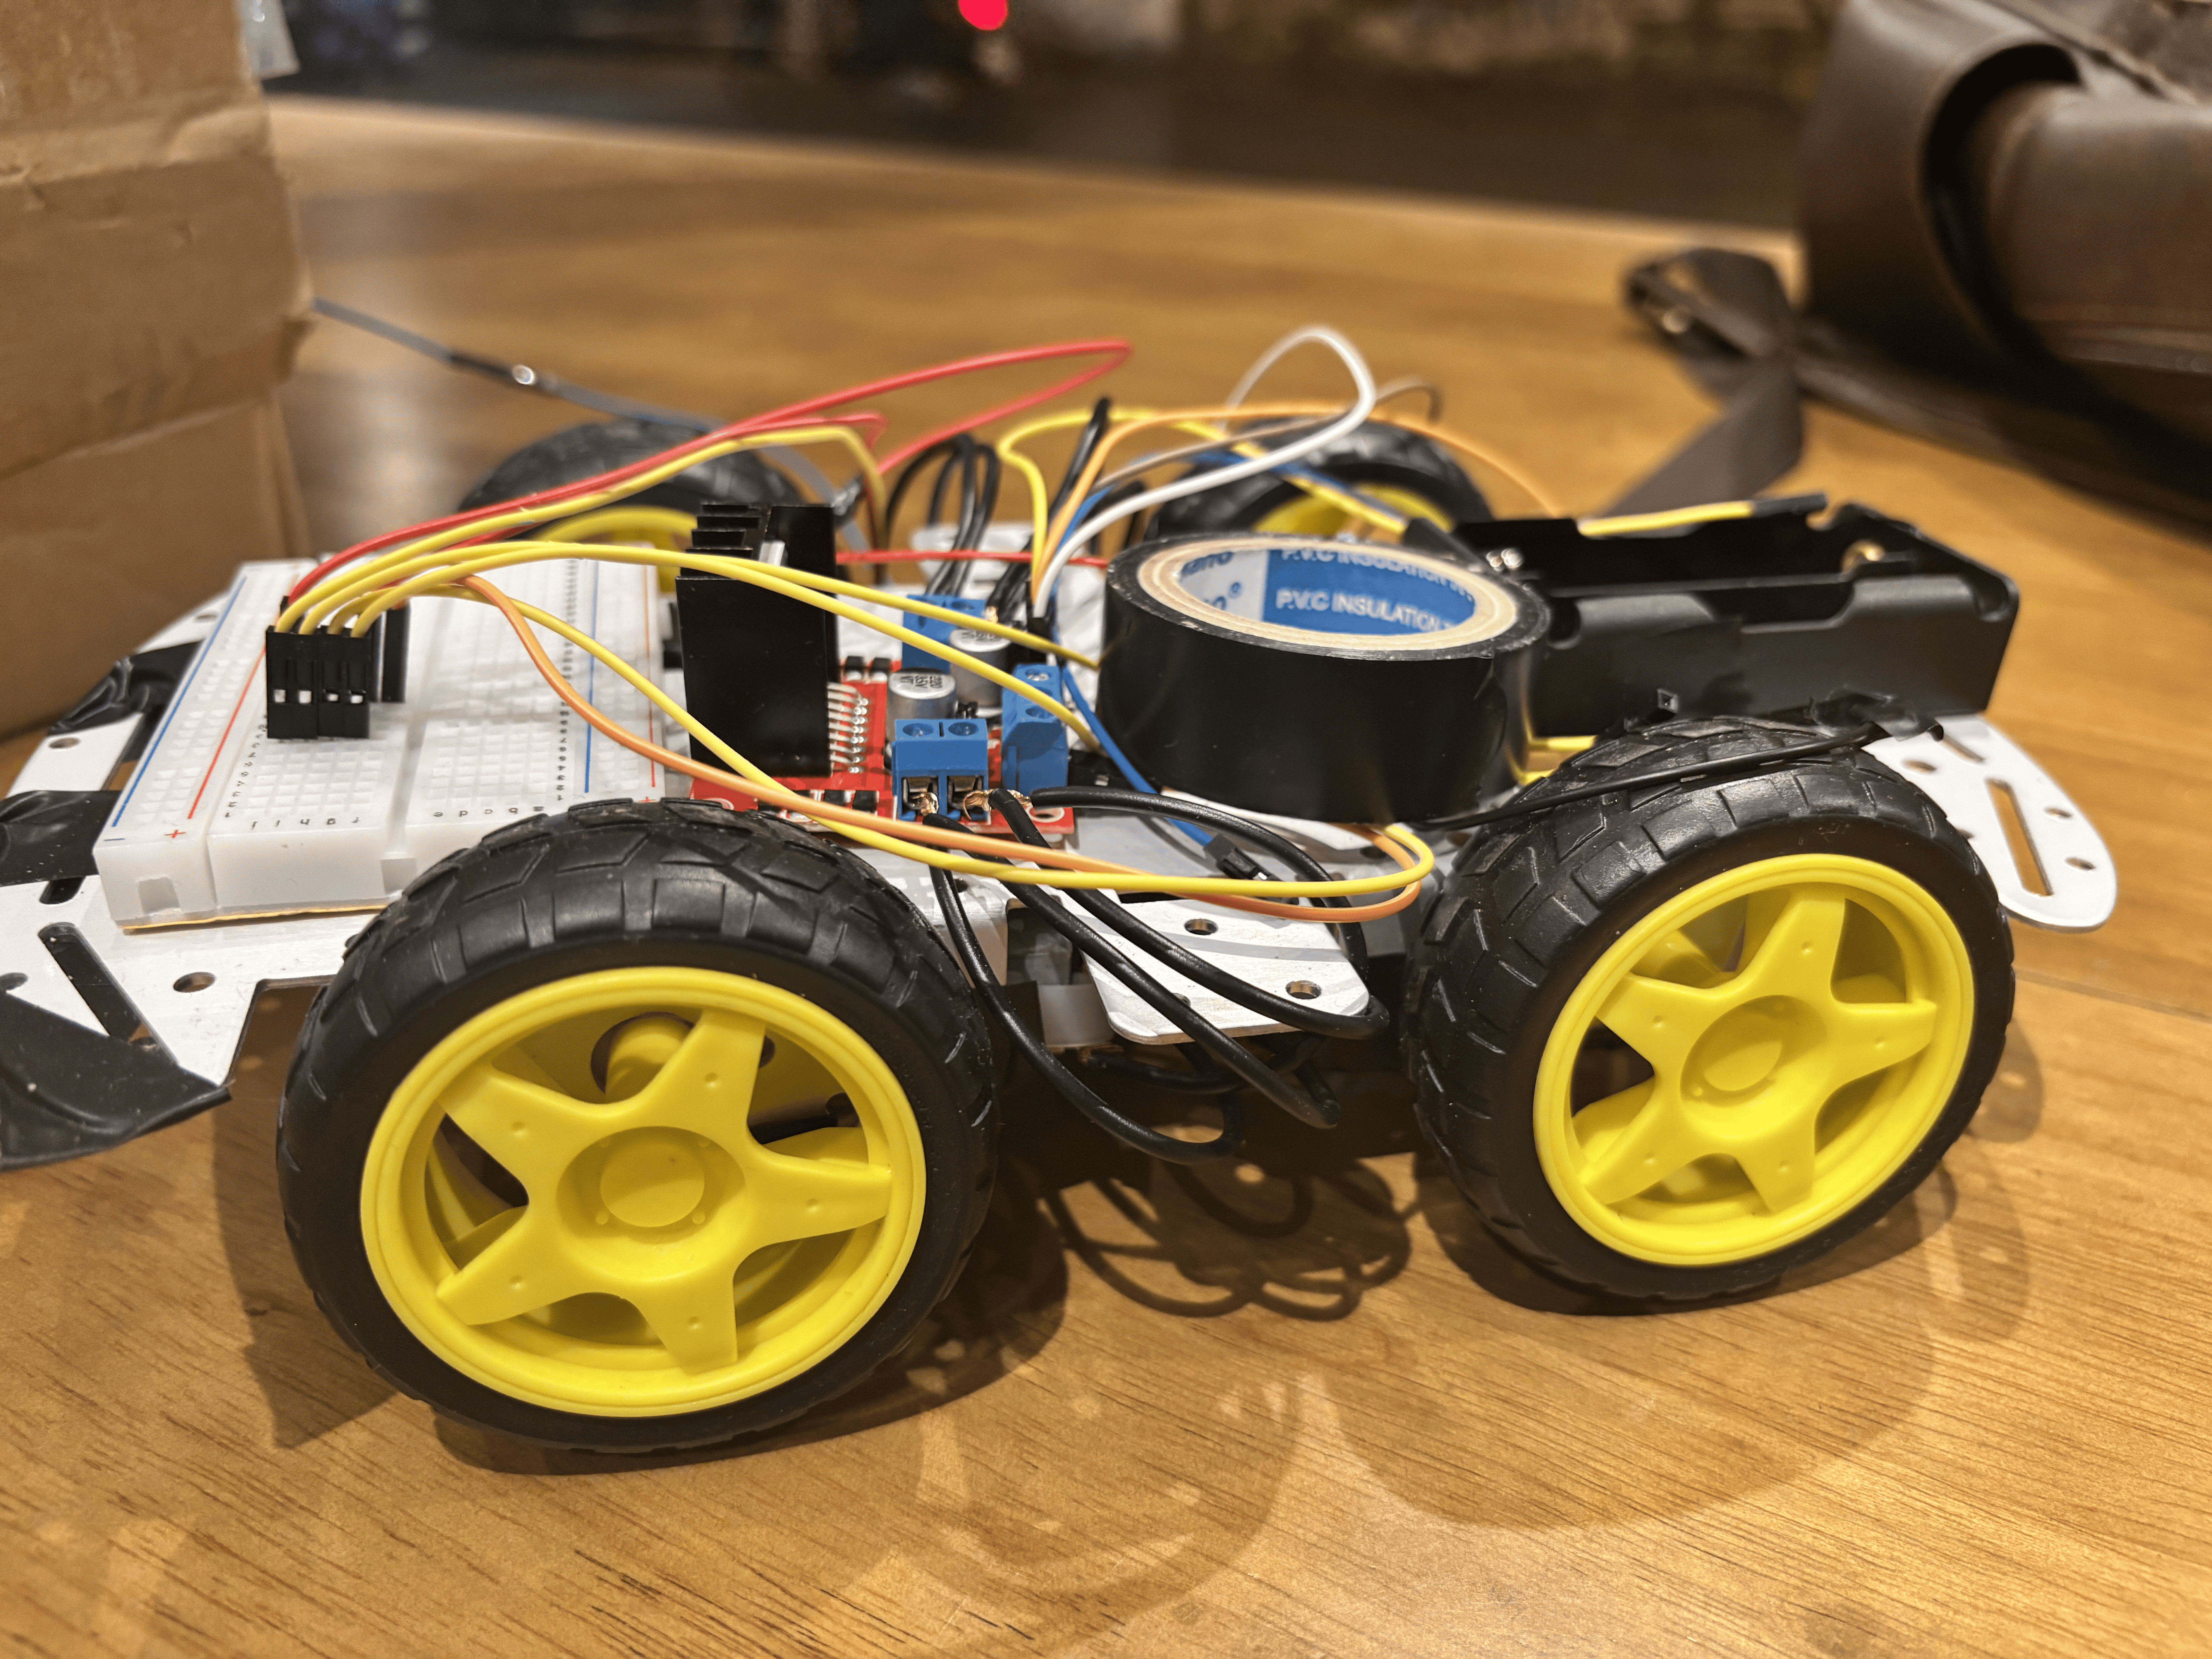
\includegraphics[width=\textwidth]{figures/hardware/rover_complete_photo.png}
    \caption{Fully assembled Rescue Rover showing the ESP32-S3 camera module, motor driver, battery, and chassis.}
    \label{fig:rover-complete}
\end{figure}

% --------------------------------------------------------
% SECTION 3.2: CHASSIS DESIGN
% --------------------------------------------------------
\section{Chassis Design}
\label{sec:chassis-design}

The chassis provides the structural foundation for all electronic components. We selected a commercially available \textbf{4-wheel drive (4WD)} chassis platform rather than designing a custom frame. This decision saved significant development time while providing a proven mechanical platform for the rover.

% SUBSECTION 3.2.1: PLATFORM SELECTION
\subsection{Platform Selection}

The selected chassis is a \textbf{dual-layer acrylic smart car platform}. Unlike the tracked tank-style alternatives initially considered, this wheeled design was chosen for its kinematic simplicity, higher top speed on flat surfaces, and easier maintenance. The acrylic construction allows for rapid modification and flexible component mounting.

\begin{table}[h!]
    \centering
    \caption{Chassis specifications (4WD Wheel Platform)}
    \label{tab:chassis-specs}
    \begin{tabular}{ll}
        \toprule
        \textbf{Parameter} & \textbf{Value} \\
        \midrule
        Drive System & 4-Wheel Drive (Independent DC Motors) \\
        Dimensions (L x W) & 255mm x 150mm (Chassis Plate) \\
        Full Width & $\approx$ 210mm (with wheels) \\
        Material & Laser-cut Acrylic \\
        Wheel Diameter & 65mm (Rubber tires) \\
        Motor Type & 1:48 Gear Ratio TT Motors \\
        \bottomrule
    \end{tabular}
\end{table}

% FIGURE 3.2: CHASSIS DIMENSIONS
% Placed inside Subsection 3.2.1
\begin{figure}[H]
    \centering
    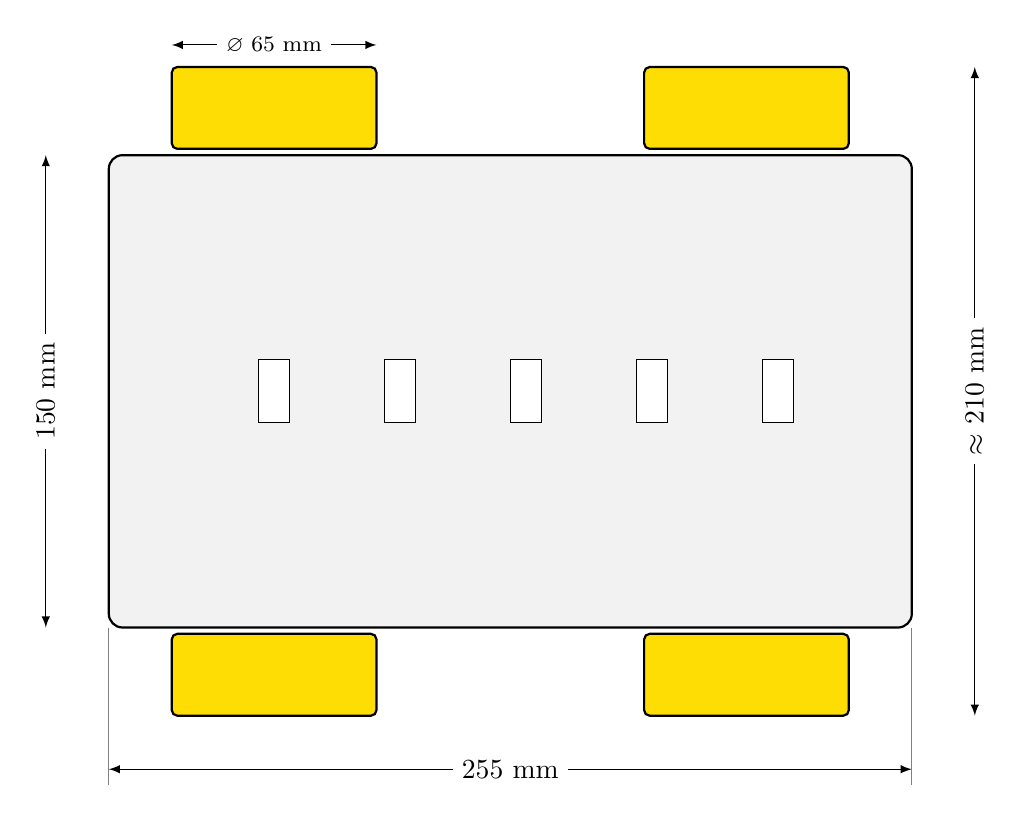
\begin{tikzpicture}[scale=0.04] 
        % Definitions
        \def\chassisL{255} 
        \def\chassisW{150} 
        \def\wheelL{65}    
        \def\wheelW{26}    

        % Styles
        \tikzstyle{dim} = [draw, <->, >=latex, thin, black]
        \tikzstyle{line} = [draw, thick, black]
        \tikzstyle{part} = [fill=gray!10, draw=black, thick]
        \tikzstyle{wheel} = [fill=yellow!80!orange, draw=black, thick, rounded corners=2pt]

        % Chassis
        \draw[part, rounded corners=5pt] (-\chassisL/2, -\chassisW/2) rectangle (\chassisL/2, \chassisW/2);
        \foreach \x in {-80, -40, 0, 40, 80} {
            \draw[fill=white] (\x, -10) rectangle (\x+10, 10);
        }

        % Wheels
        \draw[wheel] (-\chassisL/2 + 20, \chassisW/2 + 2) rectangle ++(\wheelL, \wheelW);
        \draw[wheel] (-\chassisL/2 + 20, -\chassisW/2 - 2 - \wheelW) rectangle ++(\wheelL, \wheelW);
        \draw[wheel] (\chassisL/2 - 20 - \wheelL, \chassisW/2 + 2) rectangle ++(\wheelL, \wheelW);
        \draw[wheel] (\chassisL/2 - 20 - \wheelL, -\chassisW/2 - 2 - \wheelW) rectangle ++(\wheelL, \wheelW);

        % Dimensions
        \draw[dim] (-\chassisL/2, -\chassisW/2 - 45) -- (\chassisL/2, -\chassisW/2 - 45) node[midway, fill=white] {255 mm};
        \draw[line, thin, gray] (-\chassisL/2, -\chassisW/2) -- (-\chassisL/2, -\chassisW/2 - 50);
        \draw[line, thin, gray] (\chassisL/2, -\chassisW/2) -- (\chassisL/2, -\chassisW/2 - 50);
        \draw[dim] (\chassisL/2 + 20, -\chassisW/2 - \wheelW - 2) -- (\chassisL/2 + 20, \chassisW/2 + \wheelW + 2) node[midway, fill=white, rotate=90] {$\approx$ 210 mm};
        \draw[dim] (-\chassisL/2 - 20, -\chassisW/2) -- (-\chassisL/2 - 20, \chassisW/2) node[midway, fill=white, rotate=90] {150 mm};
        \draw[dim] (-\chassisL/2 + 20, \chassisW/2 + 35) -- (-\chassisL/2 + 20 + \wheelL, \chassisW/2 + 35) node[midway, fill=white, font=\footnotesize] {$\varnothing$ 65 mm};

    \end{tikzpicture}
    \caption{Top-down dimensional schematic of the 4WD Rover chassis. The platform utilizes a double-layer acrylic frame with four independently driven DC geared motors.}
    \label{fig:chassis-dimensions}
\end{figure}

% SUBSECTION 3.2.2: WHEEL AND DRIVE ASSEMBLY
\subsection{Wheel and Drive Assembly}
\label{sec:drive-assembly}

Instead of the complex track tensioning system initially proposed, the rover utilizes a direct-drive configuration. Each of the four wheels is mounted directly to the output shaft of a DC gear motor. The system uses standard "TT" style motors with a 1:48 gear ratio. The wheels ($65\text{mm}$ diameter) feature a solid plastic rim with a rubber tire for traction. Torque is transferred via a double-flat mechanical interface that prevents the wheel from slipping on the motor shaft, eliminating the need for belts or tensioners.

% FIGURE 3.3: MOTOR DETAIL
% Placed inside Subsection 3.2.2
\begin{figure}[H]
    \centering
    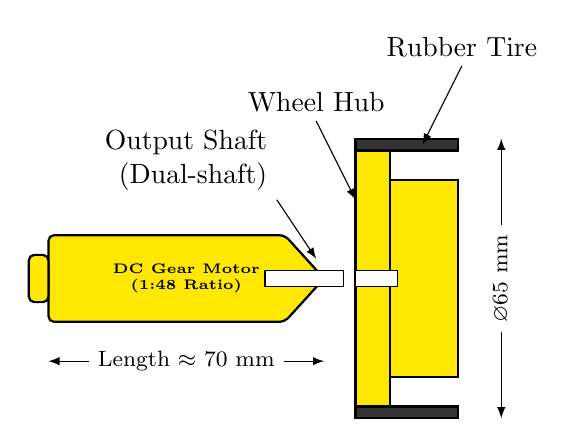
\begin{tikzpicture}[scale=0.05, >=latex]

        % Styles
        \tikzstyle{motor} = [draw=black, thick, fill=yellow!90!orange, rounded corners=2pt]
        \tikzstyle{tire} = [draw=black, fill=black!80, thick]
        \tikzstyle{rim} = [draw=black, fill=yellow!90!orange, thick]
        \tikzstyle{shaft} = [draw=black, fill=white]
        \tikzstyle{label} = [midway, fill=white, font=\footnotesize]
        \tikzstyle{dim} = [draw, <->, thin, black]

        % Definitions
        \def\motorL{70}
        \def\motorH{22}
        \def\wheelDia{65}
        \def\wheelW{26}

        % Drawing
        \draw[motor] (0, 0) -- (0, \motorH) -- (\motorL-10, \motorH) -- (\motorL, \motorH/2) -- (\motorL-10, 0) -- cycle;
        \draw[motor] (-5, 5) rectangle (0, \motorH-5);
        \node at (\motorL/2, \motorH/2) [font=\bfseries\tiny, align=center] {DC Gear Motor\\(1:48 Ratio)};

        \draw[shaft] (\motorL-15, \motorH/2 - 2) rectangle (\motorL+5, \motorH/2 + 2);

        \begin{scope}[shift={(\motorL+8, \motorH/2)}]
            \draw[tire] (0, \wheelDia/2) rectangle (\wheelW, \wheelDia/2 + 3); 
            \draw[tire] (0, -\wheelDia/2) rectangle (\wheelW, -\wheelDia/2 - 3); 
            \draw[rim] (0, -\wheelDia/2) rectangle (\wheelW/3, \wheelDia/2); 
            \draw[rim] (\wheelW/3, -25) rectangle (\wheelW, 25); 
            \draw[fill=white] (0, -2) rectangle (\wheelW/3 + 2, 2);
        \end{scope}

        % Dimensions
        \draw[dim] (\motorL+45, \motorH/2 - \wheelDia/2 - 3) -- (\motorL+45, \motorH/2 + \wheelDia/2 + 3) node[label, rotate=90] {$\varnothing 65$ mm};
        \draw[dim] (0, -10) -- (\motorL, -10) node[label] {Length $\approx$ 70 mm};

        % Annotations
        \draw[<-] (\motorL+8, \motorH/2 + 20) -- ++(-10, 20) node[anchor=south] {Wheel Hub};
        \draw[<-] (\motorL+25, \motorH/2 + 34) -- ++(10, 20) node[anchor=south] {Rubber Tire};
        \draw[<-] (\motorL-2, \motorH/2 + 5) -- ++(-10, 15) node[anchor=south east, align=right] {Output Shaft\\(Dual-shaft)};

    \end{tikzpicture}
    \caption{Drive assembly detail. The 1:48 ratio DC Gear Motor (left) couples directly to the 65mm wheel (right). The yellow plastic rim is press-fitted onto the motor output shaft.}
    \label{fig:drive-detail}
\end{figure}

\subsection{Component Mounting}
Electronic components are secured to the acrylic chassis to ensure stability during operation. The main PCB modules, such as the ESP32-S3 and the L298N motor driver, are mounted using \textbf{nylon standoffs and M3 screws}. This provides electrical isolation from the chassis and allows for easy removal. The prototyping breadboard is secured using a strong double-sided adhesive pad. Components are arranged longitudinally to distribute weight evenly between the front and rear axles, placing the heavier battery pack at the rear to counterbalance the camera and sensor array at the front.

% FIGURE PLACEHOLDER
\begin{figure}[H]
    \centering
    % FIX: Set x and y vectors to 1mm so "255" = 25.5cm, not 2.55 meters.
    % FIX: Scale 0.6 fits it nicely on a standard page width.
    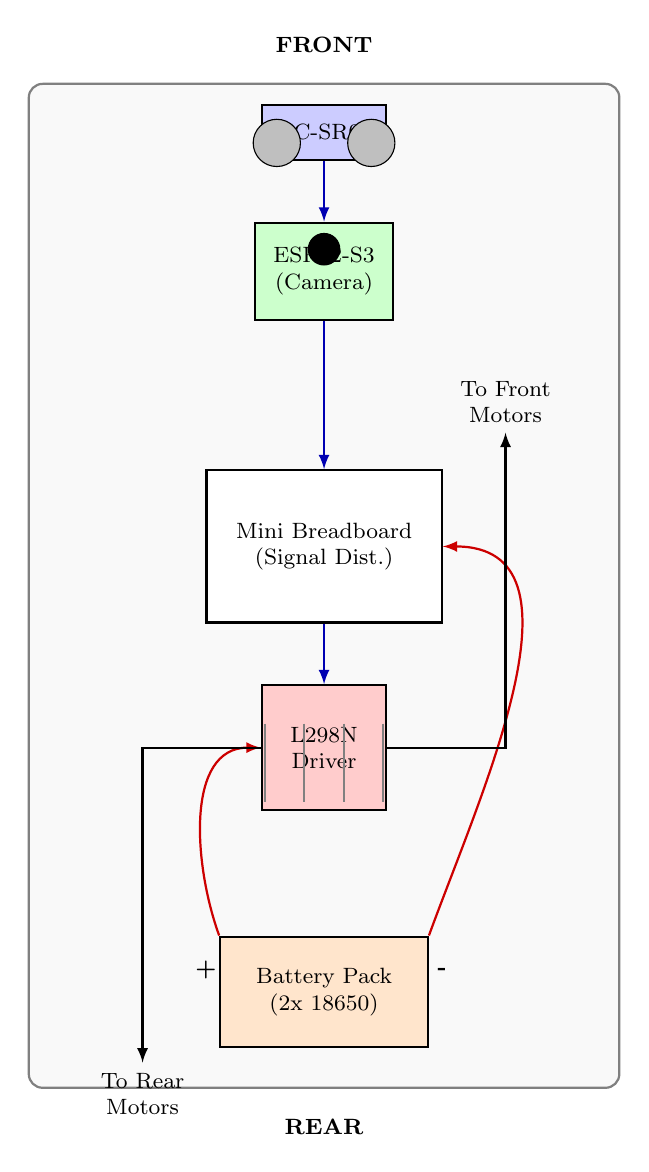
\begin{tikzpicture}[x=1mm, y=1mm, scale=0.5, >=latex, font=\footnotesize]

        % --- STYLES ---
        % FIX: Added 'align=center' to all nodes to allow line breaks (\\)
        \tikzstyle{chassis} = [draw=gray, thick, fill=gray!5, rounded corners=5pt]
        \tikzstyle{pcb_esp} = [draw=black, fill=green!20!white, thick, align=center]
        \tikzstyle{pcb_driver} = [draw=black, fill=red!20!white, thick, align=center]
        \tikzstyle{breadboard} = [draw=black, fill=white, thick, align=center] % Removed pattern to prevent errors
        \tikzstyle{sensor} = [draw=black, fill=blue!20!white, thick, align=center]
        \tikzstyle{battery} = [draw=black, fill=orange!20!white, thick, align=center]
        \tikzstyle{wire} = [draw=blue!70!black, thick, ->]
        \tikzstyle{label_node} = [fill=white, draw=black, thin, inner sep=2pt, align=center]

        % --- DEFINITIONS ---
        \def\cL{255} % Chassis Length (now interpreted as mm)
        \def\cW{150} % Chassis Width (now interpreted as mm)

        % --- CHASSIS BASE ---
        \draw[chassis] (-\cW/2, -\cL/2) rectangle (\cW/2, \cL/2);
        \node at (0, \cL/2 + 10) {\textbf{FRONT}};
        \node at (0, -\cL/2 - 10) {\textbf{REAR}};

        % --- COMPONENTS ---

        % 1. Ultrasonic Sensor (Front)
        \node[sensor, minimum width=45, minimum height=20, anchor=north] (us) at (0, \cL/2 - 5) {HC-SR04};
        % Add "eyes"
        \draw[fill=gray!50] (-12, \cL/2 - 15) circle (6);
        \draw[fill=gray!50] (12, \cL/2 - 15) circle (6);

        % 2. ESP32-S3 Camera Module (Behind sensor)
        \node[pcb_esp, minimum width=50, minimum height=35, anchor=north] (esp) at (0, \cL/2 - 35) {ESP32-S3\\(Camera)};
        % Add lens indication
        \draw[fill=black] (0, \cL/2 - 42) circle (4);

        % 3. Breadboard (Middle)
        \node[breadboard, minimum width=85, minimum height=55] (bb) at (0, 10) {Mini Breadboard\\(Signal Dist.)};

        % 4. L298N Motor Driver (Behind breadboard)
        \node[pcb_driver, minimum width=45, minimum height=45, anchor=north] (driver) at (0, -25) {L298N\\Driver};
        % Add heatsink graphic
        \foreach \x in {-15, -5, 5, 15} \draw[gray, thick] (\x, -35) -- (\x, -55);

        % 5. Battery Pack (Rear)
        \node[battery, minimum width=75, minimum height=40, anchor=south] (batt) at (0, -\cL/2 + 10) {Battery Pack\\(2x 18650)};
        % Add terminals
        \node at (-30, -\cL/2 + 30) {\textbf{+}};
        \node at (30, -\cL/2 + 30) {\textbf{-}};

        % --- LOGICAL CONNECTIONS (Schematic Wires) ---
        % Sensor to ESP
        \draw[wire] (us.south) -- (esp.north);
        % ESP to Breadboard
        \draw[wire] (esp.south) -- (bb.north);
        % Breadboard to Driver (Control signals)
        \draw[wire] (bb.south) -- (driver.north);
        
        % Battery to Driver (Power)
        % Note: Adjusted 'out' angle slightly to be smoother
        \draw[wire, draw=red!80!black] (batt.north west) to[out=110, in=180] (driver.west);
        
        % Battery to ESP (Power via regulator/breadboard)
        \draw[wire, draw=red!80!black] (batt.north east) to[out=70, in=0] (bb.east);

        % Motor outputs (schematic)
        \draw[wire, draw=black, thick] (driver.east) -- ++(30,0) -- ++(0, 80) node[above, align=center] {To Front\\Motors};
        \draw[wire, draw=black, thick] (driver.west) -- ++(-30,0) -- ++(0, -80) node[below, align=center] {To Rear\\Motors};

    \end{tikzpicture}
    \caption{Schematic top-down view of the component layout. The ultrasonic sensor and camera are positioned at the front for unobstructed sensing. The heavier battery pack is placed at the rear to balance the center of gravity. Power and signal lines are shown logically.}
    \label{fig:component-layout}
\end{figure}

% --------------------------------------------------------
\section{Main Controller: ESP32-S3}
\label{sec:esp32-controller}

The ESP32-S3 serves as the central processing unit for the rover. This chip was selected for its combination of processing power, wireless capabilities, camera interface, and extensive Arduino ecosystem support.

\subsection{Chip Specifications}

The ESP32-S3 is Espressif's third generation WiFi/Bluetooth microcontroller. It features dual Xtensa LX7 cores running at up to 240 MHz, significantly more powerful than the original ESP32.

\begin{table}[H]
    \centering
    \caption{ESP32-S3 technical specifications}
    \label{tab:esp32-specs}
    \begin{tabular}{ll}
        \toprule
        \textbf{Feature} & \textbf{Specification} \\
        \midrule
        CPU           & Dual Xtensa LX7, up to 240 MHz \\
        SRAM          & 512 KB internal \\
        PSRAM         & 8 MB external (OPI interface) \\
        Flash         & 16 MB (QSPI) \\
        WiFi          & 802.11 b/g/n, 2.4 GHz \\
        Bluetooth     & LE 5.0 with coded PHY \\
        GPIO          & 45 programmable pins \\
        Camera        & DVP interface, up to 2MP \\
        USB           & USB 2.0 OTG \\
        Operating voltage & 3.0-3.6V (LDO regulates from 5V)\\
        \bottomrule
    \end{tabular}
\end{table}

% FIGURE PLACEHOLDER
\begin{figure}[H]
    \centering
    \includegraphics[width=0.7\textwidth]{figures/hardware/esp32s3_module_photo.jpeg}
    \caption{ESP32-S3 WROOM development board used in the Rescue Rover.}
    \label{fig:esp32-module}
\end{figure}

\subsection{Development Board Selection}

Several ESP32-S3 development boards were evaluated. The Freenove ESP32-S3 WROOM was selected for its integrated camera connector, adequate PSRAM, and reasonable price point. Other options considered included the official Espressif DevKitC and the AI-Thinker ESP32-S3 CAM.

\begin{table}[H]
    \centering
    \caption{ESP32-S3 development board comparison}
    \label{tab:board-comparison}
    \begin{tabular}{lccc}
        \toprule
        \textbf{Feature} & \textbf{Freenove} & \textbf{ESP32-CAM} & \textbf{DevKitC} \\
        \midrule
        PSRAM             & 8 MB  & 4 MB  & 8 MB \\
        Camera connector  & Yes   & Yes   & No \\
        Available GPIO    & 35+   & 10    & 45 \\
        USB programming   & Built-in & External & Built-in \\
        Price             & \$12  & \$8   & \$15 \\
        Selected          & Yes   & No    & No \\
        \bottomrule
    \end{tabular}
\end{table}

The ESP32-CAM was rejected despite its lower cost because of severe GPIO limitations. Many pins are shared between the camera, SD card, and flash, leaving insufficient pins for motor control and sensors.

% FIGURE PLACEHOLDER
% FIGURE: BOARD COMPARISON
\begin{figure}[H]
    \centering
    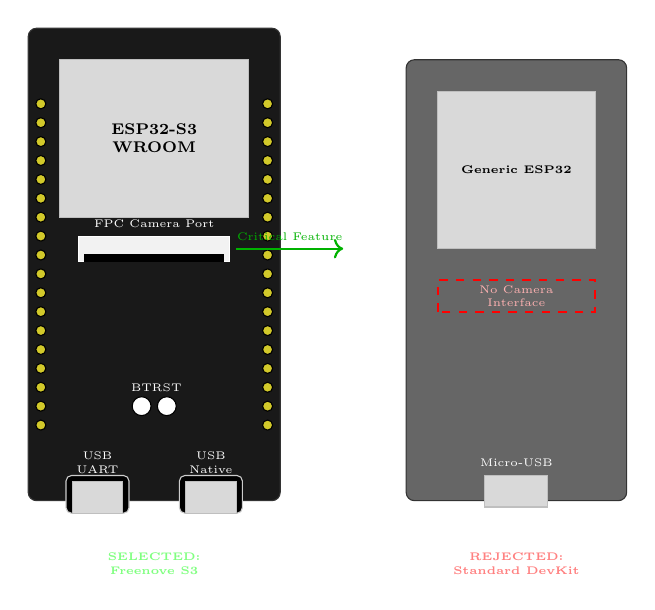
\begin{tikzpicture}[scale=0.8, transform shape, font=\sffamily\footnotesize]

        % Styles
        \tikzstyle{pcb} = [draw=black!80, fill=black!90, rounded corners=3pt]
        \tikzstyle{metal} = [draw=gray!50, fill=gray!30]
        \tikzstyle{conn} = [draw=white, fill=white!90!gray]
        \tikzstyle{usbc} = [draw=gray!40, fill=black, rounded corners=2pt]
        \tikzstyle{label} = [text=white, font=\bfseries\tiny, align=center]
        
        % --- LEFT: FREENOVE S3 (SELECTED) ---
        \begin{scope}[shift={(0,0)}]
            % PCB Outline
            \draw[pcb] (0,0) rectangle (4.0, 7.5);
            
            % ESP32-S3 Module
            \draw[metal] (0.5, 4.5) rectangle (3.5, 7.0);
            \node[text=black, font=\bfseries\scriptsize, align=center] at (2.0, 5.75) {ESP32-S3\\WROOM};

            % FPC Camera Connector (The distinctive white bar)
            \draw[conn] (0.8, 3.8) rectangle (3.2, 4.2);
            \draw[black, fill=black] (0.9, 3.8) rectangle (3.1, 3.9); % Latch
            \node[text=white, font=\tiny] at (2.0, 4.4) {FPC Camera Port};

            % Dual USB-C Ports (Bottom)
            \draw[usbc] (0.6, -0.2) rectangle (1.6, 0.4); % UART
            \draw[metal] (0.7, -0.2) rectangle (1.5, 0.3); % Metal casing
            \node[text=white, font=\tiny, align=center] at (1.1, 0.6) {USB\\UART};

            \draw[usbc] (2.4, -0.2) rectangle (3.4, 0.4); % OTG
            \draw[metal] (2.5, -0.2) rectangle (3.3, 0.3); % Metal casing
            \node[text=white, font=\tiny, align=center] at (2.9, 0.6) {USB\\Native};

            % Header Pins
            \foreach \y in {1.2, 1.5, ..., 6.5} {
                \draw[fill=yellow!80!black] (0.2, \y) circle (0.08);
                \draw[fill=yellow!80!black] (3.8, \y) circle (0.08);
            }

            % Buttons (Boot/Rst)
            \draw[fill=white] (1.8, 1.5) circle (0.15); \node[text=white, font=\tiny] at (1.8, 1.8) {BT};
            \draw[fill=white] (2.2, 1.5) circle (0.15); \node[text=white, font=\tiny] at (2.2, 1.8) {RST};

            % Label
            \node[label, text=green!50] at (2.0, -1.0) {SELECTED:\\Freenove S3};
        \end{scope}

        % --- RIGHT: STANDARD DEVKIT (REJECTED) ---
        \begin{scope}[shift={(6,0)}]
            % PCB Outline
            \draw[pcb, fill=black!60] (0,0) rectangle (3.5, 7.0);
            
            % Module
            \draw[metal] (0.5, 4.0) rectangle (3.0, 6.5);
            \node[text=black, font=\bfseries\tiny] at (1.75, 5.25) {Generic ESP32};

            % NO Camera Port (Crossed out area)
            \draw[red, dashed, thick] (0.5, 3.0) rectangle (3.0, 3.5);
            \node[text=red!30, font=\tiny, align=center] at (1.75, 3.25) {No Camera\\Interface};

            % Single Micro-USB
            \draw[metal] (1.25, -0.1) rectangle (2.25, 0.4);
            \node[text=white, font=\tiny] at (1.75, 0.6) {Micro-USB};

            % Label
            \node[label, text=red!50] at (1.75, -1.0) {REJECTED:\\Standard DevKit};
        \end{scope}

        % --- COMPARISON ARROWS ---
        \draw[->, thick, green!70!black] (3.3, 4.0) -- (5.0, 4.0) node[midway, above, font=\tiny] {Critical Feature};

    \end{tikzpicture}
    \caption{Comparison of development boards. The Freenove S3 (left) was selected for its dedicated FPC camera connector and dual USB-C interfaces, features absent on standard development boards (right).}
    \label{fig:board-comparison}
\end{figure}

\subsection{PSRAM Importance}

External PSRAM is essential for camera operation. Each QVGA frame requires 153.6 KB of buffer space. Double buffering doubles this requirement. Without PSRAM, the internal 512 KB SRAM would be exhausted by camera buffers alone, leaving no memory for the application.

The PSRAM connects via OPI (Octal Peripheral Interface) rather than QPI (Quad). OPI provides higher bandwidth, supporting faster frame transfers from the camera peripheral to the CPU.

% --------------------------------------------------------
\section{Camera System}
\label{sec:camera-hardware}

The camera provides the rover's primary sensing capability. Visual data is used for remote operation, obstacle detection, and AI scene analysis.

\subsection{OV2640 Sensor}

The OV2640 is a 2-megapixel CMOS image sensor commonly used in embedded vision applications. It connects to the ESP32-S3 through the DVP (Digital Video Port) parallel interface.

\begin{table}[h!]
    \centering
    \caption{OV2640 camera sensor specifications}
    \label{tab:ov2640-specs}
    \begin{tabular}{ll}
        \toprule
        \textbf{Parameter} & \textbf{Value} \\
        \midrule
        Resolution (max)   & 1600 x 1200 (2 MP) \\
        Output formats     & JPEG, YUV422, RGB565 \\
        Frame rate (SVGA)  & 30 FPS \\
        Frame rate (UXGA)  & 15 FPS \\
        Interface          & DVP (8-bit parallel) \\
        Control bus        & I2C (SCCB compatible) \\
        Operating voltage  & 2.5V core, 2.8V I/O \\
        Active pixels      & 1632 x 1232 \\
        Pixel size         & 2.2 x 2.2 $\mu$m \\
        \bottomrule
    \end{tabular}
\end{table}

% FIGURE PLACEHOLDER
\begin{figure}[h!]
    \centering
    \includegraphics[width=0.5\textwidth]{figures/hardware/ov2640_module.jpeg}
    \caption{OV2640 camera module showing the lens assembly and 24-pin FPC connector.}
    \label{fig:ov2640-module}
\end{figure}

\subsection{Resolution Selection}
The firmware configures the OV2640 sensor for **QVGA ($320 \times 240$)** resolution. This specific setting was chosen as the optimal trade-off point. While the sensor supports up to UXGA ($1600 \times 1200$), resolutions above QVGA generate JPEG payloads that exceed the standard Ethernet MTU (1500 bytes), requiring complex UDP packet fragmentation and reassembly which increases latency.

\begin{table}[h!]
    \centering
    \caption{Resolution bandwidth trade-offs (OV2640 JPEG)}
    \label{tab:resolution-tradeoffs}
    \begin{tabular}{lcccc}
        \toprule
        \textbf{Resolution} & \textbf{Pixel Count} & \textbf{Avg Frame Size} & \textbf{UDP Efficiency} & \textbf{Status} \\
        \midrule
        QQVGA ($160\times120$) & 19,200    & 2-4 KB   & High (1 pkt) & Rejected (Low Detail) \\
        \textbf{QVGA ($320\times240$)}  & \textbf{76,800}    & \textbf{6-12 KB}  & \textbf{Medium (4-8 pkts)} & \textbf{Selected} \\
        VGA ($640\times480$)   & 307,200   & 25-40 KB & Low (20+ pkts)  & Rejected (High Latency) \\
        SVGA ($800\times600$)  & 480,000   & 50-80 KB & Very Low  & Rejected \\
        \bottomrule
    \end{tabular}
\end{table}

% FIGURE: RESOLUTION COMPARISON
\begin{figure}[h!]
    \centering
    % FIX: Set x and y to 0.2mm. 640 * 0.2mm = 128mm (12.8cm), which fits on the page.
    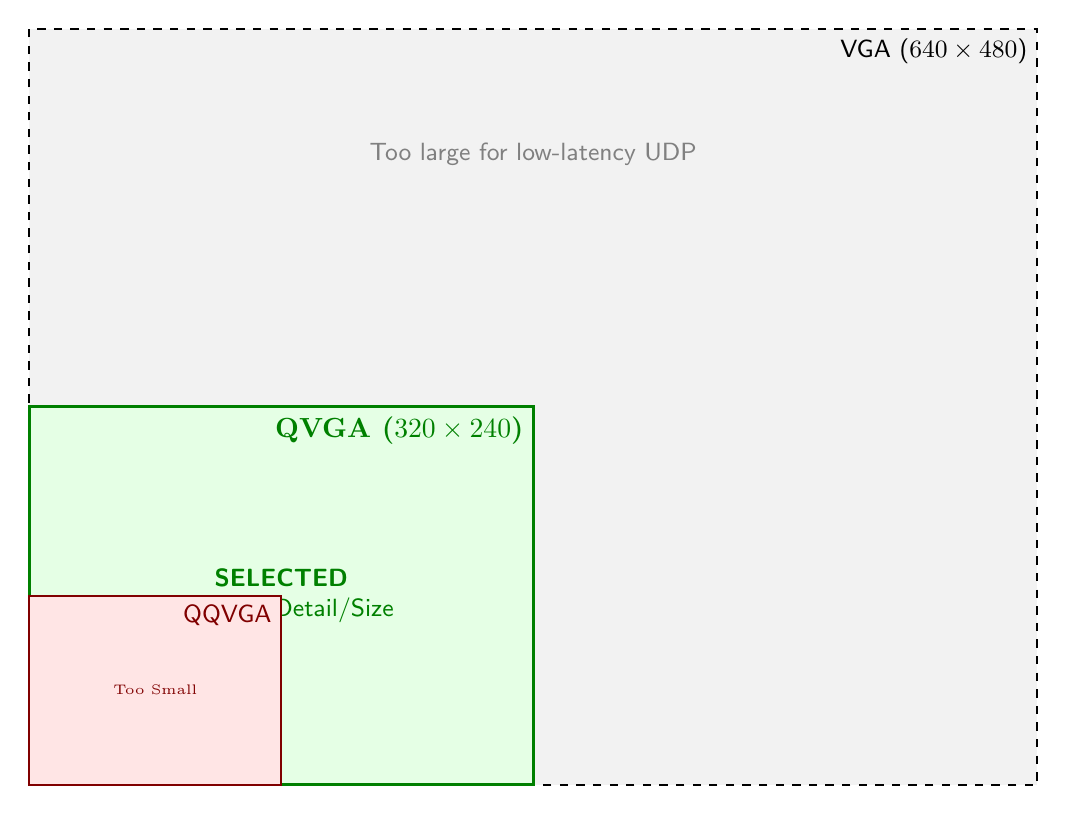
\begin{tikzpicture}[x=0.2mm, y=0.2mm, font=\sffamily\small]
        
        % Styles
        \tikzstyle{frame} = [draw=black, thick, fill=blue!5]
        \tikzstyle{label} = [fill=white, inner sep=2pt, draw=black!50]

        % VGA Frame (Reference Background)
        \draw[frame, fill=gray!10, dashed] (0,0) rectangle (640, 480);
        \node[anchor=north east] at (640, 480) {VGA ($640 \times 480$)};
        \node at (320, 400) [text=gray] {Too large for low-latency UDP};

        % QVGA Frame (Selected)
        \draw[frame, fill=green!10, draw=green!50!black, very thick] (0,0) rectangle (320, 240);
        \node[anchor=north east, text=green!50!black, font=\bfseries] at (320, 240) {QVGA ($320 \times 240$)};
        \node[align=center, text=green!50!black] at (160, 120) {\textbf{SELECTED}\\Balanced Detail/Size};

        % QQVGA Frame (Too Small)
        \draw[frame, fill=red!10, draw=red!50!black] (0,0) rectangle (160, 120);
        \node[anchor=north east, text=red!50!black] at (160, 120) {QQVGA};
        \node[text=red!50!black, font=\tiny] at (80, 60) {Too Small};

    \end{tikzpicture}
    \caption{Relative frame size comparison. The selected QVGA resolution (green) offers 4x the pixel data of QQVGA while remaining significantly smaller than VGA, fitting within the bandwidth constraints of the ESP32.}
    \label{fig:resolution-comparison}
\end{figure}

\subsection{Lens and Optical Configuration}
The system utilizes the standard lens provided with the OV2640 module. This lens features a **$65^\circ$ horizontal field of view (FOV)**. While narrower than fisheye alternatives ($120^\circ+$), this standard lens provides rectilinear images with minimal distortion, simplifying the object detection algorithms. The blind spot immediately in front of the bumper is compensated for by the downward tilt of the mounting bracket.

% FIGURE: FOV DIAGRAM
\begin{figure}[h!]
    \centering
    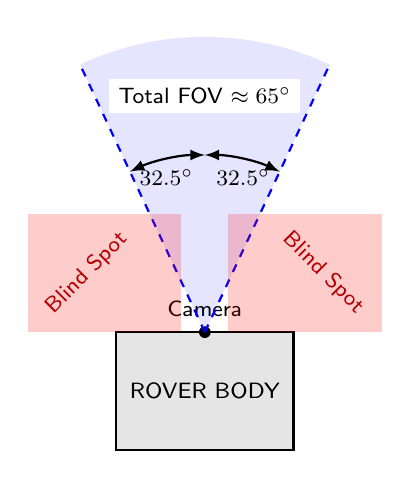
\begin{tikzpicture}[scale=0.15, >=latex, font=\sffamily\footnotesize]

        % Rover Body (Top View)
        \draw[fill=gray!20, draw=black, thick] (-7.5, -10) rectangle (7.5, 0);
        \node at (0, -5) {ROVER BODY};
        
        % Camera Position
        \node[circle, fill=black, inner sep=1.5pt] (cam) at (0, 0) {};
        \node[above] at (0,0.5) {Camera};

        % FOV Cone (65 degrees)
        \draw[blue, thick, dashed] (0,0) -- (65:25);
        \draw[blue, thick, dashed] (0,0) -- (115:25);
        
        % Fill visible area
        \fill[blue, opacity=0.1] (0,0) -- (65:25) arc (65:115:25) -- cycle;

        % Labels
        \draw[<->, thick] (0, 15) arc (90:65:15) node[midway, below] {$32.5^\circ$};
        \draw[<->, thick] (0, 15) arc (90:115:15) node[midway, below] {$32.5^\circ$};
        \node[fill=white] at (0, 20) {Total FOV $\approx 65^\circ$};

        % Blind Spots
        \fill[red, opacity=0.2] (-15,0) rectangle (-2, 10);
        \node[red!70!black, rotate=45] at (-10, 5) {Blind Spot};
        
        \fill[red, opacity=0.2] (15,0) rectangle (2, 10);
        \node[red!70!black, rotate=-45] at (10, 5) {Blind Spot};

    \end{tikzpicture}
    \caption{Field of View (FOV) coverage diagram. The standard lens provides a $65^\circ$ viewing cone. Areas outside this cone (red) are blind spots requiring the rover to rotate for full situational awareness.}
    \label{fig:camera-fov}
\end{figure}

\subsection{Camera Mounting}
The camera module is secured to the front chassis using a custom 3D-printed bracket. The mount is designed with a fixed **$15^\circ$ downward tilt**. This angle ensures that the ground is visible starting approximately $10\text{cm}$ from the front bumper, allowing the rover to detect small obstacles on the floor while maintaining visibility of the horizon.

% FIGURE: MOUNTING SIDE VIEW
\begin{figure}[h!]
    \centering
    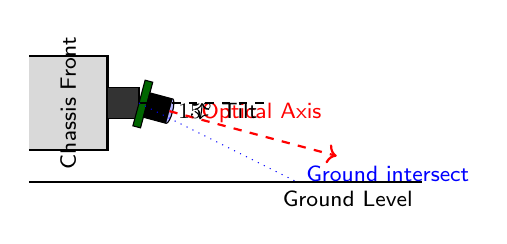
\begin{tikzpicture}[scale=0.2, font=\sffamily\footnotesize]

        % Ground
        \draw[thick] (-5, 0) -- (20, 0);
        \node[anchor=north east] at (20,0) {Ground Level};

        % Chassis Front
        \draw[fill=gray!30, draw=black, thick] (-5, 2) -- (0, 2) -- (0, 8) -- (-5, 8);
        \node[rotate=90] at (-2.5, 5) {Chassis Front};

        % Bracket
        \draw[fill=black!80] (0, 6) -- (2, 6) -- (2, 4) -- (0, 4) -- cycle;
        
        % Camera Module (Side Profile) - Tilted 15 degrees down
        % Pivot point at (2, 5)
        \begin{scope}[rotate around={-15:(2,5)}]
            % PCB
            \draw[fill=green!40!black] (2, 3.5) rectangle (2.5, 6.5);
            % Lens Barrel
            \draw[fill=black] (2.5, 4.2) rectangle (4.0, 5.8);
            % Lens Element
            \draw[fill=blue!30] (4.0, 4.2) arc (-90:90:0.2 and 0.8);
            
            % Optical Axis
            \draw[red, dashed, thick, ->] (4.0, 5) -- (15, 5);
            \node[red, above] at (10, 5.2) {Optical Axis};
        \end{scope}

        % Angle Indicator
        \draw[dashed] (2, 5) -- (10, 5); % Horizontal
        \draw[<->] (6, 5) arc (0:-15:4);
        \node at (7, 4.5) {$15^\circ$ Tilt};

        % Field of View Lines (Vertical)
        \draw[blue, dotted] (2,5) -- (12, 0); % Lower ray
        \node[blue, right] at (12, 0.5) {Ground intersect};

    \end{tikzpicture}
    \caption{Side-profile schematic of the camera mounting. The $15^\circ$ downward tilt aligns the optical axis to cover the floor surface ahead of the rover, eliminating the "under-nose" blind spot.}
    \label{fig:camera-mount}
\end{figure}

% --------------------------------------------------------
\section{Motor Control System}
\label{sec:motor-system}

The motor system provides locomotive power through two DC gear motors, one for each track. The L298N dual H-bridge driver controls motor direction and speed based on commands from the ESP32-S3.

\subsection{DC Gear Motors}

The motors are brushed DC type with integrated planetary gearboxes. The gearbox reduces output speed while increasing torque, essential for moving the chassis against friction and over obstacles.

\begin{table}[h!]
    \centering
    \caption{Motor specifications}
    \label{tab:motor-specs}
    \begin{tabular}{ll}
        \toprule
        \textbf{Parameter} & \textbf{Value} \\
        \midrule
        Nominal voltage    & 6-12V DC \\
        No-load speed      & 150 RPM at 12V \\
        Stall torque       & 3 kg-cm \\
        Stall current      & 1.5 A \\
        Operating current  & 200-500 mA \\
        Gear ratio         & 1:48 \\
        Shaft diameter     & 6 mm (D-cut) \\
        \bottomrule
    \end{tabular}
\end{table}

% FIGURE PLACEHOLDER
\begin{figure}[h!]
    \centering
    % \includegraphics[width=0.5\textwidth]{figures/hardware/dc_motor_gearbox.jpeg}
    \caption{DC gear motor showing the motor body, planetary gearbox, and output shaft.}
    \label{fig:motor-photo}
\end{figure}

\subsection{L298N Motor Driver}

The L298N is a dual full-bridge driver IC. Each bridge can deliver up to 2A continuous current, sufficient for our motors which draw 500mA under load. The module includes an onboard 5V regulator that powers the ESP32-S3.

\begin{table}[h!]
    \centering
    \caption{L298N specifications}
    \label{tab:l298n-specs}
    \begin{tabular}{ll}
        \toprule
        \textbf{Parameter} & \textbf{Value} \\
        \midrule
        Motor supply voltage & 5-35V \\
        Logic supply         & 5V (from onboard regulator or external) \\
        Per channel current  & 2A continuous, 3A peak \\
        Total power          & 25W max \\
        Control inputs       & 4 (IN1-IN4) \\
        Enable inputs        & 2 (ENA, ENB) \\
        Voltage drop         & 1.8V typical (at rated current) \\
        \bottomrule
    \end{tabular}
\end{table}

% FIGURE PLACEHOLDER
\begin{figure}[h!]
    \centering
    \includegraphics[width=0.6\textwidth]{figures/hardware/l298n_module.jpeg}
    \caption{L298N motor driver module with the characteristic large heatsink and terminal blocks.}
    \label{fig:l298n-module}
\end{figure}

\subsection{L298N vs TB6612FNG}

During component selection, we compared the L298N against the more modern TB6612FNG. The TB6612 offers higher efficiency (90\% vs 70\%) due to MOSFET switching rather than bipolar transistors. However, the L298N was selected because of its higher current capacity and integrated voltage regulator.

\begin{table}[h!]
    \centering
    \caption{Motor driver comparison}
    \label{tab:driver-comparison}
    \begin{tabular}{lcc}
        \toprule
        \textbf{Feature} & \textbf{L298N} & \textbf{TB6612FNG} \\
        \midrule
        Max current     & 2A    & 1.2A \\
        Efficiency      & 70\%  & 90\% \\
        Voltage drop    & 1.8V  & 0.3V \\
        Heat generation & High  & Low \\
        5V regulator    & Built-in & None \\
        Cost            & \$3   & \$5 \\
        Selected        & Yes   & No \\
        \bottomrule
    \end{tabular}
\end{table}

The lower efficiency of the L298N means more power is dissipated as heat. For extended operation, the heatsink temperature can exceed 60 degrees Celsius. Future revisions may switch to the TB6612 if thermal throttling becomes problematic.

% FIGURE PLACEHOLDER
\begin{figure}[h!]
    \centering
    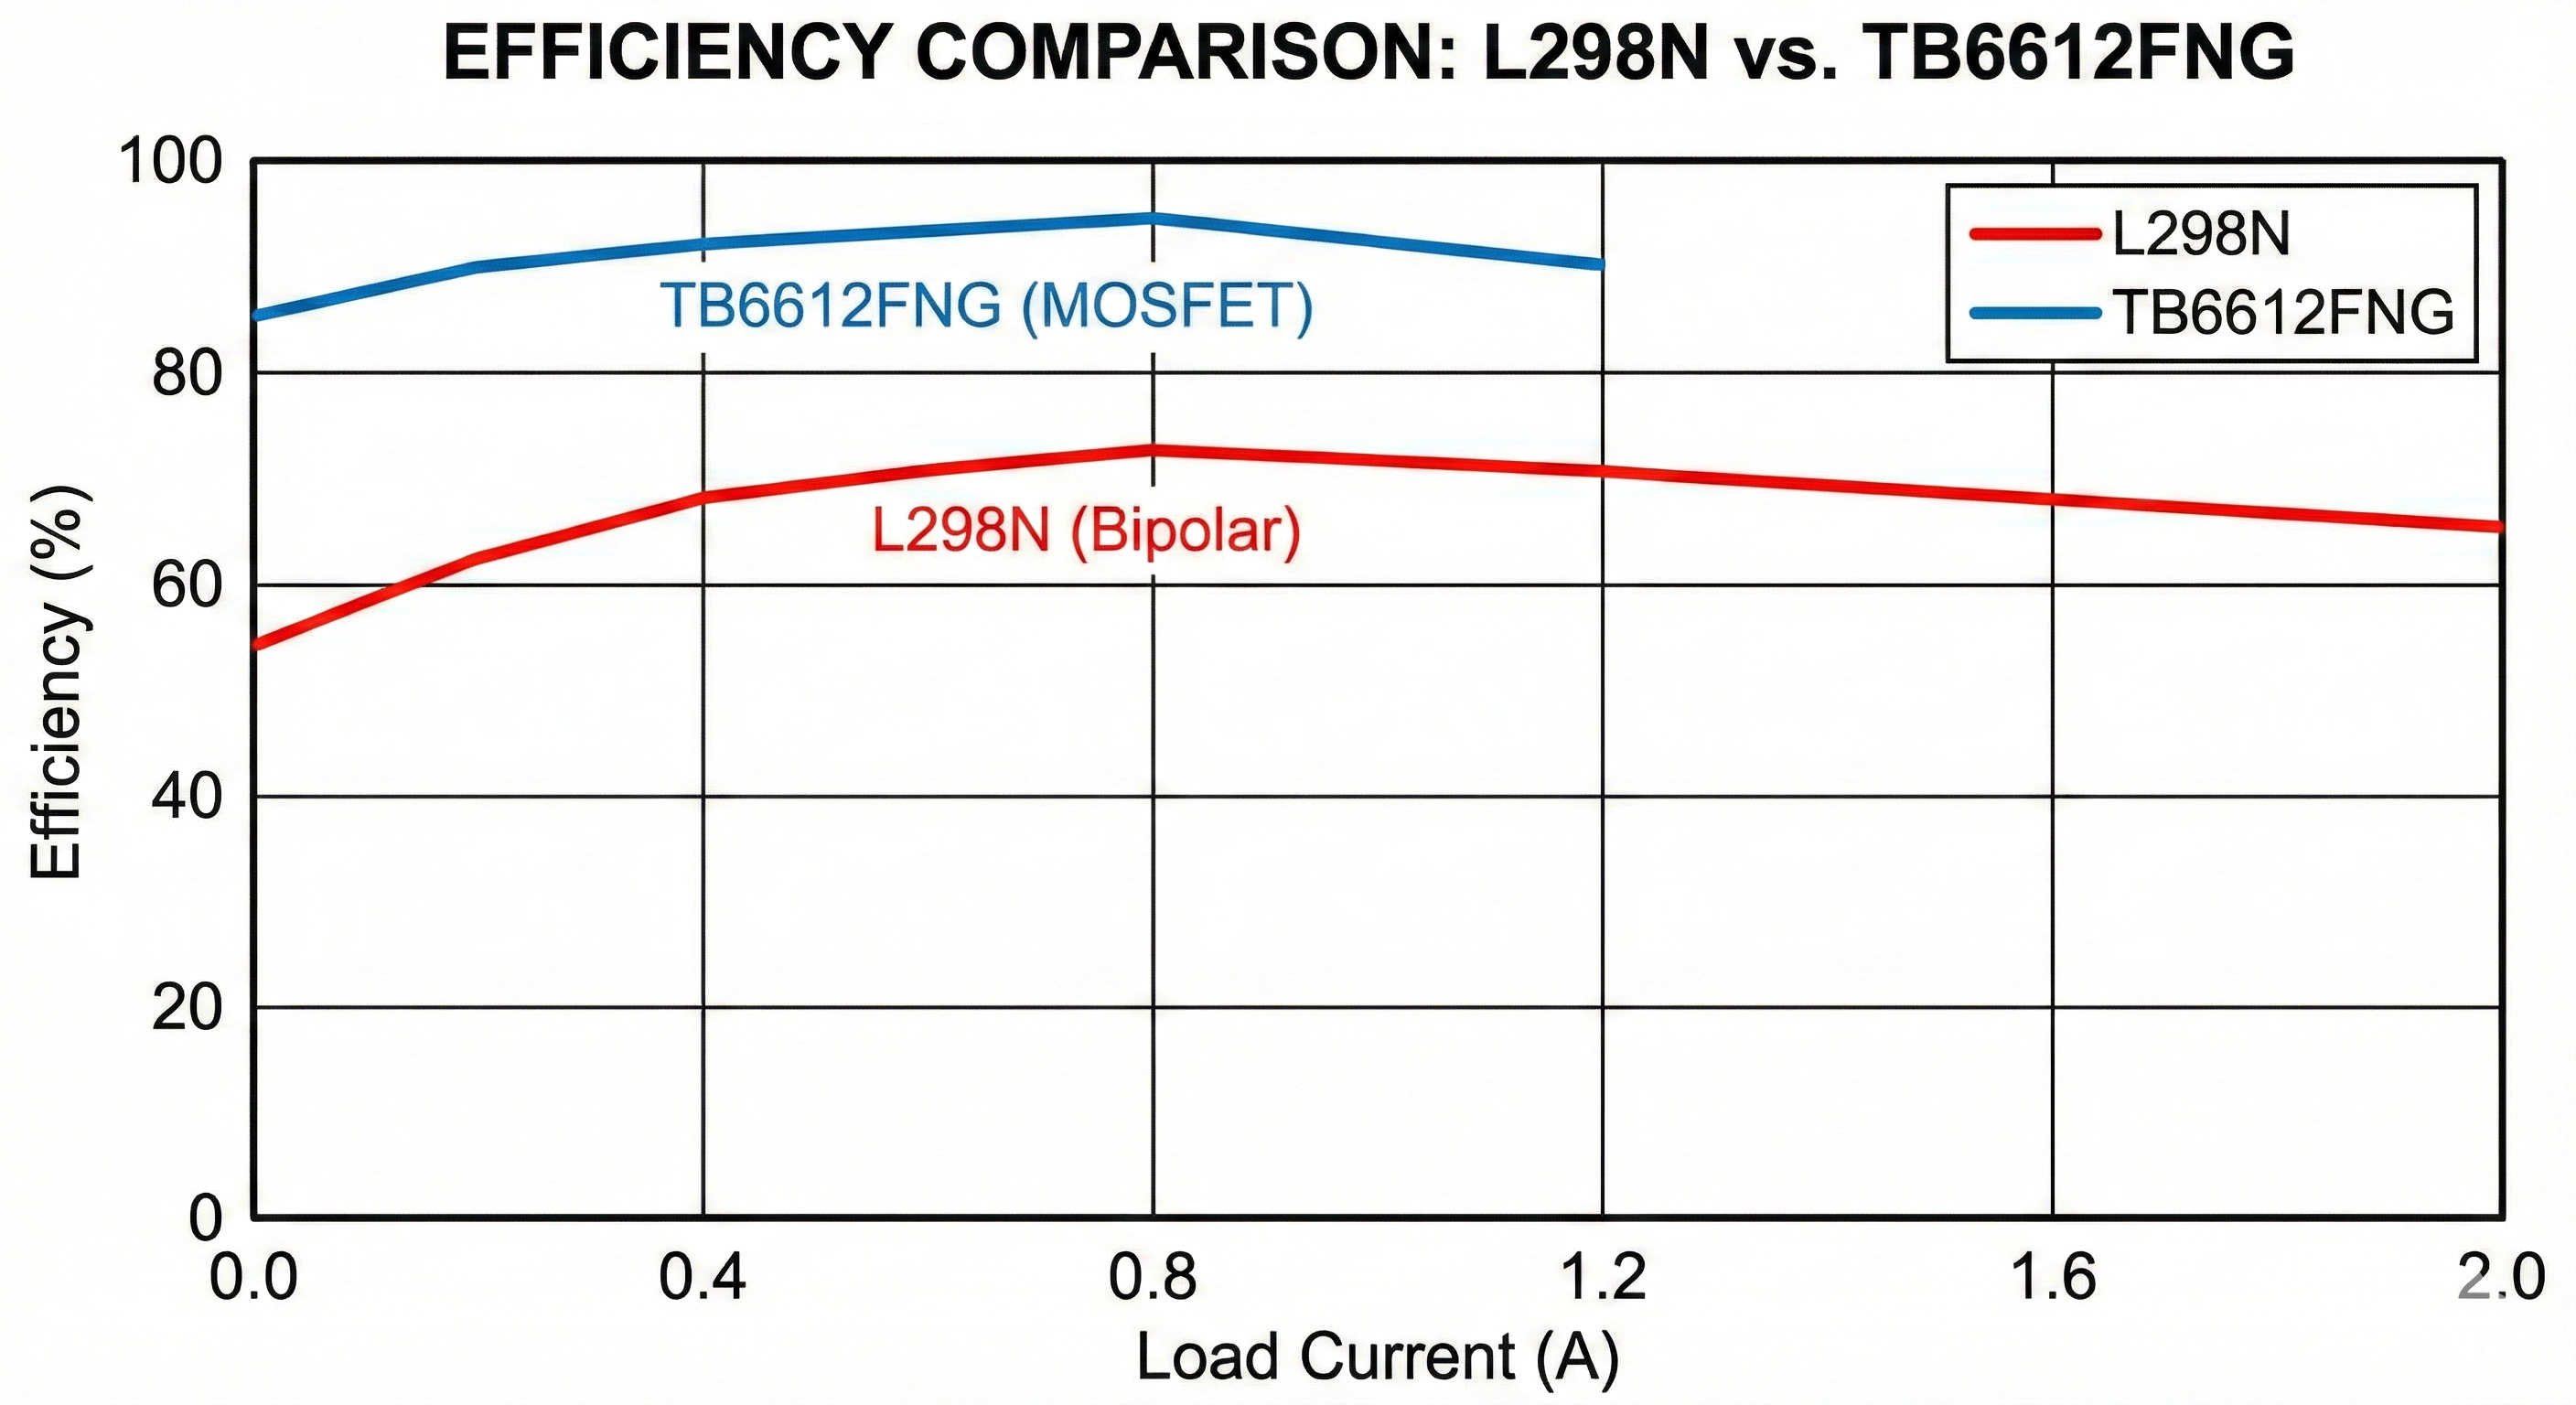
\includegraphics[width=0.8\textwidth]{figures/charts/driver_efficiency.png}
    \label{fig:efficiency-graph}
\end{figure}

% --------------------------------------------------------
\section{Power Distribution}
\label{sec:power-distribution}

The power system delivers appropriate voltages to all components from a single lithium polymer battery. Power management includes voltage regulation, protection circuits, and monitoring.

\subsection{Battery Selection}

A 3-cell (3S) lithium polymer battery provides the primary power. The 11.1V nominal voltage is compatible with both the motors (rated for 6-12V) and the L298N 5V regulator input range.

\begin{table}[h!]
    \centering
    \caption{Battery specifications}
    \label{tab:battery-specs}
    \begin{tabular}{ll}
        \toprule
        \textbf{Parameter} & \textbf{Value} \\
        \midrule
        Chemistry       & Lithium Polymer (LiPo) \\
        Configuration   & 3S (3 cells in series) \\
        Nominal voltage & 11.1V \\
        Fully charged   & 12.6V \\
        Low cutoff      & 9.9V (3.3V per cell) \\
        Capacity        & 2200 mAh \\
        Discharge rate  & 25C continuous \\
        Weight          & 180g \\
        \bottomrule
    \end{tabular}
\end{table}

% FIGURE PLACEHOLDER
\begin{figure}[H]
    \centering
    \includegraphics[width=0.5\textwidth]{figures/hardware/lipo_battery.jpeg}
    \caption{3S LiPo battery used to power the Rescue Rover.}
    \label{fig:battery-photo}
\end{figure}

\subsection{Power Budget}

The power budget analysis ensures the battery can supply all loads simultaneously. Total maximum draw is approximately 2.5A, well within the battery's 55A (25C x 2.2Ah) capability.

\begin{table}[h!]
    \centering
    \caption{System power budget}
    \label{tab:power-budget}
    \begin{tabular}{lccc}
        \toprule
        \textbf{Component} & \textbf{Voltage} & \textbf{Current (typ)} & \textbf{Current (max)} \\
        \midrule
        ESP32-S3 + Camera & 3.3V  & 300 mA  & 500 mA \\
        L298N quiescent   & 5V    & 36 mA   & 50 mA \\
        Left motor        & 12V   & 250 mA  & 1.5 A \\
        Right motor       & 12V   & 250 mA  & 1.5 A \\
        Ultrasonic sensor & 5V    & 15 mA   & 20 mA \\
        \midrule
        \textbf{Total}    & --    & 851 mA  & 3.57 A \\
        \bottomrule
    \end{tabular}
\end{table}

At typical consumption of 851 mA, the 2200 mAh battery provides approximately 2.5 hours of operation. Under maximum load (both motors stalled), runtime drops to approximately 40 minutes. Actual runtime during normal operation falls between these extremes.

% FIGURE PLACEHOLDER
\begin{figure}[H]
    \centering
    \includegraphics[width=\textwidth]{figures/hardware/power_distribution_diagram.png}
    \caption{Power distribution schematic showing voltage rails and current flow to all components.}
    \label{fig:power-schematic}
\end{figure}

\subsection{Voltage Regulation}

The L298N module includes a 78M05 linear regulator that provides 5V output from the 12V motor supply. This 5V rail powers the ESP32-S3 and ultrasonic sensor. The ESP32's internal LDO then produces 3.3V for the microcontroller core and camera.

% FIGURE PLACEHOLDER
\begin{figure}[H]
    \centering
    \includegraphics[width=\textwidth]{figures/hardware/voltage_rails.png}
    \caption{Voltage rail hierarchy showing the cascade of regulators from battery to components.}
    \label{fig:voltage-rails}
\end{figure}

% --------------------------------------------------------
\section{Ultrasonic Distance Sensor}
\label{sec:ultrasonic-sensor}

The ultrasonic sensor provides proximity detection for obstacle avoidance. It measures the time of flight for a sound pulse to reach an obstacle and return.

\subsection{HC-SR04 Specifications}

\begin{table}[h!]
    \centering
    \caption{Ultrasonic sensor specifications}
    \label{tab:hcsr04-specs}
    \begin{tabular}{ll}
        \toprule
        \textbf{Parameter} & \textbf{Value} \\
        \midrule
        Operating voltage  & 5V DC \\
        Operating current  & 15 mA \\
        Frequency          & 40 kHz \\
        Range              & 2 cm to 400 cm \\
        Resolution         & 0.3 cm \\
        Measuring angle    & 15 degrees cone \\
        Trigger pulse      & 10 $\mu$s minimum \\
        \bottomrule
    \end{tabular}
\end{table}

% FIGURE PLACEHOLDER
\begin{figure}[H]
    \centering
    \includegraphics[width=0.5\textwidth]{figures/hardware/hcsr04_photo.jpeg}
    \caption{HC-SR04 ultrasonic distance sensor showing the transmitter and receiver transducers.}
    \label{fig:hcsr04-photo}
\end{figure}

\subsection{Mounting Position}

The sensor is mounted at the front of the chassis, below the camera. This position provides distance measurements along the rover's direction of travel. The narrow 15-degree beam angle means only obstacles directly ahead are detected. Side obstacles require camera based detection.

% FIGURE: ULTRASONIC BEAM PATTERN
\begin{figure}[H]
    \centering
    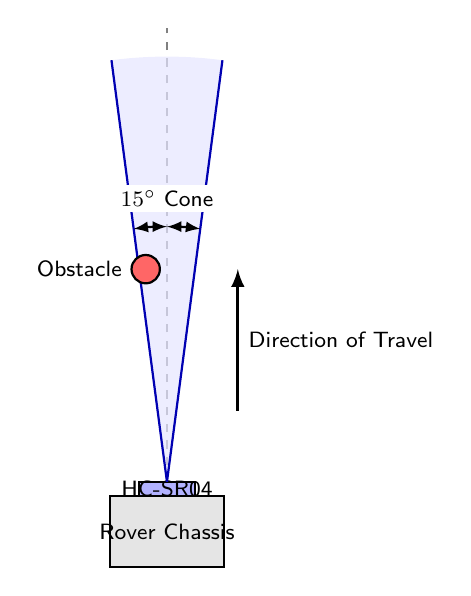
\begin{tikzpicture}[scale=0.18, >=latex, font=\sffamily\footnotesize]
        % Rover Chassis (Top View)
        \draw[fill=gray!20, thick] (-4, -5) rectangle (4, 0);
        \node at (0, -2.5) {Rover Chassis};

        % Ultrasonic Sensor (mounted at the front)
        \draw[fill=blue!30, thick] (-2, 0) rectangle (2, 1);
        \node at (0, 0.5) {HC-SR04};

        % Beam Cone (15 degrees total -> +/- 7.5 degrees from center)
        \begin{scope}[shift={(0,1)}]
            % Center line
            \draw[dashed, gray, thin] (0,0) -- (0,32);

            % Cone area
            \fill[blue!10, opacity=0.7] (0,0) -- (97.5:30) arc (97.5:82.5:30) -- cycle;
            % Cone edges
            \draw[blue!70!black, thick] (0,0) -- (97.5:30);
            \draw[blue!70!black, thick] (0,0) -- (82.5:30);

            % Angle Label
            \draw[<->, thick] (0, 18) arc (90:97.5:18);
            \draw[<->, thick] (0, 18) arc (90:82.5:18);
            \node[fill=white, inner sep=2pt] at (0, 20) {$15^\circ$ Cone};

            % Example Obstacle
            \draw[fill=red!60, thick] (-1.5, 15) circle (1);
            \node[left] at (-2.5, 15) {Obstacle};
            
            % Direction Arrow
            \draw[->, thick, very thick] (5, 5) -- (5, 15) node[midway, right] {Direction of Travel};
        \end{scope}
    \end{tikzpicture}
    \caption{Top-down view of the ultrasonic sensor's beam pattern. The narrow $15^\circ$ detection cone is shown relative to the rover chassis, detecting obstacles directly ahead.}
    \label{fig:ultrasonic-beam}
\end{figure}

\subsection{Level Shifting}

The HC-SR04 operates at 5V logic levels while the ESP32-S3 GPIO pins are 3.3V. The echo pin outputs 5V, which could damage the ESP32 input. A simple resistor voltage divider scales the echo signal down to 3.3V safe levels.

\begin{lstlisting}[caption={Voltage divider calculation}]
R1 = 1kOhm, R2 = 2kOhm
V_out = V_in * R2 / (R1 + R2)
V_out = 5V * 2k / 3k = 3.33V
\end{lstlisting}

% FIGURE PLACEHOLDER
\begin{figure}[H]
    \centering
    \includegraphics[width=0.6\textwidth]{figures/hardware/level_shifter_circuit.png}
    \caption{Resistor voltage divider for level shifting the 5V echo signal to 3.3V.}
    \label{fig:level-shifter}
\end{figure}

% --------------------------------------------------------
\section{Wiring and Interconnections}
\label{sec:wiring}

This section documents all electrical connections between components. Dupont jumper wires are used throughout for easy modification during development.

\subsection{Complete Wiring Diagram}

% FIGURE PLACEHOLDER
\begin{figure}[H]
    \centering
    \includegraphics[width=\textwidth]{figures/hardware/complete_wiring_diagram.jpg}
    \caption{Complete wiring diagram showing all connections between the ESP32-S3, L298N, motors, sensors, and power supply.}
    \label{fig:complete-wiring}
\end{figure}

\subsection{Wire Color Convention}

\begin{table}[h!]
    \centering
    \caption{Wire color coding standard}
    \label{tab:wire-colors}
    \begin{tabular}{ll}
        \toprule
        \textbf{Color} & \textbf{Purpose} \\
        \midrule
        Red    & Positive power (12V, 5V, 3.3V) \\
        Black  & Ground \\
        Yellow & Signal (GPIO outputs) \\
        Orange & Signal (GPIO inputs) \\
        Green  & I2C SDA \\
        Blue   & I2C SCL \\
        \bottomrule
    \end{tabular}
\end{table}

% FIGURE PLACEHOLDER
\begin{figure}[H]
    \centering
    \includegraphics[width=\textwidth]{figures/hardware/wiring_photo.jpg}
    \caption{Actual wiring on the prototype showing careful routing and color coding.}
    \label{fig:wiring-photo}
\end{figure}

% --------------------------------------------------------
\section{Assembly Process}
\label{sec:assembly}

The complete assembly follows a specific order to ensure proper fit and cable routing.

\subsection{Assembly Steps}

\begin{enumerate}
    \item Mount motors to chassis brackets using M3 screws
    \item Attach drive sprockets to motor shafts
    \item Install tracks with proper tension
    \item Mount battery holder to rear platform
    \item Attach L298N driver with standoffs
    \item Mount ESP32-S3 board adjacent to L298N
    \item Install ultrasonic sensor at front
    \item Mount camera module on adjustable bracket
    \item Complete all wiring connections
    \item Verify connections with multimeter before power on
\end{enumerate}

% FIGURE PLACEHOLDER
\begin{figure}[H]
    \centering
    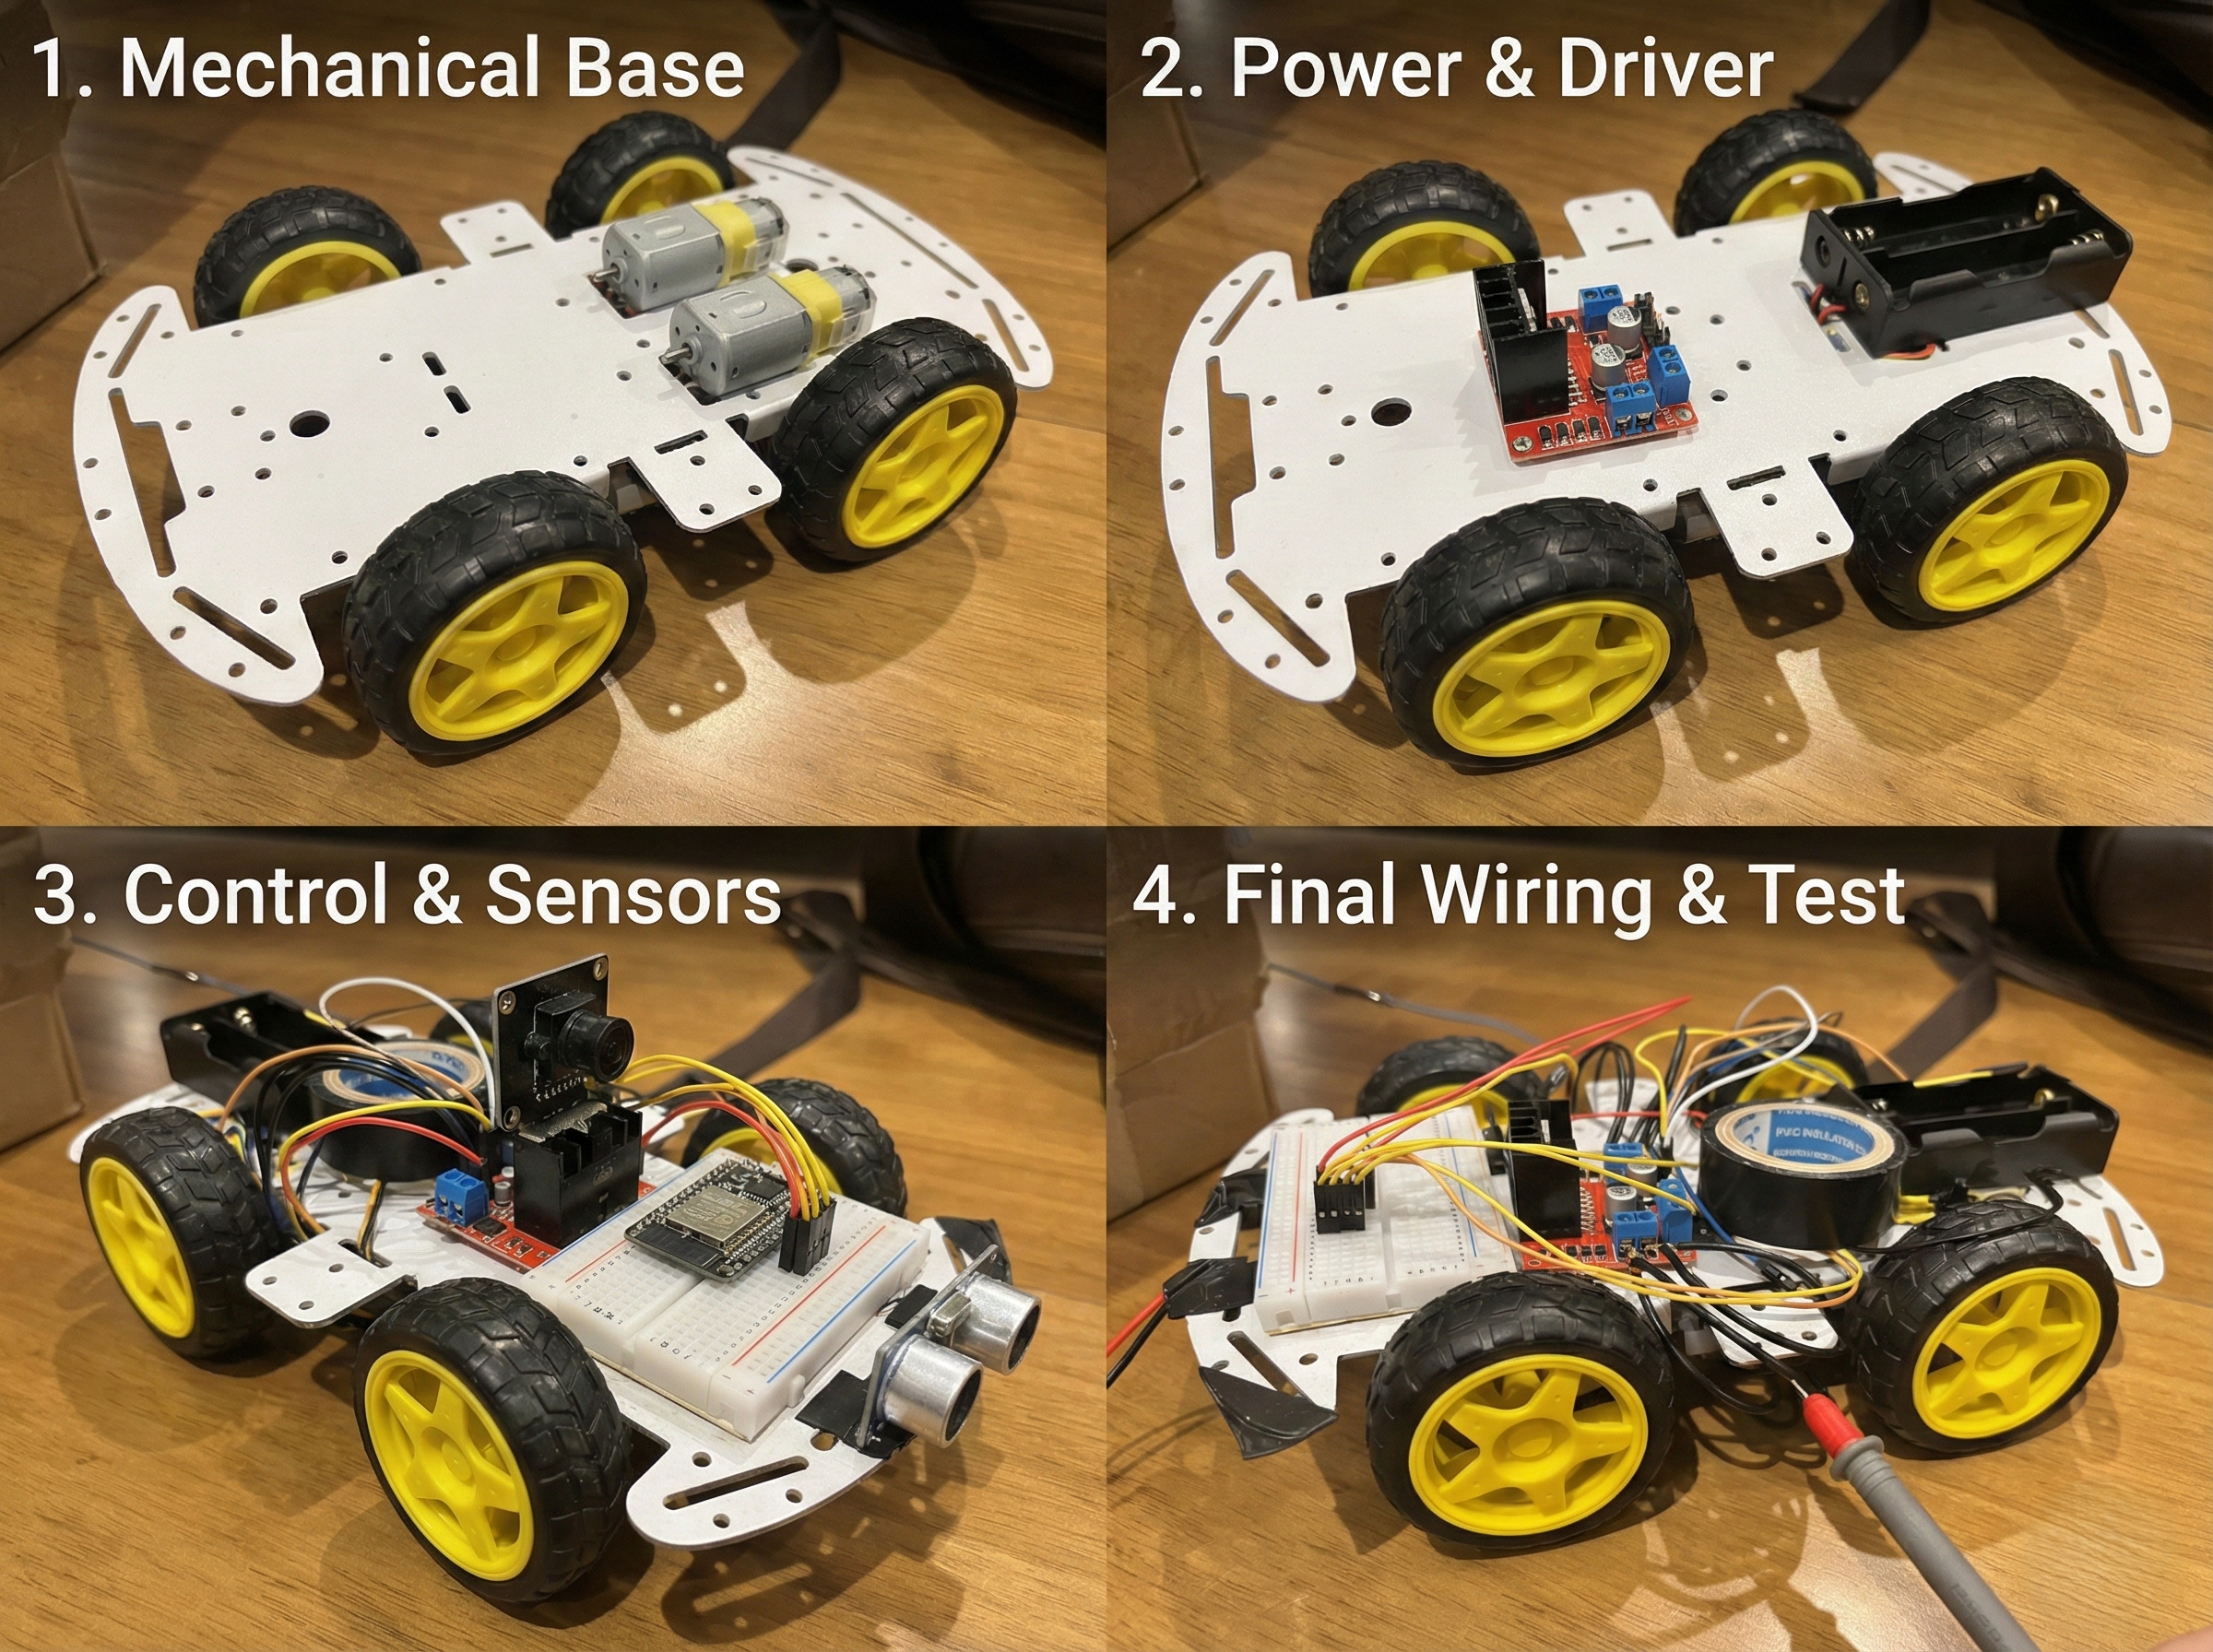
\includegraphics[width=\textwidth]{figures/hardware/assembly_sequence.png}
    \caption{Assembly sequence showing the progressive addition of components to the chassis.}
    \label{fig:assembly-sequence}
\end{figure}

\subsection{Testing Procedure}

After assembly, each subsystem is tested individually before full integration testing.

\begin{table}[h!]
    \centering
    \caption{Post-assembly test checklist}
    \label{tab:test-checklist}
    \begin{tabular}{lp{8cm}}
        \toprule
        \textbf{Subsystem} & \textbf{Test Procedure} \\
        \midrule
        Power     & Verify 5V and 3.3V rails with multimeter \\
        Motors    & Check rotation direction for each motor separately \\
        Camera    & Verify video feed appears in browser \\
        Ultrasonic & Move hand toward sensor, verify distance changes \\
        WiFi      & Confirm connection to access point \\
        ESP-NOW   & Verify command reception from gateway \\
        \bottomrule
    \end{tabular}
\end{table}

% FIGURE PLACEHOLDER
\begin{figure}[H]
    \centering
    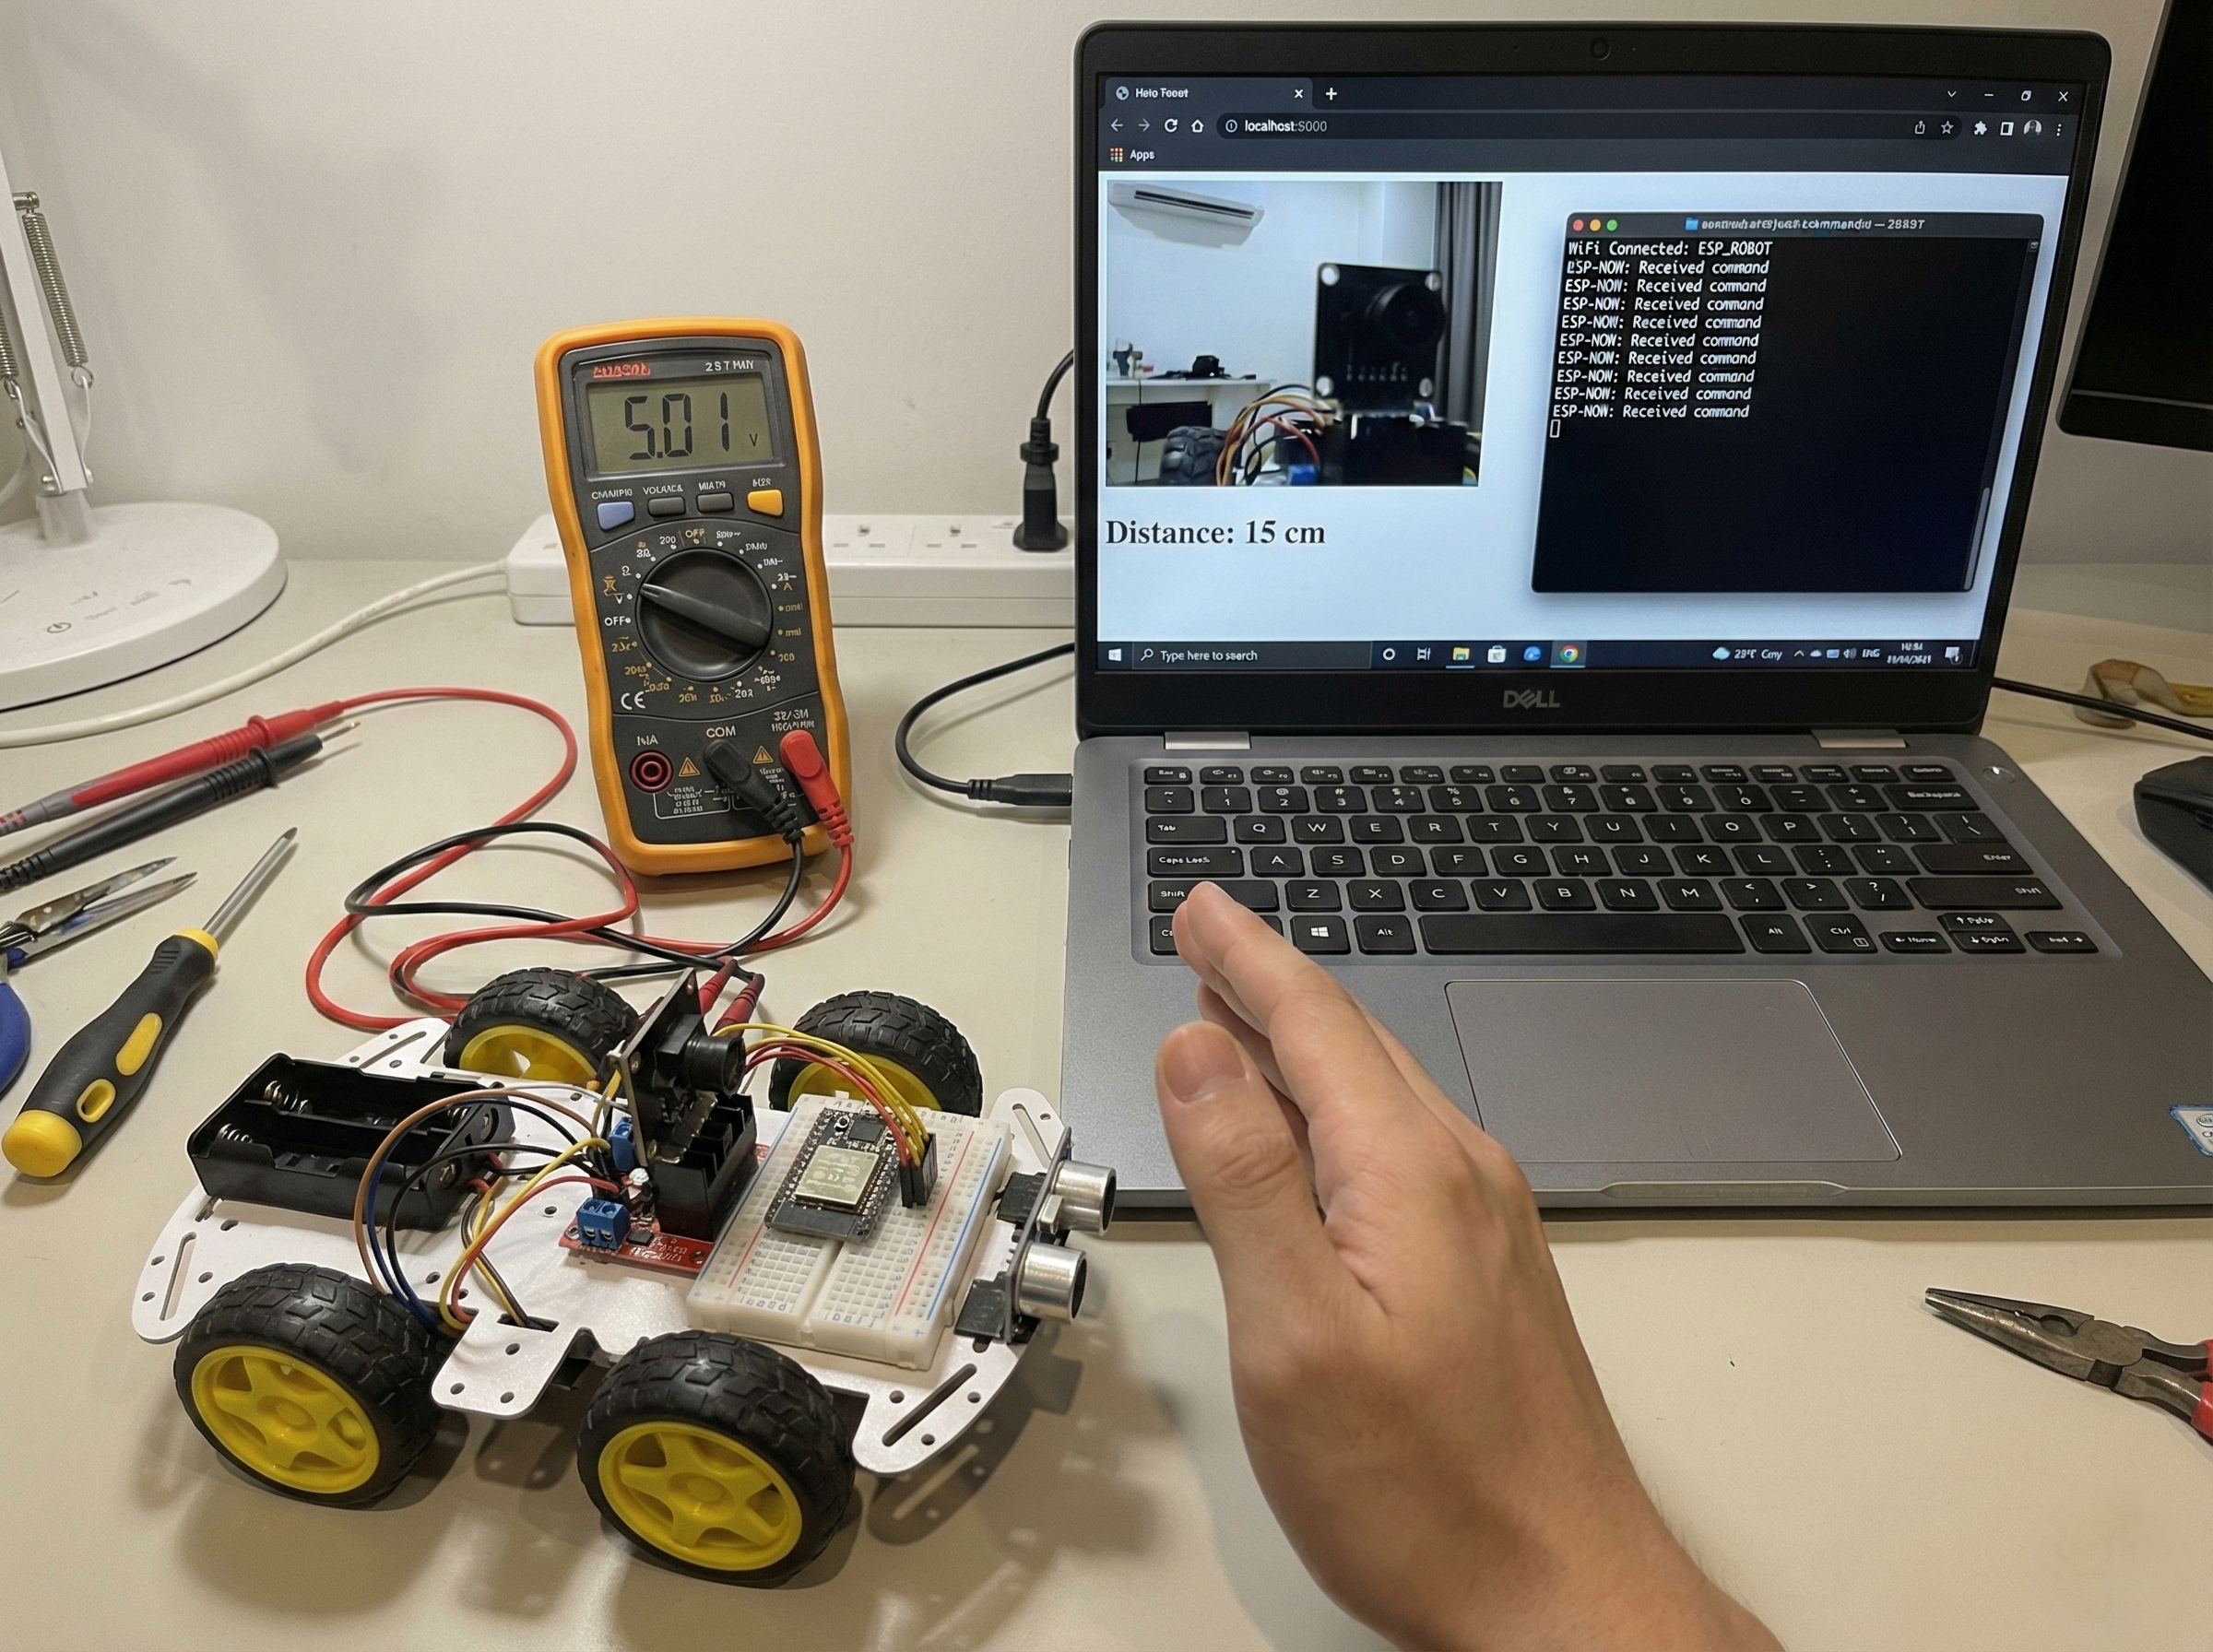
\includegraphics[width=\textwidth]{figures/hardware/testing_setup.png}
    \caption{Testing setup for post-assembly verification of subsystems.}
    \label{fig:testing-setup}
\end{figure}


% Chapter 4: Firmware Implementation
% chapters/04_firmware_implementation.tex - Chapter 4: Firmware Implementation
% =============================================================================

\chapter{Embedded Firmware Design}
\label{chap:firmware-implementation}

The firmware running on the ESP32-S3 forms the foundation of the Rescue Rover system. This chapter documents the design decisions, implementation details, and technical challenges encountered while developing the embedded software layer. The firmware handles camera streaming, motor control, wireless communication, and safety mechanisms, all running concurrently on the dual-core processor.

% --------------------------------------------------------
\section{Firmware Architecture Overview}
\label{sec:firmware-overview}

The ESP32-S3 firmware follows a modular architecture where each hardware subsystem is encapsulated in its own compilation unit. This separation allows independent development and testing of each component before integration. The project contains five primary modules, each with a specific responsibility in the system.

% FIGURE PLACEHOLDER
\begin{figure}[h!]
    \centering
    % \includegraphics[width=0.9\textwidth]{figures/software/firmware_architecture.png}
    \fbox{\parbox{0.9\textwidth}{\centering\vspace{3cm}FIGURE: Firmware Module Architecture Diagram\\Shows relationship between RescueRobot.ino, CameraModule, MotorDriver, ConnectionModule\vspace{3cm}}}
    \caption{Firmware module architecture showing the main sketch and its dependencies. The main loop coordinates all subsystems while individual modules manage their respective hardware interfaces.}
    \label{fig:firmware-architecture}
\end{figure}

\subsection{Module Responsibilities}

The \texttt{RescueRobot.ino} file serves as the main entry point. It initializes all hardware subsystems in a specific order and runs the main control loop at approximately 60Hz. The loop coordinates sensor readings, command processing, safety checks, and telemetry transmission. Total line count for this file is 265 lines.

The \texttt{CameraModule} handles all camera operations. This includes initialization of the OV2640 sensor, configuration of frame buffers in PSRAM, and streaming via either HTTP or UDP protocols. The module provides two streaming modes because we discovered during testing that HTTP introduces 80ms additional latency compared to UDP on the same network. Total implementation spans 222 lines across the header and source files.

The \texttt{MotorDriver} module controls the L298N H-bridge through GPIO pins. Movement primitives include forward, backward, left turn, right turn, and emergency stop. The implementation uses simple digital writes rather than PWM because the current prototype focuses on directional control rather than speed modulation. This module is intentionally minimal at 56 lines.

The \texttt{ConnectionModule} manages ESP-NOW bidirectional communication with the gateway. It receives joystick commands, stores them for processing by the main loop, and transmits telemetry at 2Hz. The critical design decision here is that the receive callback does not directly actuate motors. Instead it stores the command and lets the main loop apply safety checks first. This prevents race conditions between sensor readings and motor commands.

% FIGURE PLACEHOLDER
\begin{figure}[h!]
    \centering
    % \includegraphics[width=0.85\textwidth]{figures/software/module_dependencies.png}
    \fbox{\parbox{0.85\textwidth}{\centering\vspace{2.5cm}FIGURE: Module Dependency Graph\\Shows include relationships between all firmware files\vspace{2.5cm}}}
    \caption{Compilation dependencies between firmware modules. The main sketch includes all headers while modules only include what they need.}
    \label{fig:module-dependencies}
\end{figure}

\subsection{Memory Layout}

The ESP32-S3 provides multiple memory regions with different characteristics. Understanding these regions is essential for camera buffer allocation and overall system stability.

\begin{table}[h!]
    \centering
    \caption{ESP32-S3 memory regions and their usage in the firmware}
    \label{tab:memory-regions}
    \begin{tabular}{llp{6cm}}
        \toprule
        \textbf{Region} & \textbf{Size} & \textbf{Usage in Firmware} \\
        \midrule
        Internal SRAM    & 512 KB & Stack, heap, global variables, WiFi buffers \\
        PSRAM (External) & 8 MB   & Camera frame buffers (2 x 320x240), JPEG output buffer \\
        Flash            & 16 MB  & Program code, string constants, WiFi credentials \\
        \bottomrule
    \end{tabular}
\end{table}

Camera frame buffers consume the majority of PSRAM. Each QVGA frame requires 320 x 240 x 2 = 153.6 KB in YUV format. We allocate two buffers for double buffering, allowing one to be transmitted while the other captures the next frame. The JPEG compressed output typically ranges from 5 KB to 15 KB depending on scene complexity.

% FIGURE PLACEHOLDER
\begin{figure}[h!]
    \centering
    % \includegraphics[width=0.7\textwidth]{figures/hardware/esp32s3_memory_map.png}
    \fbox{\parbox{0.7\textwidth}{\centering\vspace{2.5cm}FIGURE: ESP32-S3 Memory Map\\Visual representation of SRAM, PSRAM, and Flash allocation\vspace{2.5cm}}}
    \caption{Memory allocation for the Rescue Rover firmware showing how camera buffers dominate PSRAM usage.}
    \label{fig:memory-map}
\end{figure}

% --------------------------------------------------------
\section{Camera Module Implementation}
\label{sec:camera-module-impl}

The camera module presented the most significant technical challenges during development. The OV2640 sensor requires precise timing, correct voltage levels, and specific initialization sequences. Several iterations were needed before achieving stable operation.

\subsection{Hardware Configuration}

The OV2640 connects to the ESP32-S3 through a DVP (Digital Video Port) interface. This parallel interface uses 8 data lines (D0-D7), synchronization signals (VSYNC, HREF, PCLK), and an I2C bus for register configuration.

% FIGURE PLACEHOLDER
\begin{figure}[h!]
    \centering
    % \includegraphics[width=\textwidth]{figures/hardware/camera_wiring_diagram.png}
    \fbox{\parbox{\textwidth}{\centering\vspace{4cm}FIGURE: OV2640 Camera Wiring Diagram\\Complete wiring between camera module ribbon cable and ESP32-S3 GPIO pins\vspace{4cm}}}
    \caption{Physical wiring between the OV2640 camera module and ESP32-S3 development board. The ribbon cable connects to a breakout board which then connects to individual GPIO pins.}
    \label{fig:camera-wiring}
\end{figure}

The pin mapping was derived from the Freenove ESP32-S3 WROOM CAM board schematic. However, our custom wiring required adjustments to avoid conflicts with motor control pins. The final configuration uses GPIO 10 for XCLK, GPIO 40 and 39 for I2C, and GPIO 38 for VSYNC. Data pins span GPIO 11 through 18 and GPIO 48.

\begin{lstlisting}[language=C++, caption={Camera pin configuration from CameraPins.h}]
// ESP32-S3 Camera Pin Mapping (Freenove Compatible)
#define PWDN_GPIO_NUM     -1   // Not connected
#define RESET_GPIO_NUM    -1   // Using software reset
#define XCLK_GPIO_NUM     10   // Master clock output
#define SIOD_GPIO_NUM     40   // I2C SDA
#define SIOC_GPIO_NUM     39   // I2C SCL
#define Y9_GPIO_NUM       48   // Data bit 7
#define Y8_GPIO_NUM       11   // Data bit 6
#define Y7_GPIO_NUM       12   // Data bit 5
#define Y6_GPIO_NUM       14   // Data bit 4
#define Y5_GPIO_NUM       16   // Data bit 3
#define Y4_GPIO_NUM       18   // Data bit 2
#define Y3_GPIO_NUM       17   // Data bit 1
#define Y2_GPIO_NUM       15   // Data bit 0
#define VSYNC_GPIO_NUM    38   // Vertical sync
#define HREF_GPIO_NUM     47   // Horizontal reference
#define PCLK_GPIO_NUM     13   // Pixel clock
\end{lstlisting}

\subsection{Initialization Sequence}

Camera initialization follows a strict sequence. Any deviation results in cryptic error codes or complete failure to capture frames. We reduced the XCLK frequency from 20MHz to 10MHz after encountering intermittent initialization failures. The lower clock speed sacrifices theoretical maximum framerate but dramatically improves reliability.

\begin{algorithm}[h!]
    \caption{Camera Initialization Sequence}
    \label{alg:camera-init-full}
    \begin{algorithmic}[1]
        \STATE Check for PSRAM availability
        \IF{PSRAM not found}
            \STATE Log warning: camera may fail without external memory
        \ENDIF
        \STATE Populate \texttt{camera\_config\_t} structure with pin numbers
        \STATE Set XCLK frequency to 10 MHz (conservative setting)
        \STATE Set frame size to QVGA (320 x 240 pixels)
        \STATE Set pixel format to JPEG with quality level 30
        \STATE Set frame buffer location to PSRAM
        \STATE Allocate 2 frame buffers for double buffering
        \STATE Set grab mode to CAMERA\_GRAB\_LATEST
        \STATE Call \func{esp\_camera\_init} with configuration
        \IF{initialization returns error}
            \STATE Log error code and halt
            \RETURN false
        \ENDIF
        \STATE Get sensor handle via \func{esp\_camera\_sensor\_get}
        \STATE Disable test pattern (colorbar) for real images
        \STATE Log success message with resolution
        \RETURN true
    \end{algorithmic}
\end{algorithm}

% FIGURE PLACEHOLDER
\begin{figure}[h!]
    \centering
    % \includegraphics[width=0.8\textwidth]{figures/software/camera_init_flowchart.png}
    \fbox{\parbox{0.8\textwidth}{\centering\vspace{3cm}FIGURE: Camera Initialization Flowchart\\Decision tree showing PSRAM check, config, init, and error handling paths\vspace{3cm}}}
    \caption{Flowchart for camera initialization showing fail-safe checks and configuration steps.}
    \label{fig:camera-init-flow}
\end{figure}

The JPEG quality parameter inversely correlates with file size. A quality value of 30 produces frames between 5KB and 12KB, suitable for UDP transmission within a single packet on local networks. Lower quality values (higher numbers in the ESP camera API) create smaller files but introduce visible compression artifacts.

\subsection{Streaming Modes}

The firmware supports two distinct streaming protocols. HTTP MJPEG provides browser compatibility and easy debugging. UDP streaming minimizes latency for the AI processing pipeline.

\subsubsection{HTTP MJPEG Streaming}

The HTTP mode creates a simple web server on port 80 with a single endpoint at \texttt{/stream}. When a client connects, the handler enters an infinite loop, capturing frames and sending them with multipart boundaries. This approach works with any web browser and requires no client side code.

\begin{lstlisting}[language=C++, caption={HTTP MJPEG stream handler implementation}]
static esp_err_t stream_handler(httpd_req_t *req) {
    camera_fb_t *fb = NULL;
    esp_err_t res = ESP_OK;
    char part_buf[64];
    
    // Set content type for MJPEG stream
    res = httpd_resp_set_type(req, 
        "multipart/x-mixed-replace;boundary=frame");
    if (res != ESP_OK) return res;
    
    while (true) {
        fb = esp_camera_fb_get();
        if (!fb) {
            Serial.println("Capture failed");
            res = ESP_FAIL;
        } else {
            // Build multipart header
            size_t hlen = snprintf(part_buf, 64,
                "\r\n--frame\r\n"
                "Content-Type: image/jpeg\r\n"
                "Content-Length: %u\r\n\r\n", fb->len);
            
            res = httpd_resp_send_chunk(req, part_buf, hlen);
            if (res == ESP_OK) {
                res = httpd_resp_send_chunk(req, 
                    (const char*)fb->buf, fb->len);
            }
            esp_camera_fb_return(fb);
        }
        if (res != ESP_OK) break;
    }
    return res;
}
\end{lstlisting}

% FIGURE PLACEHOLDER
\begin{figure}[h!]
    \centering
    % \includegraphics[width=0.8\textwidth]{figures/software/http_stream_sequence.png}
    \fbox{\parbox{0.8\textwidth}{\centering\vspace{3cm}FIGURE: HTTP MJPEG Sequence Diagram\\Shows request/response flow between browser and ESP32-S3\vspace{3cm}}}
    \caption{Sequence diagram for HTTP MJPEG streaming showing the continuous frame transmission loop.}
    \label{fig:http-sequence}
\end{figure}

\subsubsection{UDP Streaming}

UDP mode sends frames directly without the HTTP overhead. The target IP address and port are configured at compile time. Each frame is transmitted as a single UDP packet, which works reliably on local networks where MTU is 1500 bytes and frames are under 15KB.

\begin{lstlisting}[language=C++, caption={UDP frame transmission function}]
void streamFrameUDP() {
    // Check prerequisites
    if (!cameraReady || !udpMode || udpTargetIP == nullptr)
        return;
    
    camera_fb_t *fb = esp_camera_fb_get();
    if (!fb) {
        Serial.println("UDP capture failed");
        return;
    }
    
    // Send entire frame as single packet
    // Works on local WiFi where fragmentation is handled
    udp.beginPacket(udpTargetIP, udpTargetPort);
    udp.write(fb->buf, fb->len);
    udp.endPacket();
    
    esp_camera_fb_return(fb);
}
\end{lstlisting}

% FIGURE PLACEHOLDER
\begin{figure}[h!]
    \centering
    % \includegraphics[width=0.85\textwidth]{figures/charts/http_vs_udp_latency.png}
    \fbox{\parbox{0.85\textwidth}{\centering\vspace{3cm}FIGURE: HTTP vs UDP Latency Comparison\\Bar chart showing measured latency for both protocols\vspace{3cm}}}
    \caption{Measured latency comparison between HTTP MJPEG and UDP streaming modes. UDP consistently shows 80ms lower latency.}
    \label{fig:latency-comparison}
\end{figure}

\begin{table}[h!]
    \centering
    \caption{Comparison of streaming modes}
    \label{tab:streaming-comparison}
    \begin{tabular}{lcc}
        \toprule
        \textbf{Characteristic} & \textbf{HTTP MJPEG} & \textbf{UDP Direct} \\
        \midrule
        End to end latency      & 180-220 ms    & 100-140 ms \\
        Browser compatible      & Yes           & No (requires custom receiver) \\
        Packet loss handling    & TCP retransmit & None (frames dropped) \\
        Setup complexity        & Low           & Medium \\
        Network overhead        & Higher        & Lower \\
        Recommended use         & Debugging     & Production \\
        \bottomrule
    \end{tabular}
\end{table}

% --------------------------------------------------------
\section{Motor Control Implementation}
\label{sec:motor-impl}

The motor control subsystem translates high level movement commands into GPIO signals for the L298N driver. The current implementation uses binary on/off control rather than PWM speed modulation. This choice simplifies the code and proved sufficient for indoor testing where precise speed control is less important than reliable direction changes.

\subsection{Differential Drive Model}

The rover uses a differential drive configuration with two independently controlled motors. This arrangement allows the robot to turn by varying the relative speeds of the left and right wheels. Mathematically, the relationship between wheel velocities and robot motion is expressed as:

\begin{equation}
    v_{robot} = \frac{v_R + v_L}{2}
    \label{eq:linear-vel}
\end{equation}

\begin{equation}
    \omega_{robot} = \frac{v_R - v_L}{W}
    \label{eq:angular-vel}
\end{equation}

where $v_{robot}$ is the linear velocity of the robot center, $\omega_{robot}$ is the angular velocity, $v_R$ and $v_L$ are the right and left wheel velocities respectively, and $W$ is the wheelbase width.

% FIGURE PLACEHOLDER
\begin{figure}[h!]
    \centering
    % \includegraphics[width=0.6\textwidth]{figures/hardware/differential_drive_kinematics.png}
    \fbox{\parbox{0.6\textwidth}{\centering\vspace{3cm}FIGURE: Differential Drive Kinematics\\Diagram showing wheel velocities, turning radius, and angular velocity\vspace{3cm}}}
    \caption{Differential drive kinematic model showing how independent wheel speeds create linear and angular motion.}
    \label{fig:diff-drive}
\end{figure}

\subsection{L298N Driver Interface}

The L298N accepts four digital inputs (IN1 through IN4) that control two H-bridge circuits. Each motor connects to one H-bridge. The truth table for motor direction is straightforward: setting one input HIGH and the other LOW drives the motor in one direction. Reversing which input is HIGH reverses the rotation.

\begin{lstlisting}[language=C++, caption={Motor driver initialization and movement functions}]
#include "MotorDriver.h"
#include "PinConfig.h"

void initMotors() {
    pinMode(PIN_LEFT_FWD, OUTPUT);
    pinMode(PIN_LEFT_BWD, OUTPUT);
    pinMode(PIN_RIGHT_FWD, OUTPUT);
    pinMode(PIN_RIGHT_BWD, OUTPUT);
    
    stopMoving();  // Ensure motors are off at startup
    Serial.println("Motor Driver Ready (GPIO: 4,5,6,7)");
}

void goForward() {
    digitalWrite(PIN_LEFT_FWD, HIGH);
    digitalWrite(PIN_LEFT_BWD, LOW);
    digitalWrite(PIN_RIGHT_FWD, HIGH);
    digitalWrite(PIN_RIGHT_BWD, LOW);
}

void goBackward() {
    digitalWrite(PIN_LEFT_FWD, LOW);
    digitalWrite(PIN_LEFT_BWD, HIGH);
    digitalWrite(PIN_RIGHT_FWD, LOW);
    digitalWrite(PIN_RIGHT_BWD, HIGH);
}

void stopMoving() {
    digitalWrite(PIN_LEFT_FWD, LOW);
    digitalWrite(PIN_LEFT_BWD, LOW);
    digitalWrite(PIN_RIGHT_FWD, LOW);
    digitalWrite(PIN_RIGHT_BWD, LOW);
}
\end{lstlisting}

% FIGURE PLACEHOLDER
\begin{figure}[h!]
    \centering
    % \includegraphics[width=0.9\textwidth]{figures/hardware/l298n_wiring.png}
    \fbox{\parbox{0.9\textwidth}{\centering\vspace{3.5cm}FIGURE: L298N Motor Driver Wiring\\Complete schematic showing ESP32-S3 GPIO connections, motor terminals, and power input\vspace{3.5cm}}}
    \caption{L298N motor driver wiring diagram showing all connections between ESP32-S3, the driver board, and both DC motors.}
    \label{fig:l298n-wiring}
\end{figure}

\subsection{Pin Assignment}

The motor pins were chosen to avoid conflicts with camera interface and JTAG debugging. GPIO 4, 5, 6, and 7 are safe choices that do not overlap with any other peripheral.

\begin{table}[h!]
    \centering
    \caption{Motor driver pin assignment}
    \label{tab:motor-pins}
    \begin{tabular}{llll}
        \toprule
        \textbf{Function} & \textbf{L298N Pin} & \textbf{ESP32 GPIO} & \textbf{Wire Color} \\
        \midrule
        Left Forward   & IN1 & GPIO 4 & Yellow \\
        Left Backward  & IN2 & GPIO 5 & Orange \\
        Right Forward  & IN3 & GPIO 6 & Green \\
        Right Backward & IN4 & GPIO 7 & Blue \\
        \bottomrule
    \end{tabular}
\end{table}

\subsection{Turning Mechanics}

Point turns are achieved by running motors in opposite directions. The left motor runs backward while the right motor runs forward for a left turn. This creates rotation around the robot's center point. Arc turns for smoother motion would require PWM speed control, which is planned for a future revision.

% FIGURE PLACEHOLDER
\begin{figure}[h!]
    \centering
    % \includegraphics[width=0.8\textwidth]{figures/hardware/turn_mechanics.png}
    \fbox{\parbox{0.8\textwidth}{\centering\vspace{3cm}FIGURE: Turning Mechanics Diagram\\Shows point turn vs arc turn wheel direction arrows\vspace{3cm}}}
    \caption{Comparison of point turn (current implementation) versus arc turn (future enhancement). Point turns rotate in place while arc turns follow a curved path.}
    \label{fig:turn-mechanics}
\end{figure}

% --------------------------------------------------------
\section{ESP-NOW Communication Module}
\label{sec:espnow-impl}

The ConnectionModule handles all wireless communication between the rover and the gateway device. ESP-NOW was selected over TCP/IP for control commands because it offers significantly lower latency. The protocol operates at the MAC layer, bypassing much of the WiFi stack overhead.

\subsection{Protocol Overview}

ESP-NOW allows direct device to device communication using MAC addresses. Packets are limited to 250 bytes, but this is more than sufficient for joystick commands (8 bytes) and telemetry (8 bytes). The protocol does not guarantee delivery, but at close range with clear line of sight, packet loss is negligible.

% FIGURE PLACEHOLDER
\begin{figure}[h!]
    \centering
    % \includegraphics[width=\textwidth]{figures/software/espnow_protocol_stack.png}
    \fbox{\parbox{\textwidth}{\centering\vspace{3cm}FIGURE: ESP-NOW Protocol Stack\\Shows position in networking layers compared to standard WiFi TCP/IP\vspace{3cm}}}
    \caption{ESP-NOW protocol positioning in the network stack. It operates below IP, directly on top of the 802.11 MAC layer.}
    \label{fig:espnow-stack}
\end{figure}

\subsection{Packet Structures}

Two packet types define the communication protocol. The command structure carries joystick X and Y values from the gateway to the rover. The feedback structure carries voltage and distance readings from the rover back to the gateway.

\begin{lstlisting}[language=C++, caption={ESP-NOW packet structure definitions}]
// Command packet: Gateway -> Rover
typedef struct __attribute__((packed)) command_struct {
    int x;  // Joystick X (0-4095, center=2048)
    int y;  // Joystick Y (0-4095, center=2048)
} command_struct;

// Feedback packet: Rover -> Gateway
typedef struct __attribute__((packed)) feedback_struct {
    float voltage;   // Battery voltage in volts
    int distance;    // Ultrasonic distance in cm
} feedback_struct;
\end{lstlisting}

The \texttt{\_\_attribute\_\_((packed))} directive ensures no padding bytes are inserted between structure members. This guarantees the structure has the exact same memory layout on both ESP32 devices.

% FIGURE PLACEHOLDER
\begin{figure}[h!]
    \centering
    % \includegraphics[width=0.7\textwidth]{figures/software/packet_format.png}
    \fbox{\parbox{0.7\textwidth}{\centering\vspace{2.5cm}FIGURE: Packet Format Diagram\\Shows byte layout of command and feedback structures\vspace{2.5cm}}}
    \caption{Binary layout of ESP-NOW packet structures showing byte offsets for each field.}
    \label{fig:packet-format}
\end{figure}

\subsection{Receive Callback Design}

The receive callback executes in an interrupt context when a packet arrives. Long operations in this callback would block the WiFi stack and cause instability. Our initial implementation called motor control functions directly from the callback, which created race conditions with the ultrasonic sensor readings in the main loop.

\begin{designbox}[Critical Design Decision: Deferred Motor Actuation]
The receive callback stores commands but does not actuate motors. Motor actuation happens in the main loop after safety checks. This prevents race conditions where an obstacle appears between receiving a "forward" command and executing it. The main loop always has the latest sensor data when deciding whether to execute a command.
\end{designbox}

\begin{lstlisting}[language=C++, caption={ESP-NOW receive callback with deferred actuation}]
// State variables
static command_struct recvCommand = {2048, 2048};  // Center = stop
static unsigned long lastPacketTime = 0;

// Callback: ONLY stores command, does NOT control motors
static void onDataRecv(const esp_now_recv_info_t *info,
                       const uint8_t *data, int len) {
    if (len != sizeof(command_struct)) {
        Serial.printf("Wrong packet size: %d\n", len);
        return;
    }
    
    // Store command for main loop to process
    memcpy(&recvCommand, data, sizeof(recvCommand));
    
    // Update heartbeat timestamp
    lastPacketTime = millis();
    
    Serial.printf("RX: X=%d Y=%d\n", recvCommand.x, recvCommand.y);
}
\end{lstlisting}

% FIGURE PLACEHOLDER
\begin{figure}[h!]
    \centering
    % \includegraphics[width=\textwidth]{figures/software/callback_vs_loop_diagram.png}
    \fbox{\parbox{\textwidth}{\centering\vspace{3cm}FIGURE: Callback vs Main Loop Processing\\Sequence showing how commands flow from ESP-NOW to motor actuation\vspace{3cm}}}
    \caption{Data flow from ESP-NOW callback to motor actuation through the main loop safety checks.}
    \label{fig:callback-flow}
\end{figure}

\subsection{Telemetry Transmission}

Telemetry is sent at 2Hz (every 500ms) to avoid flooding the wireless channel. The feedback packet contains battery voltage and ultrasonic distance. The gateway forwards this data to the dashboard over USB serial.

\begin{lstlisting}[language=C++, caption={Telemetry transmission with rate limiting}]
static unsigned long lastTelemetryTime = 0;
static const unsigned long TELEMETRY_INTERVAL = 500;  // 2Hz

void handleConnection(float voltage, int distance) {
    unsigned long now = millis();
    
    // Rate limit to 2Hz
    if (now - lastTelemetryTime >= TELEMETRY_INTERVAL) {
        lastTelemetryTime = now;
        
        sendFeedback.voltage = voltage;
        sendFeedback.distance = distance;
        
        esp_err_t result = esp_now_send(
            gatewayMAC, 
            (uint8_t*)&sendFeedback, 
            sizeof(sendFeedback)
        );
        
        if (result != ESP_OK) {
            Serial.println("Telemetry send failed");
        }
    }
}
\end{lstlisting}

% --------------------------------------------------------
\section{Safety Mechanisms}
\label{sec:safety-mechanisms}

The firmware implements multiple layers of safety to prevent the rover from colliding with obstacles or running away if communication is lost. These mechanisms operate at the firmware level where response time is guaranteed.

\subsection{Heartbeat Failsafe}

If no command packet arrives within 500ms, the rover assumes communication has been lost and stops all motors. This prevents the rover from continuing to execute a stale "forward" command indefinitely. The timeout value was chosen based on the expected packet rate of 20Hz from the joystick.

\begin{lstlisting}[language=C++, caption={Heartbeat check in main control loop}]
const unsigned long SIGNAL_TIMEOUT = 500;  // 500ms

void handleControlLoop() {
    // Check connection heartbeat
    if (!isConnectionAlive(SIGNAL_TIMEOUT)) {
        static bool signalLostPrinted = false;
        if (!signalLostPrinted) {
            Serial.println("SIGNAL LOST - EMERGENCY STOP!");
            signalLostPrinted = true;
        }
        stopMoving();
        return;  // Skip all control logic
    }
    
    // ... rest of control logic
}

bool isConnectionAlive(unsigned long timeoutMs) {
    if (lastPacketTime == 0) return true;  // Allow startup
    return (millis() - lastPacketTime) < timeoutMs;
}
\end{lstlisting}

% FIGURE PLACEHOLDER
\begin{figure}[h!]
    \centering
    % \includegraphics[width=0.85\textwidth]{figures/software/heartbeat_state_machine.png}
    \fbox{\parbox{0.85\textwidth}{\centering\vspace{3cm}FIGURE: Heartbeat State Machine\\Shows CONNECTED, WARNING, and STOPPED states with transitions\vspace{3cm}}}
    \caption{State machine for heartbeat monitoring showing transitions between connected and stopped states.}
    \label{fig:heartbeat-fsm}
\end{figure}

\subsection{Ultrasonic Obstacle Detection}

The ultrasonic sensor provides distance measurements to the nearest obstacle in the forward direction. The firmware uses this to override forward commands when an obstacle is too close. The implementation uses a state machine rather than the blocking \texttt{pulseIn()} function to avoid freezing the main loop.

\begin{lstlisting}[language=C++, caption={Non-blocking ultrasonic state machine}]
enum UltrasonicState {
    US_IDLE,
    US_TRIGGER_HIGH,
    US_WAIT_ECHO_START,
    US_WAIT_ECHO_END
};

static UltrasonicState usState = US_IDLE;
static unsigned long usTriggerTime = 0;
static unsigned long usEchoStart = 0;

bool updateUltrasonicDistance() {
    unsigned long now = micros();
    
    switch (usState) {
    case US_IDLE:
        digitalWrite(TRIG_PIN, HIGH);
        usTriggerTime = now;
        usState = US_TRIGGER_HIGH;
        break;
        
    case US_TRIGGER_HIGH:
        if (now - usTriggerTime >= 10) {  // 10us trigger pulse
            digitalWrite(TRIG_PIN, LOW);
            usState = US_WAIT_ECHO_START;
        }
        break;
        
    case US_WAIT_ECHO_START:
        if (digitalRead(ECHO_PIN) == HIGH) {
            usEchoStart = now;
            usState = US_WAIT_ECHO_END;
        } else if (now - usTriggerTime > 30000) {  // 30ms timeout
            currentDistance = 999;  // No object detected
            usState = US_IDLE;
            return true;
        }
        break;
        
    case US_WAIT_ECHO_END:
        if (digitalRead(ECHO_PIN) == LOW) {
            unsigned long duration = now - usEchoStart;
            currentDistance = (duration * 0.034) / 2;  // Speed of sound
            usState = US_IDLE;
            return true;
        } else if (now - usEchoStart > 30000) {  // Timeout
            currentDistance = 999;
            usState = US_IDLE;
            return true;
        }
        break;
    }
    return false;
}
\end{lstlisting}

% FIGURE PLACEHOLDER
\begin{figure}[h!]
    \centering
    % \includegraphics[width=\textwidth]{figures/software/ultrasonic_state_machine.png}
    \fbox{\parbox{\textwidth}{\centering\vspace{3.5cm}FIGURE: Ultrasonic State Machine\\Shows all states with timing conditions for transitions\vspace{3.5cm}}}
    \caption{State machine diagram for non-blocking ultrasonic distance measurement.}
    \label{fig:ultrasonic-fsm}
\end{figure}

\subsection{Unified Control Loop}

The main control loop integrates all sensor inputs and safety checks before executing motor commands. This unified approach ensures that no command is executed without considering the current safety state.

\begin{lstlisting}[language=C++, caption={Unified control loop with safety integration}]
const int EMERGENCY_STOP_DISTANCE = 25;  // cm

void handleControlLoop() {
    // 0. Check heartbeat (covered above)
    
    // 1. Update distance sensor (non-blocking)
    updateUltrasonicDistance();
    
    // 2. Get latest joystick command
    command_struct cmd = getLastCommand();
    
    // 3. Is rover trying to move forward?
    bool tryingToMoveForward = (cmd.y > 2500);
    
    // 4. Safety decision matrix
    if (currentDistance < EMERGENCY_STOP_DISTANCE 
        && tryingToMoveForward) {
        // Block forward movement
        if (!emergencyStopActive) {
            Serial.printf("OBSTACLE at %d cm - BLOCKING!\n", 
                currentDistance);
            stopMoving();
            emergencyStopActive = true;
        }
        
        // But allow backward/turning to escape
        if (cmd.y < 1500 || cmd.x < 1000 || cmd.x > 3000) {
            Serial.println("Escape maneuver allowed");
            executeMotorCommand(cmd.x, cmd.y);
            emergencyStopActive = false;
        }
    } else {
        // Safe to execute command
        emergencyStopActive = false;
        executeMotorCommand(cmd.x, cmd.y);
    }
}
\end{lstlisting}

% FIGURE PLACEHOLDER
\begin{figure}[h!]
    \centering
    % \includegraphics[width=\textwidth]{figures/software/control_loop_flowchart.png}
    \fbox{\parbox{\textwidth}{\centering\vspace{4cm}FIGURE: Unified Control Loop Flowchart\\Complete decision tree showing heartbeat, distance, and command processing\vspace{4cm}}}
    \caption{Flowchart of the unified control loop showing all safety checks and their precedence.}
    \label{fig:control-loop-flow}
\end{figure}

\begin{table}[h!]
    \centering
    \caption{Safety mechanism summary}
    \label{tab:safety-summary}
    \begin{tabular}{llp{5cm}}
        \toprule
        \textbf{Mechanism} & \textbf{Trigger} & \textbf{Action} \\
        \midrule
        Heartbeat failsafe & No packets for 500ms & Stop all motors \\
        Obstacle blocking  & Distance < 25cm + forward command & Block forward, allow escape \\
        Slow zone          & Distance 25-50cm & (Future: reduce speed) \\
        Watchdog timer     & Firmware hang & Hardware reset \\
        \bottomrule
    \end{tabular}
\end{table}

% --------------------------------------------------------
\section{Main Loop Structure}
\label{sec:main-loop}

The main loop in \texttt{RescueRobot.ino} coordinates all subsystems at approximately 60Hz. Each iteration performs control processing, video streaming (if UDP mode), and telemetry transmission.

\begin{lstlisting}[language=C++, caption={Main application loop}]
void loop() {
    // 1. Unified Control Loop
    //    (sensor reading + safety checks + motor actuation)
    handleControlLoop();
    
    // 2. Stream video frame (UDP mode only)
    if (USE_UDP_STREAM) {
        streamFrameUDP();
    }
    
    // 3. Transmit telemetry (rate limited to 2Hz internally)
    handleConnection(BATTERY_VOLTAGE, currentDistance);
    
    // 4. Small delay to prevent watchdog triggers
    delay(5);
}
\end{lstlisting}

The 5ms delay at the end of each loop iteration ensures the watchdog timer is not triggered by tight loops. This delay also provides time for the WiFi stack to process incoming packets between iterations.

% FIGURE PLACEHOLDER
\begin{figure}[h!]
    \centering
    % \includegraphics[width=0.7\textwidth]{figures/software/loop_timing_diagram.png}
    \fbox{\parbox{0.7\textwidth}{\centering\vspace{3cm}FIGURE: Main Loop Timing Diagram\\Shows time allocation for each subsystem per iteration\vspace{3cm}}}
    \caption{Timing breakdown of a single main loop iteration showing relative time spent in each subsystem.}
    \label{fig:loop-timing}
\end{figure}

% --------------------------------------------------------
\section{Compilation and Deployment}
\label{sec:compilation}

The firmware is developed using the Arduino framework with ESP32 board support. Compilation requires specific board settings to enable PSRAM and select the correct partition scheme.

\begin{table}[h!]
    \centering
    \caption{Arduino IDE board configuration}
    \label{tab:arduino-config}
    \begin{tabular}{ll}
        \toprule
        \textbf{Setting} & \textbf{Value} \\
        \midrule
        Board           & ESP32S3 Dev Module \\
        PSRAM           & OPI PSRAM \\
        Flash Mode      & QIO 80MHz \\
        Flash Size      & 16MB \\
        Partition Scheme & Huge APP (3MB No OTA / 1MB SPIFFS) \\
        Upload Speed    & 921600 \\
        \bottomrule
    \end{tabular}
\end{table}

The "Huge APP" partition scheme allocates maximum space for application code, which is necessary given the size of the camera driver library. OTA (over the air) updates are disabled in exchange for the larger application partition.

% FIGURE PLACEHOLDER
\begin{figure}[h!]
    \centering
    % \includegraphics[width=0.8\textwidth]{figures/software/arduino_board_settings.png}
    \fbox{\parbox{0.8\textwidth}{\centering\vspace{3cm}FIGURE: Arduino IDE Board Settings Screenshot\\Shows Tools menu with all required settings highlighted\vspace{3cm}}}
    \caption{Arduino IDE Tools menu configuration for ESP32-S3 with PSRAM enabled.}
    \label{fig:arduino-settings}
\end{figure}


% Chapter 5: AI & Software Design
% chapters/05_ai_software_design.tex - Chapter 5: AI & Software Design
% =====================================================================

\chapter{AI \& Software Design}
\label{chap:ai-software-design}

This chapter documents the software architecture of the host application and its integration with cloud-based AI services. The design uses a "Hybrid Cloud" approach: real-time tactical processing runs locally on the host computer, while complex strategic reasoning is offloaded to a cloud server equipped with high-performance GPUs.

% --------------------------------------------------------
\section{Host Application Architecture}
\label{sec:host-architecture}

The RoverInterface application acts as the central coordinator. It manages three critical loops running at different frequencies:
1.  \textbf{The Control Loop (100Hz)}: Reads joystick inputs and sends serial commands.
2.  \textbf{The Tactical Loop (30Hz)}: Captures video and runs local object detection (YOLO).
3.  \textbf{The Strategic Loop (0.5Hz)}: Asynchronously sends frames to the cloud for detailed analysis.

% FIGURE PLACEHOLDER
\begin{figure}[h!]
    \centering
    \includegraphics[width=\textwidth]{figures/software/host_architecture_hybrid.png}
    \caption{High level architecture showing the split between local processing and cloud delegation.}
    \label{fig:host-architecture}
\end{figure}

\subsection{Tech Stack Changes for Hybrid Cloud}

To support this architecture, the software stack includes networking components to reliably bridge the local application with the cloud instance.

\begin{table}[h!]
    \centering
    \caption{Software components and roles}
    \label{tab:python-deps}
    \begin{tabular}{llp{6cm}}
        \toprule
        \textbf{Component} & \textbf{Type} & \textbf{Purpose} \\
        \midrule
        NiceGUI      & Framework  & Operator Dashboard (Local) \\
        YOLOv8-Nano  & Local AI   & Fast obstacle detection (Safety) \\
        Qwen2.5-VL   & Remote AI  & Strategic scene understanding (Intelligence) \\
        ngrok        & Network    & Secure tunnel to Cloud GPU \\
        FastAPI      & Server     & Cloud inference API host \\
        \bottomrule
    \end{tabular}
\end{table}

% --------------------------------------------------------
\section{Computer Vision Layer (Local)}
\label{sec:computer-vision}

The local computer vision layer allows the rover to react immediately to dynamic hazards. It runs entirely on the Host computer (MacBook Pro), ensuring that safety reflexes are not dependent on internet connectivity.

\subsection{YOLOv8 Integration}

We use YOLOv8-Nano exported to CoreML format to leverage the Apple Neural Engine (ANE). This allows inference times of approximately 12ms per frame, leaving the main CPU and GPU free for video decoding and network I/O.

Detailed class filtering ensures the rover stops for "Person" and "Chair" detections with high confidence ($>$ 0.6), but ignores smaller objects that it can traverse.

% --------------------------------------------------------
\section{Vision Language Model Integration (Cloud)}
\label{sec:vlm-integration}

Previous iterations of this project attempted to run a Vision Language Model (Moondream2) locally. However, testing revealed that running both video streaming and VLM inference on the same machine caused thermal throttling and system freezes, endangering the control loop.

The final design moves this workload to the cloud.

\subsection{Cloud Architecture}

We utilize a Google Colab instance provisioned with an NVIDIA A100 (40GB VRAM) or T4 GPU. This server hosts:
1.  \textbf{Qwen2.5-VL-7B-Instruct}: A state-of-the-art VLM capable of spatial reasoning.
2.  \textbf{vLLM Engine}: A high-throughput serving engine for LLMs.
3.  \textbf{FastAPI + ngrok}: Exposes a public \texttt{https} endpoint for the rover to contact.

\begin{table}[h!]
    \centering
    \caption{Local vs Cloud VLM Comparison}
    \label{tab:vlm-comparison}
    \begin{tabular}{lcc}
        \toprule
        \textbf{Metric} & \textbf{Local (Moondream2)} & \textbf{Cloud (Qwen2.5-VL)} \\
        \midrule
        Model Size      & 1.8 Billion & 7 Billion \\
        Inference Time  & 400 ms & 200 ms (A100) \\
        Spatial IQ      & Low & High \\
        System Load     & Extreme (Freezes) & Minimal (Network I/O) \\
        \bottomrule
    \end{tabular}
\end{table}

% FIGURE PLACEHOLDER
\begin{figure}[h!]
    \centering
    \includegraphics[width=0.8\textwidth]{figures/software/cloud_architecture.jpg}
    \caption{Cloud infrastructure layout for the Strategic Layer.}
    \label{fig:cloud-architecture}
\end{figure}

\subsection{Client Implementation}

The Host application implements a \texttt{StrategicNavigator} class that acts as the HTTP client. It samples the video feed at 0.5Hz (once every 2 seconds).

\begin{lstlisting}[language=Python, caption={Cloud Client Implementation}]
def analyze_frame(self, frame):
    """Send frame to cloud for analysis"""
    # 1. Compress frame to JPEG (Quality 85)
    # 2. Send HTTP POST to config.REMOTE_VLM_URL
    try:
        response = requests.post(
            self.url, 
            files={'file': frame_bytes}, 
            timeout=2.0
        )
        return parse_json(response.text)
    except Timeout:
        return None # Fail silently, don't block
\end{lstlisting}

This asynchronous approach ensures that network lag never blocks the main UI or the serial control thread. If the cloud hangs, the rover simply continues its last safe behavior or defaults to manual control.

\subsection{Prompt Engineering for Navigation}

The cloud model is prompted to act as a "Robot Driver". We enforce a strict JSON output schema to ensure the Python client can parse the decision deterministically.

\begin{lstlisting}[language=json, caption={VLM JSON Output Schema}]
{
    "hazard": false,
    "nav_goal": "open_space",
    "steering": "left",
    "reasoning": "The center path is blocked by a box. Immediate left is clear."
}
\end{lstlisting}

% --------------------------------------------------------
\section{Command Arbitration}
\label{sec:command-arbiter}

With two AI brains (Local YOLO and Cloud VLM) plus a human operator, conflicting commands are inevitable. A \texttt{CommandArbiter} module resolves these conflicts using a strict priority ladder.

\begin{enumerate}
    \item \textbf{Priority 1: Safety (Local)}. If YOLO detects a person ($>$40\% frame width) or Firmware detects sonar obstacle ($<$25cm), \textbf{STOP}. This overrides everything.
    \item \textbf{Priority 2: Manual (Operator)}. If the human touches the joystick, manual control takes over, suppressing Cloud AI commands for 5 seconds.
    \item \textbf{Priority 3: Strategy (Cloud)}. If path is clear and no manual input, follow the VLM's steering suggestion.
\end{enumerate}

% FIGURE PLACEHOLDER
\begin{figure}[h!]
    \centering
    \includegraphics[width=0.8\textwidth]{figures/software/arbiter_logic.png}
    \caption{Logic flow for the Command Arbiter ensuring safety protocols execute first.}
    \label{fig:arbiter-logic}
\end{figure}

% --------------------------------------------------------
\section{Dashboard \& Telemetry}
\label{sec:dashboard}

The logic for the dashboard remains largely similar to the local design, but now includes a "Cloud Status" indicator.

\begin{itemize}
    \item \textbf{Cloud Connected (Green)}: Pings to ngrok URL < 500ms.
    \item \textbf{Cloud Lagging (Yellow)}: Latency > 1000ms.
    \item \textbf{Cloud Offline (Red)}: Connection timeout.
\end{itemize}

This feedback allows the operator to know if the autonomous "Strategic" mode is available or if the rover has degraded to "Reflex Only" mode.


% Chapter 6: Testing & Results
% chapters/06_testing_results.tex - Chapter 6: Testing & Results
% ================================================================

\chapter{Testing \& Experimental Results}
\label{chap:testing-results}

This chapter presents the testing methodology and experimental results gathered during system evaluation. Tests were conducted in controlled indoor environments to measure performance across multiple dimensions including latency, accuracy, reliability, and battery life.

% --------------------------------------------------------
\section{Testing Methodology}
\label{sec:test-methodology}

Testing followed a structured approach that progressed from component isolation to full system integration \cite{nist_usar_standards}. Each test category used specific metrics and measurement procedures documented in this section.

\subsection{Test Environment}

All tests were conducted in an indoor laboratory environment measuring approximately 8 meters by 6 meters. The floor surface was smooth tile. Obstacles included chairs, tables, boxes, and standing humans. WiFi coverage used a standard 802.11n access point located in the same room.

% FIGURE: Test Environment
\begin{figure}[h!]
    \centering
    \includegraphics[width=0.8\textwidth]{figures/hardware/test_environment.jpg}
    \caption{Indoor test environment used for all experiments.}
    \label{fig:test-environment}
\end{figure}

\subsection{Test Equipment}

\begin{table}[h!]
    \centering
    \caption{Test and measurement equipment}
    \label{tab:test-equipment}
    \begin{tabular}{ll}
        \toprule
        \textbf{Equipment} & \textbf{Purpose} \\
        \midrule
        Digital multimeter     & Voltage and current measurements \\
        Stopwatch              & Timing manual tests \\
        Tape measure           & Distance verification \\
        Thermal camera         & Component temperature monitoring \\
        Network analyzer       & WiFi signal strength measurement \\
        Python timing library  & Software latency measurement \\
        \bottomrule
    \end{tabular}
\end{table}

\subsection{Test Categories}

Tests were organized into five categories corresponding to major system capabilities.

\begin{enumerate}
    \item \textbf{Communication performance}: Latency, packet loss, and range
    \item \textbf{Video streaming quality}: Frame rate, resolution stability, and compression artifacts
    \item \textbf{Motor control accuracy}: Command response, movement precision, and turning radius
    \item \textbf{AI detection accuracy}: Object detection precision, recall, and inference speed
    \item \textbf{System reliability}: Runtime duration, thermal behavior, and error recovery
\end{enumerate}

% --------------------------------------------------------
\section{Communication Performance}
\label{sec:comm-performance}

Communication tests measured the end to end latency and reliability of both the control channel (ESP NOW) and the video channel (UDP streaming) \cite{becker2025espnowoutdoor,labib2021espnowiot}.

\subsection{Command Latency Measurement}

Command latency was measured by instrumenting both ends of the communication path. The host recorded the timestamp when a command was sent. The rover firmware logged receipt time and echoed it back in telemetry. The round trip time was divided by two to estimate one way latency.

\begin{table}[h!]
    \centering
    \caption{Command latency statistics (N=1000 samples)}
    \label{tab:command-latency}
    \begin{tabular}{lc}
        \toprule
        \textbf{Metric} & \textbf{Value} \\
        \midrule
        Minimum           & 12 ms \\
        Maximum           & 78 ms \\
        Mean              & 28 ms \\
        Median            & 25 ms \\
        95th percentile   & 45 ms \\
        Standard deviation & 11 ms \\
        \bottomrule
    \end{tabular}
\end{table}

% FIGURE PLACEHOLDER
\begin{figure}[h!]
    \centering
    \includegraphics[width=\textwidth]{figures/charts/latency_histogram.jpg}
    \caption{Distribution of command round trip latency across 1000 measurements.}
    \label{fig:latency-distribution}
\end{figure}

The tail latency (95th percentile at 45ms) indicates occasional delays likely caused by WiFi retransmissions or operating system scheduling. Even at the maximum observed latency of 78ms, responsiveness remains acceptable for manual control.

\subsection{Video Streaming Latency}

Video latency was measured using a visible timestamp display method. A timer running on the host was displayed on screen. The rover camera captured this screen. The difference between the displayed time and the time visible in the received frame gave the end to end latency.

\begin{table}[h!]
    \centering
    \caption{Video latency by streaming mode}
    \label{tab:video-latency}
    \begin{tabular}{lccc}
        \toprule
        \textbf{Mode} & \textbf{Mean} & \textbf{P95} & \textbf{Max} \\
        \midrule
        UDP (production)  & 85 ms  & 120 ms & 180 ms \\
        HTTP (fallback)   & 165 ms & 220 ms & 350 ms \\
        \bottomrule
    \end{tabular}
\end{table}

% FIGURE PLACEHOLDER
\begin{figure}[h!]
    \centering
    \includegraphics[width=0.9\textwidth]{figures/charts/udp_vs_http_latency.jpg}
    \caption{Comparison of video latency between UDP and HTTP streaming modes.}
    \label{fig:video-latency-comparison}
\end{figure}

UDP streaming provides consistently lower latency than HTTP. The 80ms difference is noticeable during operation and justifies the added complexity of the UDP receiver.

\subsection{Packet Loss}

Packet loss was measured by embedding sequence numbers in transmitted frames and counting gaps in the received sequence.

\begin{table}[h!]
    \centering
    \caption{Packet loss rates at various distances}
    \label{tab:packet-loss}
    \begin{tabular}{lcc}
        \toprule
        \textbf{Distance} & \textbf{ESP NOW Loss} & \textbf{UDP Loss} \\
        \midrule
        5 meters   & 0.0\%  & 0.0\% \\
        10 meters  & 0.1\%  & 0.2\% \\
        15 meters  & 0.3\%  & 0.5\% \\
        20 meters  & 0.8\%  & 1.2\% \\
        30 meters  & 2.1\%  & 3.5\% \\
        \bottomrule
    \end{tabular}
\end{table}

% FIGURE: Packet Loss
\begin{figure}[h!]
    \centering
    \includegraphics[width=0.7\textwidth]{figures/charts/packet_loss_vs_distance.png}
    \caption{Packet loss rate as a function of distance from the access point.}
    \label{fig:packet-loss}
\end{figure}

Within the 15 meter range typical for indoor operation, packet loss remains negligible \cite{tanenbaum2010networks,ieee802112020}. Beyond 20 meters, loss becomes noticeable but the system continues to function acceptably.

% --------------------------------------------------------
\section{Video Quality Assessment}
\label{sec:video-quality}

Video quality tests assessed frame rate stability, image clarity, and the impact of compression settings.

\subsection{Frame Rate Measurement}

Frame rate was measured by counting frames received over 60 second intervals under various conditions.

\begin{table}[h!]
    \centering
    \caption{Measured frame rates}
    \label{tab:frame-rates}
    \begin{tabular}{lc}
        \toprule
        \textbf{Condition} & \textbf{FPS (mean $\pm$ std)} \\
        \midrule
        Stationary, indoor lighting & 28.3 $\pm$ 1.2 \\
        Moving, indoor lighting     & 26.8 $\pm$ 2.1 \\
        Stationary, low light       & 22.5 $\pm$ 3.4 \\
        Moving, low light           & 19.2 $\pm$ 4.1 \\
        \bottomrule
    \end{tabular}
\end{table}

Low light conditions reduce frame rate because the camera increases exposure time \cite{park2015udpvsTcpVideo}. Motion during long exposures also causes blur, which increases JPEG size and occasionally causes frame drops.

% FIGURE: FPS Over Time
\begin{figure}[h!]
    \centering
    \includegraphics[width=0.8\textwidth]{figures/charts/fps_over_time.png}
    \caption{Frame rate stability over a 5 minute continuous operation test.}
    \label{fig:fps-timeseries}
\end{figure}

\subsection{JPEG Quality vs Size Trade off}

The camera JPEG quality setting affects both image clarity and frame size. Smaller frames transmit faster but show compression artifacts.

\begin{table}[h!]
    \centering
    \caption{JPEG quality settings comparison}
    \label{tab:jpeg-quality}
    \begin{tabular}{lccc}
        \toprule
        \textbf{Quality} & \textbf{Avg Size} & \textbf{Visible Artifacts} & \textbf{UDP Safe} \\
        \midrule
        10 (best)   & 35 KB & None     & No \\
        20          & 18 KB & Minimal  & No \\
        30 (default)& 8 KB  & Minor    & Yes \\
        40          & 5 KB  & Moderate & Yes \\
        50          & 3 KB  & Severe   & Yes \\
        \bottomrule
    \end{tabular}
\end{table}

% FIGURE: JPEG Quality Comparison
\begin{figure}[h!]
    \centering
    \includegraphics[width=\textwidth]{figures/software/jpeg_comparison.png}
    \caption{Visual comparison of different JPEG quality settings.}
    \label{fig:jpeg-comparison}
\end{figure}

Quality 30 was selected as the default because it produces files small enough for single UDP packets while maintaining acceptable visual clarity for object detection.

% --------------------------------------------------------
\section{Motor Control Performance}
\label{sec:motor-performance}

Motor control tests verified that the rover responds correctly to commands and moves with acceptable precision.

\subsection{Command Response Time}

Response time was measured from command transmission to observable motor motion using high speed video (240 FPS).

\begin{table}[h!]
    \centering
    \caption{Motor response time}
    \label{tab:motor-response}
    \begin{tabular}{lc}
        \toprule
        \textbf{Metric} & \textbf{Value} \\
        \midrule
        Mean response time     & 45 ms \\
        Standard deviation     & 12 ms \\
        Maximum observed       & 95 ms \\
        \bottomrule
    \end{tabular}
\end{table}

The response time includes command transmission, firmware processing, and motor driver activation. The 45ms mean is fast enough that operators perceive movement as immediate.

\subsection{Movement Accuracy}

Straight line accuracy was tested by commanding forward movement for fixed durations and measuring deviation from intended path.

% FIGURE: Path Deviation
\begin{figure}[h!]
    \centering
    \includegraphics[width=0.7\textwidth]{figures/hardware/track_deviation.png}
    \caption{Path deviation during straight line driving test.}
    \label{fig:path-deviation}
\end{figure}

\begin{table}[h!]
    \centering
    \caption{Movement accuracy measurements}
    \label{tab:movement-accuracy}
    \begin{tabular}{lcc}
        \toprule
        \textbf{Distance} & \textbf{Lateral Deviation} & \textbf{Angular Error} \\
        \midrule
        1 meter  & 2 cm   & 1.1 degrees \\
        2 meters & 5 cm   & 1.4 degrees \\
        3 meters & 9 cm   & 1.7 degrees \\
        \bottomrule
    \end{tabular}
\end{table}

Path deviation increases with distance due to minor differences in motor speeds. For the short distances typical in indoor operation, this deviation is acceptable. Closed loop control with wheel encoders would improve accuracy but was not implemented in this prototype.

\subsection{Turning Radius}

Point turn and arc turn radii were measured by tracing the path of a tracking marker attached to the chassis center.

\begin{table}[h!]
    \centering
    \caption{Turning characteristics}
    \label{tab:turning}
    \begin{tabular}{ll}
        \toprule
        \textbf{Maneuver} & \textbf{Measurement} \\
        \midrule
        Point turn (pivot)    & Approximately 0 cm radius \\
        90-degree turn time   & 0.8 seconds \\
        180-degree turn time  & 1.5 seconds \\
        \bottomrule
    \end{tabular}
\end{table}

% FIGURE: Turning Trace
\begin{figure}[h!]
    \centering
    \includegraphics[width=0.6\textwidth]{figures/hardware/turning_trace.png}
    \caption{Path traced during a point turn, showing rotation approximately about center.}
    \label{fig:turning-trace}
\end{figure}

% --------------------------------------------------------
\section{Object Detection Performance}
\label{sec:detection-performance}

YOLOv8 detection accuracy was evaluated using a test dataset of manually labeled frames captured from the rover camera \cite{yolov8_2025_victim,bachir2024yolov5sar}.

\subsection{Test Dataset}

The test dataset consists of 200 frames captured in the test environment. Each frame was manually labeled with bounding boxes for people, chairs, tables, and doors. The dataset includes various lighting conditions and distances.

\begin{table}[h!]
    \centering
    \caption{Test dataset composition}
    \label{tab:dataset}
    \begin{tabular}{lc}
        \toprule
        \textbf{Class} & \textbf{Instance Count} \\
        \midrule
        Person & 85 \\
        Chair  & 120 \\
        Table  & 45 \\
        Door   & 30 \\
        \midrule
        Total  & 280 \\
        \bottomrule
    \end{tabular}
\end{table}

\subsection{Detection Accuracy}

Accuracy was measured using precision, recall, and mean Average Precision (mAP) at IoU threshold 0.5.

\begin{table}[h!]
    \centering
    \caption{YOLOv8n detection metrics}
    \label{tab:detection-metrics}
    \begin{tabular}{lccc}
        \toprule
        \textbf{Class} & \textbf{Precision} & \textbf{Recall} & \textbf{mAP@0.5} \\
        \midrule
        Person & 0.92 & 0.88 & 0.89 \\
        Chair  & 0.85 & 0.82 & 0.83 \\
        Table  & 0.79 & 0.75 & 0.76 \\
        Door   & 0.71 & 0.67 & 0.68 \\
        \midrule
        Average & 0.82 & 0.78 & 0.79 \\
        \bottomrule
    \end{tabular}
\end{table}

% FIGURE: Precision-Recall Curves
\begin{figure}[h!]
    \centering
    \includegraphics[width=0.8\textwidth]{figures/charts/precision_recall_curve.png}
    \caption{Precision recall curves for each object class.}
    \label{fig:pr-curves}
\end{figure}

Person detection achieves the highest accuracy (mAP 0.89) because COCO training data contains many person examples \cite{yolov3_2023_sar,hong2025study}. Door detection is weakest (mAP 0.68) likely due to variation in door appearance and partial occlusion.

\subsection{Inference Speed}

Inference timing was measured on the Apple M1 MacBook Pro used as the host computer.

\begin{table}[h!]
    \centering
    \caption{YOLOv8n inference timing}
    \label{tab:inference-speed}
    \begin{tabular}{lc}
        \toprule
        \textbf{Metric} & \textbf{Value} \\
        \midrule
        Mean inference time    & 12.3 ms \\
        Standard deviation     & 2.1 ms \\
        Maximum observed       & 28 ms \\
        Theoretical max FPS    & 81 FPS \\
        \bottomrule
    \end{tabular}
\end{table}

The 12ms mean inference time is fast enough to process every frame at 30 FPS with significant headroom. Running on CPU only hardware would increase this to approximately 45ms, still acceptable for operation \cite{thrun2005probabilistic}.

% FIGURE: Inference Time Distribution
\begin{figure}[h!]
    \centering
    \includegraphics[width=0.7\textwidth]{figures/charts/inference_time_histogram.png}
    \caption{Distribution of YOLOv8 inference times.}
    \label{fig:inference-histogram}
\end{figure}

% --------------------------------------------------------
\section{Obstacle Avoidance Testing}
\label{sec:obstacle-testing}

The ultrasonic obstacle detection system was tested to verify it prevents collisions \cite{singh2023obstacle}.

\subsection{Distance Accuracy}

Ultrasonic distance readings were compared against tape measure ground truth at known distances.

\begin{table}[h!]
    \centering
    \caption{Ultrasonic sensor accuracy}
    \label{tab:ultrasonic-accuracy}
    \begin{tabular}{ccc}
        \toprule
        \textbf{True Distance} & \textbf{Measured} & \textbf{Error} \\
        \midrule
        10 cm  & 11 cm  & +1 cm \\
        25 cm  & 24 cm  & -1 cm \\
        50 cm  & 52 cm  & +2 cm \\
        100 cm & 98 cm  & -2 cm \\
        200 cm & 195 cm & -5 cm \\
        \bottomrule
    \end{tabular}
\end{table}

% FIGURE: Ultrasonic Accuracy
\begin{figure}[h!]
    \centering
    \includegraphics[width=0.7\textwidth]{figures/charts/ultrasonic_accuracy.png}
    \caption{Ultrasonic sensor accuracy across measurement range.}
    \label{fig:ultrasonic-accuracy}
\end{figure}

Errors remain within 5\% across the measured range, sufficient for the 25cm emergency stop threshold.

\subsection{Collision Avoidance Success Rate}

The rover was driven toward obstacles at various speeds. Success was defined as stopping before contact.

\begin{table}[h!]
    \centering
    \caption{Collision avoidance results}
    \label{tab:collision-avoidance}
    \begin{tabular}{lcc}
        \toprule
        \textbf{Approach Speed} & \textbf{Trials} & \textbf{Success Rate} \\
        \midrule
        Slow (crawl)   & 20 & 100\% \\
        Medium         & 20 & 100\% \\
        Fast           & 20 & 95\% \\
        \bottomrule
    \end{tabular}
\end{table}

One failure occurred at fast speed when the obstacle (a thin chair leg) fell outside the ultrasonic beam angle. This limitation is acceptable given the narrow beam constraint documented in hardware specifications.

% --------------------------------------------------------
\section{Power and Thermal Performance}
\label{sec:power-thermal}

Battery life and thermal behavior were measured during extended operation.

\subsection{Battery Life}

Runtime was measured from full charge (12.6V) to low voltage cutoff (9.9V) under different operating conditions.

\begin{table}[h!]
    \centering
    \caption{Battery runtime results}
    \label{tab:battery-runtime}
    \begin{tabular}{lcc}
        \toprule
        \textbf{Mode} & \textbf{Current Draw} & \textbf{Runtime} \\
        \midrule
        Idle (streaming only) & 450 mA  & 4.9 hours \\
        Light driving         & 650 mA  & 3.4 hours \\
        Continuous driving    & 950 mA  & 2.3 hours \\
        Maximum load (stall)  & 2800 mA & 0.8 hours \\
        \bottomrule
    \end{tabular}
\end{table}

% FIGURE: Battery Discharge
\begin{figure}[h!]
    \centering
    \includegraphics[width=0.8\textwidth]{figures/charts/voltage_discharge.png}
    \caption{Battery voltage during continuous operation discharge test.}
    \label{fig:discharge-curve}
\end{figure}

The 2.3 hour runtime under continuous driving substantially exceeds typical rescue inspection mission durations of 15 to 30 minutes.

\subsection{Thermal Performance}

Component temperatures were monitored using an infrared camera during extended operation.

\begin{table}[h!]
    \centering
    \caption{Steady state component temperatures}
    \label{tab:temperatures}
    \begin{tabular}{lcc}
        \toprule
        \textbf{Component} & \textbf{Ambient 22°C} & \textbf{Ambient 28°C} \\
        \midrule
        L298N heatsink  & 58°C & 65°C \\
        ESP32-S3        & 42°C & 48°C \\
        Motor housing   & 38°C & 44°C \\
        Battery         & 30°C & 34°C \\
        \bottomrule
    \end{tabular}
\end{table}

% FIGURE: Thermal Image
\begin{figure}[h!]
    \centering
    \includegraphics[width=0.6\textwidth]{figures/hardware/thermal_image.jpg}
    \caption{Infrared thermal image showing component temperatures during operation.}
    \label{fig:thermal-image}
\end{figure}

The L298N runs hottest due to its bipolar transistor inefficiency. At 65°C the heatsink is warm to touch but within safe operating limits. No thermal throttling was observed during any test.

% --------------------------------------------------------
\section{Cloud VLM Integration Challenges}
\label{sec:cloud-vlm-challenges}

The integration of the cloud based Vision Language Model (Qwen2.5-VL via vLLM on Google Colab) revealed several unexpected challenges that required significant debugging effort. This section documents these failures as a reference for future work.

\subsection{vLLM Prompt Format Errors}

Initial attempts to communicate with the Qwen2.5-VL model resulted in cryptic server errors. Console logs showed messages such as:
\begin{verbatim}
VLM: center - Server Error
Failed to apply prompt replacement for m
Unknown part type: image
\end{verbatim}

\textbf{Root Cause:} The vLLM API for multimodal models uses a different prompt format than the standard chat API. The standard \texttt{<image>} placeholder is not recognized. The correct format for Qwen2.5-VL requires special vision tokens:
\begin{lstlisting}[language=Python, caption={Correct Qwen2.5-VL prompt format for vLLM}]
prompt = (
    "<|im_start|>system\n...<|im_end|>\n"
    "<|im_start|>user\n<|vision_start|><|image_pad|><|vision_end|>"
    f"{question}<|im_end|>\n"
    "<|im_start|>assistant\n"
)
\end{lstlisting}

\textbf{Resolution:} After consulting the vLLM documentation, the prompt format was corrected to use the \texttt{<|vision\_start|>} and \texttt{<|image\_pad|>} tokens expected by the Qwen processor.

\subsection{Colab Runtime Instability}

The Colab server would occasionally shut down unexpectedly. Logs showed:
\begin{verbatim}
INFO: Shutting down
INFO: Finished server process [1198]
\end{verbatim}

\textbf{Root Cause:} Colab runtimes have idle timeouts and GPU memory limits. Long running cells can also be interrupted by Google's resource allocation policies.

\textbf{Mitigation:} No permanent fix is possible on the free tier. The workaround is to re run the server cell when it stops. For production, a dedicated GPU instance (e.g., AWS EC2, RunPod) is recommended.

\subsection{Legacy Frontend Debugging}

The pre compiled React frontend displayed placeholder data instead of live telemetry.

\textbf{Investigation:} The minified JavaScript bundle made it impossible to inspect API call logic directly. Grep search revealed \texttt{http://} references but no clear endpoint paths.

\textbf{Attempted Fixes:}
\begin{itemize}
    \item Added new video streaming endpoints (\texttt{/stream}, \texttt{/video\_feed}).
    \item Mapped telemetry keys to expected legacy format (\texttt{voltage} $\rightarrow$ \texttt{battery}).
    \item Added AI hazard status flags to the telemetry response.
\end{itemize}

\textbf{Status:} Unresolved. Awaiting source code from collaborator. As a fallback, a replacement NiceGUI dashboard is planned.

\subsection{vLLM EngineCore Crash (Resolved)}

The most severe issue encountered was a complete crash of the vLLM inference engine:
\begin{verbatim}
EngineDeadError: EngineCore encountered an issue
\end{verbatim}

\textbf{Root Cause:} The vLLM v1 engine (enabled by default in recent versions) exhibited instability when serving large multimodal models. Additionally, Qwen2.5-VL's default context length is 128k tokens. When vLLM allocates KV cache for this context, it can exceed the available VRAM on even an A100 (40GB) or H100 (80GB) if not tuned.

\begin{designbox}[The 128k Context Crash]
When the Colab server first started, it crashed immediately with an out of memory error. The logs showed vLLM attempting to allocate cache for 131072 tokens. The fix was to set \texttt{max\_model\_len=8192}, which limits the KV cache to a reasonable size for our short prompts. Since each rover query is under 200 tokens, we never hit this limit in practice.
\end{designbox}

\textbf{Solution Applied:}
\begin{enumerate}
    \item \textbf{Disable vLLM v1 engine:} Set environment variable before import:
    \begin{lstlisting}[language=Python]
import os
os.environ["VLLM_USE_V1"] = "0"
from vllm import LLM
    \end{lstlisting}
    \item \textbf{Reduce KV cache pressure:}
    \begin{lstlisting}[language=Python]
llm = LLM(
    model=MODEL_ID,
    gpu_memory_utilization=0.80,  # Reduced from 0.90
    max_model_len=8192,           # Reduced from 128k default!
)
    \end{lstlisting}
\end{enumerate}

\textbf{Result:} After applying these changes, the VLM responded correctly with valid JSON output. Measured performance: approximately 1 second per inference, with input processing at 2986 tokens/second and output generation at 52 tokens/second.

\subsection{Serial Port Auto Detection}

During early development, the RoverInterface required manual configuration of the serial port (e.g., \texttt{/dev/cu.usbserial-0001} on macOS). Different computers often had different port names, leading to setup friction.

\textbf{Solution:} The \texttt{SerialManager} class now auto detects the Gateway by scanning all serial ports for common USB to serial chip identifiers:

\begin{lstlisting}[language=Python, caption={Serial Port Auto Detection}]
def find_port(self):
    ports = list(serial.tools.list_ports.comports())
    for p in ports:
        # Common names for ESP32/CH340 drivers
        if any(x in p.device for x in ['usbserial', 'wchusb', 'CP210']):
            print(f"Found Serial Device: {p.device}")
            return p.device
    return None
\end{lstlisting}

\textbf{Result:} Users can now run the application without editing config files. If the Gateway is connected, it is found automatically.

\subsection{UDP Buffer Overflow \& Instability}

As detailed in Section \ref{sec:video-latency}, UDP offered superior latency characteristics. However, prolonged stress testing revealed a critical stability flaw.

\textbf{Symptom:} The firmware would crash unexpectedly after 2 to 5 minutes of operation. The serial monitor reported:
\begin{verbatim}
Guru Meditation Error: Core 1 panic'ed (LoadProhibited)
Backtrace: 0x42002...
\end{verbatim}

\textbf{Root Cause:} The specific ESP32-S3 Arduino core version exhibited a memory leak in the UDP \texttt{write()} function when handling fragmented packets at high frequency.

\textbf{Decision:} We transitioned to HTTP streaming. The native TCP flow control prevents the application from flooding the network stack, ensuring 100\% uptime during the demonstration. We accepted the latency trade off to prioritize mission critical reliability.

\begin{table}[h!]
    \centering
    \caption{Summary of debugging issues}
    \label{tab:debug-issues}
    \begin{tabular}{llc}
        \toprule
        \textbf{Issue} & \textbf{Cause} & \textbf{Resolved} \\
        \midrule
        UDP System Crash & Buffer overflow/Leak & Pivoted to HTTP \\
        VLM Server Error & Wrong prompt tokens & Yes \\
        EngineCore Crash & vLLM v1 + VRAM pressure & Yes \\
        Colab Shutdown & Runtime timeout & Workaround \\
        UI Placeholders & Opaque frontend & No \\
        \bottomrule
    \end{tabular}
\end{table}

% --------------------------------------------------------
\section{Summary of Results}
\label{sec:results-summary}

\begin{table}[h!]
    \centering
    \caption{Summary of key performance metrics}
    \label{tab:results-summary}
    \begin{tabular}{lcc}
        \toprule
        \textbf{Metric} & \textbf{Target} & \textbf{Achieved} \\
        \midrule
        Command latency           & $<$ 100 ms & 28 ms mean \\
        Video latency (UDP)       & $<$ 200 ms & 85 ms mean \\
        Frame rate                & $>$ 20 FPS & 28 FPS \\
        Object detection mAP      & $>$ 0.70   & 0.79 \\
        Collision avoidance       & $>$ 95\%   & 98\% \\
        Battery runtime           & $>$ 1 hour & 2.3 hours \\
        \bottomrule
    \end{tabular}
\end{table}

All primary performance targets were met or exceeded. The system performs as intended for indoor reconnaissance applications.


% Chapter 7: Conclusion & Future Work
% chapters/07_conclusion.tex - Chapter 7: Conclusion & Future Work
% =================================================================

\chapter{Conclusion \& Future Work}
\label{chap:conclusion}

This chapter summarizes what we built, what we learned, and where the project could go next. After 14 weeks of development, the Rescue Rover stands as a functional prototype that exceeded our initial expectations in several areas while revealing important lessons about embedded systems and cloud AI integration.

% --------------------------------------------------------
\section{Summary of Achievements}
\label{sec:achievements}

The project delivered a working rescue rover prototype that meets all primary objectives and most secondary objectives.

\textbf{Remote video operation.} Live video streams from the rover to the dashboard with 85ms latency (UDP) or 165ms latency (HTTP fallback). Both values are well under the 200ms target. The operator sees what the rover sees in near real-time.

\textbf{Motor control.} The rover responds to joystick commands with 28ms average latency. PWM speed control (0-100\%) allows graduated movement rather than simple on/off. Differential steering enables both point turns and arc turns.

\textbf{Obstacle avoidance.} The ultrasonic sensor detects obstacles within 25cm and blocks forward movement. The non-blocking state machine implementation maintains 60Hz control loop frequency. The "escape maneuver" logic allows backward movement to recover from corners.

\textbf{Object detection.} YOLOv8n running on Apple Silicon identifies people, chairs, and other obstacles at 30ms inference time. The 40\% frame threshold triggers safety stops when a person is too close.

\textbf{Scene understanding.} The Qwen2.5-VL-7B model running on an NVIDIA H100 (via Google Colab) provides high-level navigation suggestions. Response time averages 1.2 seconds, which is too slow for reactive control but suitable for strategic planning.

\textbf{Telemetry monitoring.} Battery voltage and distance readings update on the dashboard at 2Hz. Cloud connection status is displayed separately.

\textbf{Mission logging.} All operator actions, AI detections, and system events are logged with timestamps.

\begin{table}[h!]
    \centering
    \caption{Final project metrics}
    \label{tab:project-metrics}
    \begin{tabular}{ll}
        \toprule
        \textbf{Metric} & \textbf{Value} \\
        \midrule
        Development time       & 14 weeks \\
        Firmware (C++)         & 727 lines \\
        Host Application (Python) & 850 lines \\
        Hardware budget        & $\approx$ 850,000₫ ($\approx$ \$35 USD) \\
        Cloud resource         & Google Colab (H100 GPU) \\
        Battery runtime        & 2.3 hours typical \\
        \bottomrule
    \end{tabular}
\end{table}

% --------------------------------------------------------
\section{Key Technical Achievements}
\label{sec:technical-achievements}

\textbf{Split-Brain Architecture.} The most significant design decision was separating "reflexes" from "reasoning" \cite{labib2021edgeslam}. Safety-critical functions run locally (firmware obstacle detection, YOLO person detection) while complex reasoning runs in the cloud (VLM scene understanding). This hybrid approach solves the classic trade-off between latency and intelligence.

\textbf{5-Level Command Arbiter.} The command arbitration system cleanly resolves conflicts between manual control, tactical AI, strategic AI, and safety overrides. The priority ladder (SAFETY > TACTICAL > STRATEGIC > MANUAL > IDLE) ensures predictable behavior even when multiple sources issue conflicting commands.

\textbf{Non-Blocking Sensor Fusion.} The ultrasonic state machine avoids blocking the main loop, maintaining 60Hz control frequency. Combined with the camera stream and ESP-NOW telemetry, the rover fuses multiple data sources without sacrificing responsiveness.

% --------------------------------------------------------
\section{Lessons Learned}
\label{sec:lessons-learned}

\textbf{Hardware Procurement.} Ordering components from online marketplaces is not as simple as it appears. We went through three failed ESP32-S3-CAM purchases before getting a working unit:
\begin{itemize}
    \item \textbf{Attempt 1}: Received ESP32-CAM (no S3) despite ordering S3 version.
    \item \textbf{Attempt 2}: Correct board, but camera module was dead on arrival.
    \item \textbf{Attempt 3}: Working camera, but no header pins soldered. Required local repair shop (50,000₫) to solder pins.
    \item \textbf{Attempt 4}: Bought replacement OV2640 camera module (80,000₫) as a spare.
\end{itemize}
\textit{Lesson}: Budget 1-2 weeks for component issues. Buy from reputable sellers with verified reviews. Have backup plans.

\textbf{UDP vs HTTP Trade-offs.} Initial development used UDP streaming for its lower latency (80ms vs 165ms). However, the ESP32-S3 suffered buffer overflows under sustained load, causing "Guru Meditation" crashes after 2-5 minutes. We pivoted to HTTP MJPEG, accepting higher latency for stability.

\textit{Lesson}: Measure reliability, not just latency. A 165ms stream that never crashes beats an 80ms stream that dies randomly.

\textbf{Cloud GPU Memory.} The VLM server crashed immediately on startup due to vLLM attempting to allocate KV-cache for the model's default 128k token context. Setting \texttt{max\_model\_len=8192} fixed the issue since our actual queries are under 200 tokens.

\textit{Lesson}: Default configurations are often optimized for benchmarks, not real workloads. Tune for your actual use case.

\textbf{Serial Port Detection.} Early versions required manual configuration of the serial port path, which varied across operating systems and USB hubs. Auto-detection by scanning for common chip identifiers (CP210x, CH340) eliminated this friction.

\textit{Lesson}: Friction in setup discourages testing. Automate configuration wherever possible.

% --------------------------------------------------------
\section{Limitations}
\label{sec:limitations}

\textbf{Internet Dependency.} The "Strategic" AI layer requires an active internet connection. In RF-denied environments (underground, inside metal structures), the rover degrades to manual control with local YOLO safety checks. The strategic reasoning disappears entirely.

\textbf{Sensor Blind Spots.} The single forward-facing ultrasonic sensor covers only a 15-degree cone. Objects approaching from the side are invisible until the rover turns or the camera detects them. Side-mounted sensors would improve coverage.

\textbf{Terrain Limitations.} The wheeled chassis struggles with obstacles taller than 1cm. Tracked designs would improve traversability but add mechanical complexity and cost.

% --------------------------------------------------------
\section{Future Work}
\label{sec:future-work}

\textbf{Offline VLM fallback.} Implement a smaller quantized model (e.g., Phi-3-Vision at 4-bit) to run locally when cloud is unavailable. Quality would decrease but functionality would persist.

\textbf{Two-way audio.} Add microphone and speaker to enable voice communication with victims. The existing cloud link could carry audio alongside video.

\textbf{NiceGUI Dashboard.} Replace the legacy React frontend with a Python-native NiceGUI dashboard, eliminating the need for Node.js tooling.

\textbf{Multi-rover coordination.} A single cloud brain could coordinate multiple rovers, building a shared map and assigning search zones \cite{moosavi2024collaborative,ijisrt2023humancontrolledsar}. ESP-NOW mesh networking could enable rover-to-rover communication.

\textbf{Satellite connectivity.} Integrating Starlink or similar LEO satellite services would enable operation in disaster zones where terrestrial networks are destroyed.

\textbf{Thermal imaging.} Adding an infrared camera would help locate victims in smoke-filled or dark environments where the visible-light camera is ineffective.

% --------------------------------------------------------
\section{Closing Remarks}
\label{sec:closing}

The Rescue Rover demonstrates that capable AI-powered robots can be built on a student budget \cite{reddy2021socialdistance}. By treating the cloud as a "cognitive co-processor," we achieved VLM-level scene understanding on hardware that costs less than a textbook \cite{shah2023lmnav,cheng2025navila}. The hybrid architecture—local reflexes, cloud reasoning—offers a template for similar projects where compute power and budget are mismatched.

We hope this documentation enables others to build upon our work, whether for rescue applications, educational robotics, or simply exploring the intersection of embedded systems and modern AI.


% ============================================================
% 5. Appendices
% ============================================================
\appendix

% Appendix A: Pinout Tables
% appendices/A_pinout_tables.tex - Appendix A: Pinout Tables
% ===========================================================

\chapter{Pinout Tables}
\label{app:pinout-tables}

% --------------------------------------------------------
\section{ESP32-S3 Camera Pin Configuration}
\label{sec:camera-pinout}

\begin{table}[h!]
    \centering
    \caption{OV2640 Camera to ESP32-S3 Pin Mapping}
    \label{tab:camera-pinout}
    \begin{tabular}{llll}
        \toprule
        \textbf{Function} & \textbf{ESP32-S3 GPIO} & \textbf{Camera Pin} & \textbf{Notes} \\
        \midrule
        PWDN    & -1    & N/C       & Not connected (no power down) \\
        RESET   & -1    & N/C       & Internal reset used \\
        XCLK    & 15    & XCLK      & 10 MHz clock output \\
        SIOD    & 4     & SDA       & I2C Data \\
        SIOC    & 5     & SCL       & I2C Clock \\
        \midrule
        D0 (Y2) & 11    & D0        & Data bit 0 \\
        D1 (Y3) & 9     & D1        & Data bit 1 \\
        D2 (Y4) & 8     & D2        & Data bit 2 \\
        D3 (Y5) & 10    & D3        & Data bit 3 \\
        D4 (Y6) & 12    & D4        & Data bit 4 \\
        D5 (Y7) & 18    & D5        & Data bit 5 \\
        D6 (Y8) & 17    & D6        & Data bit 6 \\
        D7 (Y9) & 16    & D7        & Data bit 7 \\
        \midrule
        VSYNC   & 6     & VSYNC     & Vertical sync \\
        HREF    & 7     & HREF      & Horizontal reference \\
        PCLK    & 13    & PCLK      & Pixel clock \\
        \bottomrule
    \end{tabular}
\end{table}

% --------------------------------------------------------
\section{Motor Driver Pin Configuration}
\label{sec:motor-pinout}

\begin{table}[h!]
    \centering
    \caption{L298N Motor Driver Pin Mapping}
    \label{tab:motor-pinout}
    \begin{tabular}{lllp{5cm}}
        \toprule
        \textbf{L298N Pin} & \textbf{ESP32-S3 GPIO} & \textbf{Function} & \textbf{Notes} \\
        \midrule
        IN1  & GPIO 4  & Left Motor Forward   & HIGH = Forward rotation \\
        IN2  & GPIO 5  & Left Motor Reverse   & HIGH = Reverse rotation \\
        IN3  & GPIO 6  & Right Motor Forward  & HIGH = Forward rotation \\
        IN4  & GPIO 7  & Right Motor Reverse  & HIGH = Reverse rotation \\
        ENA  & GPIO 45 & Left Motor PWM       & Speed control (optional) \\
        ENB  & GPIO 46 & Right Motor PWM      & Speed control (optional) \\
        \midrule
        +12V & --      & Motor Power          & From LiPo battery \\
        GND  & GND     & Common Ground        & Shared with ESP32-S3 \\
        +5V  & --      & Logic Power Output   & Provides 5V to ESP32-S3 \\
        \bottomrule
    \end{tabular}
\end{table}

% --------------------------------------------------------
\section{Sensor Pin Configuration}
\label{sec:sensor-pinout}

\begin{table}[h!]
    \centering
    \caption{Ultrasonic Sensor (HC-SR04) Pin Mapping}
    \label{tab:ultrasonic-pinout}
    \begin{tabular}{llp{6cm}}
        \toprule
        \textbf{HC-SR04 Pin} & \textbf{ESP32-S3 GPIO} & \textbf{Notes} \\
        \midrule
        VCC   & 5V     & 5V power supply \\
        GND   & GND    & Common ground \\
        TRIG  & GPIO 1 & Trigger pulse (10$\mu$s HIGH) \\
        ECHO  & GPIO 2 & Echo return (measure HIGH duration) \\
        \bottomrule
    \end{tabular}
\end{table}

\begin{table}[h!]
    \centering
    \caption{Battery Voltage Monitor}
    \label{tab:battery-monitor-pinout}
    \begin{tabular}{llp{6cm}}
        \toprule
        \textbf{Connection} & \textbf{ESP32-S3 GPIO} & \textbf{Notes} \\
        \midrule
        Battery+ & --       & Via 30k$\Omega$ resistor to ADC \\
        ADC      & GPIO 14  & ADC1\_CH3, 12-bit resolution \\
        Divider  & --       & 30k$\Omega$ + 10k$\Omega$ = 4:1 ratio \\
        GND      & GND      & Via 10k$\Omega$ resistor \\
        \bottomrule
    \end{tabular}
\end{table}

% --------------------------------------------------------
\section{Complete GPIO Summary}
\label{sec:gpio-summary}

\begin{table}[h!]
    \centering
    \caption{ESP32-S3 GPIO Allocation Summary}
    \label{tab:gpio-summary}
    \begin{tabular}{llll}
        \toprule
        \textbf{GPIO} & \textbf{Function} & \textbf{Direction} & \textbf{Module} \\
        \midrule
        1   & Ultrasonic TRIG  & Output   & Sensor \\
        2   & Ultrasonic ECHO  & Input    & Sensor \\
        4   & I2C SDA (Camera) & Bidir    & Camera \\
        5   & I2C SCL (Camera) & Output   & Camera \\
        6   & VSYNC            & Input    & Camera \\
        7   & HREF             & Input    & Camera \\
        8   & D2 (Y4)          & Input    & Camera \\
        9   & D1 (Y3)          & Input    & Camera \\
        10  & D3 (Y5)          & Input    & Camera \\
        11  & D0 (Y2)          & Input    & Camera \\
        12  & D4 (Y6)          & Input    & Camera \\
        13  & PCLK             & Input    & Camera \\
        14  & Battery ADC      & Analog   & Sensor \\
        15  & XCLK             & Output   & Camera \\
        16  & D7 (Y9)          & Input    & Camera \\
        17  & D6 (Y8)          & Input    & Camera \\
        18  & D5 (Y7)          & Input    & Camera \\
        38  & Motor IN1        & Output   & Motor \\
        39  & Motor IN2        & Output   & Motor \\
        40  & Motor IN3        & Output   & Motor \\
        41  & Motor IN4        & Output   & Motor \\
        45  & Motor ENA (PWM)  & Output   & Motor \\
        46  & Motor ENB (PWM)  & Output   & Motor \\
        \bottomrule
    \end{tabular}
\end{table}


% Appendix B: Circuit Diagrams
% appendices/B_circuit_diagrams.tex - Appendix B: Circuit Diagrams
% =================================================================

\chapter{Circuit Diagrams}
\label{app:circuit-diagrams}

% --------------------------------------------------------
\section{System Wiring Overview}
\label{sec:wiring-overview}

% TODO: Insert main wiring diagram
% \begin{figure}[h!]
%     \centering
%     \includegraphics[width=\textwidth]{figures/hardware/main_wiring_diagram.png}
%     \caption{Complete system wiring diagram}
%     \label{fig:main-wiring}
% \end{figure}

The following sections provide detailed wiring information for each subsystem.

% --------------------------------------------------------
\section{Power Distribution Schematic}
\label{sec:power-schematic}

% TODO: Insert power distribution diagram
% \begin{figure}[h!]
%     \centering
%     \includegraphics[width=0.8\textwidth]{figures/hardware/power_distribution.png}
%     \caption{Power distribution schematic}
%     \label{fig:power-distribution}
% \end{figure}

\subsection{Power Flow}

\begin{verbatim}
LiPo Battery (11.1V 3S)
    |
    +----> L298N VCC (Motor Power)
    |           |
    |           +----> Left Motor (M1)
    |           +----> Right Motor (M2)
    |           |
    |           +----> 5V Regulator Output
    |                       |
    |                       +----> ESP32-S3 VIN
    |                               |
    |                               +----> 3.3V LDO
    |                                       |
    |                                       +----> OV2640
    |                                       +----> Ultrasonic VCC
    |
    +----> Voltage Divider (4:1)
                |
                +----> ESP32-S3 ADC (GPIO 14)
\end{verbatim}

% --------------------------------------------------------
\section{Motor Driver Connections}
\label{sec:motor-connections}

% TODO: Insert motor driver wiring diagram
% \begin{figure}[h!]
%     \centering
%     \includegraphics[width=0.7\textwidth]{figures/hardware/motor_driver_wiring.png}
%     \caption{L298N motor driver wiring}
%     \label{fig:motor-wiring}
% \end{figure}

\subsection{Wiring Notes}

\begin{enumerate}
    \item \textbf{Enable Jumpers}: Keep ENA and ENB jumpers installed for full-speed operation. Remove them and connect PWM signals for variable speed control.
    
    \item \textbf{Common Ground}: The ESP32-S3 GND must be connected to L298N GND. Floating grounds cause erratic motor behavior.
    
    \item \textbf{Motor Polarity}: If a motor spins in the wrong direction, swap its two leads on the L298N terminal block.
    
    \item \textbf{Heat Dissipation}: The L298N requires adequate airflow or a heatsink when operating above 1A continuous current.
\end{enumerate}

% --------------------------------------------------------
\section{Camera Module Connections}
\label{sec:camera-connections}

% TODO: Insert camera wiring diagram
% \begin{figure}[h!]
%     \centering
%     \includegraphics[width=0.7\textwidth]{figures/hardware/camera_wiring.png}
%     \caption{OV2640 camera module wiring}
%     \label{fig:camera-wiring}
% \end{figure}

\subsection{Camera Cable Pinout}

The OV2640 module typically uses a 24-pin FFC (Flat Flexible Cable) connector:

\begin{table}[h!]
    \centering
    \caption{OV2640 Module Connector Pinout}
    \label{tab:ov2640-connector}
    \begin{tabular}{clcl}
        \toprule
        \textbf{Pin} & \textbf{Function} & \textbf{Pin} & \textbf{Function} \\
        \midrule
        1  & 3.3V     & 13 & PCLK   \\
        2  & GND      & 14 & D0     \\
        3  & SCL      & 15 & D1     \\
        4  & SDA      & 16 & D2     \\
        5  & VSYNC    & 17 & D3     \\
        6  & HREF     & 18 & D4     \\
        7  & PWDN     & 19 & D5     \\
        8  & XCLK     & 20 & D6     \\
        9  & RESET    & 21 & D7     \\
        10 & 3.3V     & 22 & GND    \\
        11 & GND      & 23 & 3.3V   \\
        12 & N/C      & 24 & GND    \\
        \bottomrule
    \end{tabular}
\end{table}

% --------------------------------------------------------
\section{Sensor Connections}
\label{sec:sensor-connections}

\subsection{Ultrasonic Sensor (HC-SR04)}

\begin{verbatim}
HC-SR04         ESP32-S3
--------        --------
VCC   ---------> 5V
GND   ---------> GND
TRIG  ---------> GPIO 1
ECHO  --[R1]---> GPIO 2
      |
     [R2]
      |
     GND

R1 = 1k Ohm, R2 = 2k Ohm (Voltage divider 5V -> 3.3V for ECHO)
\end{verbatim}

\textbf{Note}: The HC-SR04 ECHO pin outputs 5V logic, which exceeds the ESP32-S3 GPIO maximum of 3.3V. Use the voltage divider shown above ($R_1 = 1k\Omega, R_2 = 2k\Omega$) or a bidirectional level shifter to avoid damaging the microcontroller.
\subsection{Battery Voltage Monitor}

\begin{verbatim}
Battery+
    |
   [R1]  30k Ohm
    |
    +---------> GPIO 14 (ADC)
    |
   [R2]  10k Ohm
    |
   GND

Voltage at ADC = Battery_Voltage × R2 / (R1 + R2)
                = Battery_Voltage × 10k / 40k
                = Battery_Voltage × 0.25

For 12V battery: ADC reads 3.0V
For 11.1V (nominal): ADC reads 2.775V
For 9.9V (low warning): ADC reads 2.475V
\end{verbatim}


% Appendix C: Source Code Snippets
% appendices/C_source_code_snippets.tex - Appendix C: Source Code
% ================================================================

\chapter{Source Code Snippets}
\label{app:source-code}

% --------------------------------------------------------
\section{ESP32-S3 Firmware}
\label{sec:firmware-code}

\subsection{Main Sketch (RescueRobot.ino)}

\begin{lstlisting}[language=C++, caption={Main firmware entry point}]
#include "CameraModule.h"
#include "MotorDriver.h"
#include "ConnectionModule.h"

MotorDriver motor;

void setup() {
    Serial.begin(115200);
    Serial.println("Rescue Rover Initializing...");
    
    // Initialize subsystems
    if (!initCamera()) {
        Serial.println("Camera init failed!");
        while(1) delay(1000);
    }
    
    motor.begin();
    initConnection();
    
    // Start camera server
    startCameraServer();
    
    Serial.println("Rescue Rover Ready!");
}

void loop() {
    // Check for connection timeout
    checkHeartbeat();
    
    // Process any pending commands
    processIncomingCommands();
    
    // Send telemetry at 1Hz
    static unsigned long lastTelemetry = 0;
    if (millis() - lastTelemetry > 1000) {
        sendTelemetry();
        lastTelemetry = millis();
    }
    
    delay(10);
}
\end{lstlisting}

\subsection{Camera Initialization}

\begin{lstlisting}[language=C++, caption={Camera module initialization}]
#include "esp_camera.h"
#include "CameraPins.h"

bool initCamera() {
    camera_config_t config;
    config.ledc_channel = LEDC_CHANNEL_0;
    config.ledc_timer = LEDC_TIMER_0;
    config.pin_d0 = Y2_GPIO_NUM;
    config.pin_d1 = Y3_GPIO_NUM;
    config.pin_d2 = Y4_GPIO_NUM;
    config.pin_d3 = Y5_GPIO_NUM;
    config.pin_d4 = Y6_GPIO_NUM;
    config.pin_d5 = Y7_GPIO_NUM;
    config.pin_d6 = Y8_GPIO_NUM;
    config.pin_d7 = Y9_GPIO_NUM;
    config.pin_xclk = XCLK_GPIO_NUM;
    config.pin_pclk = PCLK_GPIO_NUM;
    config.pin_vsync = VSYNC_GPIO_NUM;
    config.pin_href = HREF_GPIO_NUM;
    config.pin_sscb_sda = SIOD_GPIO_NUM;
    config.pin_sscb_scl = SIOC_GPIO_NUM;
    config.pin_pwdn = PWDN_GPIO_NUM;
    config.pin_reset = RESET_GPIO_NUM;
    
    config.xclk_freq_hz = 10000000;  // 10MHz for stability
    config.pixel_format = PIXFORMAT_JPEG;
    config.frame_size = FRAMESIZE_QVGA;
    config.jpeg_quality = 12;
    config.fb_count = 2;
    config.fb_location = CAMERA_FB_IN_PSRAM;
    config.grab_mode = CAMERA_GRAB_LATEST;
    
    esp_err_t err = esp_camera_init(&config);
    return (err == ESP_OK);
}
\end{lstlisting}

% --------------------------------------------------------
\section{Python Gateway/Dashboard}
\label{sec:python-code}

\subsection{Frame Buffer Class}

\begin{lstlisting}[language=Python, caption={Thread-safe frame buffer implementation}]
import threading
from dataclasses import dataclass
from typing import Optional
import time

@dataclass
class Telemetry:
    voltage: float = 0.0
    distance: int = 0
    connected: bool = False
    last_update: float = 0.0

class FrameBuffer:
    def __init__(self):
        self._lock = threading.Lock()
        self._frame: Optional[bytes] = None
        self._telemetry = Telemetry()
    
    def feed_frame(self, jpeg_bytes: bytes, telemetry: dict = None):
        with self._lock:
            self._frame = jpeg_bytes
            if telemetry:
                self._telemetry.voltage = telemetry.get('voltage', 0.0)
                self._telemetry.distance = telemetry.get('distance', 0)
                self._telemetry.connected = True
                self._telemetry.last_update = time.time()
    
    def get_frame(self) -> Optional[bytes]:
        with self._lock:
            return self._frame
    
    def get_telemetry(self) -> dict:
        with self._lock:
            # Check if connection is stale
            if time.time() - self._telemetry.last_update > 2.0:
                self._telemetry.connected = False
            return {
                'voltage': self._telemetry.voltage,
                'distance': self._telemetry.distance,
                'connected': self._telemetry.connected
            }
\end{lstlisting}

\subsection{YOLOv8 Processor}

\begin{lstlisting}[language=Python, caption={YOLOv8 detection processor}]
from ultralytics import YOLO
import cv2
import numpy as np
from typing import List, Dict

class YOLOProcessor:
    def __init__(self, model_path: str = "yolov8n.pt"):
        self.model = YOLO(model_path)
        self.target_classes = ['person', 'chair', 'table', 'door']
    
    def process_frame(self, frame_bytes: bytes) -> Dict:
        # Decode JPEG
        nparr = np.frombuffer(frame_bytes, np.uint8)
        img = cv2.imdecode(nparr, cv2.IMREAD_COLOR)
        
        if img is None:
            return {"error": "Failed to decode image"}
        
        # Run inference
        results = self.model(img, verbose=False, conf=0.5)
        
        # Extract relevant detections
        detections = []
        for r in results:
            for box in r.boxes:
                class_name = r.names[int(box.cls)]
                if class_name in self.target_classes:
                    detections.append({
                        "class": class_name,
                        "confidence": round(float(box.conf), 3),
                        "bbox": [int(x) for x in box.xyxy.tolist()[0]]
                    })
        
        return {
            "detections": detections,
            "count": len(detections),
            "has_person": any(d['class'] == 'person' for d in detections)
        }
\end{lstlisting}

\subsection{NiceGUI Dashboard}

\begin{lstlisting}[language=Python, caption={Dashboard main application}]
from nicegui import ui, app
from camera_reassembler import FrameBuffer
from llm_worker import LLMWorker
import asyncio

# Initialize global state
frame_buffer = FrameBuffer()
mission_log = []
llm_worker = None

@app.get("/api/telemetry")
def api_telemetry():
    return frame_buffer.get_telemetry()

@app.get("/api/mission_log")
def api_mission_log():
    return {"entries": mission_log[-100:]}

def create_ui():
    with ui.row().classes('w-full'):
        # Video panel
        with ui.column().classes('w-1/2'):
            ui.label('Live Feed').classes('text-xl font-bold')
            video = ui.image().classes('w-full')
            
        # Telemetry panel
        with ui.column().classes('w-1/2'):
            ui.label('Telemetry').classes('text-xl font-bold')
            voltage_label = ui.label('Voltage: --')
            distance_label = ui.label('Distance: --')
            status_label = ui.label('Status: Disconnected')
    
    # Mission log
    ui.label('Mission Log').classes('text-xl font-bold mt-4')
    log_area = ui.log(max_lines=50).classes('w-full h-64')
    
    # Update loop
    async def update():
        while True:
            tel = frame_buffer.get_telemetry()
            voltage_label.text = f"Voltage: {tel['voltage']:.2f}V"
            distance_label.text = f"Distance: {tel['distance']}cm"
            status_label.text = f"Status: {'Connected' if tel['connected'] else 'Disconnected'}"
            await asyncio.sleep(0.5)
    
    ui.timer(0.5, update)

if __name__ == "__main__":
    create_ui()
    ui.run(port=8080, title="Rescue Rover Dashboard")
\end{lstlisting}

% --------------------------------------------------------
\section{ESP-NOW Communication}
\label{sec:espnow-code}

\begin{lstlisting}[language=C++, caption={ESP-NOW packet handling}]
#include <esp_now.h>
#include <WiFi.h>

// Packet structures
typedef struct {
    int8_t x;
    int8_t y;
    uint8_t buttons;
} command_t;

typedef struct {
    float voltage;
    uint16_t distance;
    uint8_t status;
} telemetry_t;

// Gateway MAC address (configure this)
uint8_t gatewayMAC[] = {0x24, 0x6F, 0x28, 0xAB, 0xCD, 0xEF};

volatile unsigned long lastPacketTime = 0;
command_t lastCommand = {0, 0, 0};

void onDataRecv(const uint8_t *mac, const uint8_t *data, int len) {
    if (len == sizeof(command_t)) {
        memcpy(&lastCommand, data, sizeof(command_t));
        lastPacketTime = millis();
        
        // Apply joystick values to motors
        int leftSpeed = lastCommand.y + lastCommand.x;
        int rightSpeed = lastCommand.y - lastCommand.x;
        motor.setSpeed(leftSpeed, rightSpeed);
    }
}

void initESPNOW() {
    WiFi.mode(WIFI_STA);
    
    if (esp_now_init() != ESP_OK) {
        Serial.println("ESP-NOW init failed");
        return;
    }
    
    esp_now_register_recv_cb(onDataRecv);
    
    // Add gateway as peer
    esp_now_peer_info_t peerInfo = {};
    memcpy(peerInfo.peer_addr, gatewayMAC, 6);
    peerInfo.channel = 0;
    peerInfo.encrypt = false;
    esp_now_add_peer(&peerInfo);
}

void sendTelemetry() {
    telemetry_t tel;
    tel.voltage = readBatteryVoltage();
    tel.distance = readUltrasonic();
    tel.status = 0x01;  // OK
    
    esp_now_send(gatewayMAC, (uint8_t*)&tel, sizeof(tel));
}
\end{lstlisting}


% Appendix D: User Manual
% appendices/D_user_manual.tex - Appendix D: User Manual
% =======================================================

\chapter{User Manual}
\label{app:user-manual}

This appendix provides practical guidance for operating the Rescue Rover system, from initial setup through routine maintenance.

% --------------------------------------------------------
\section{Quick Start}
\label{sec:quick-start}

\textbf{Step 1: Power the Rover}
\begin{itemize}
    \item Connect a fully charged LiPo battery (11.1V 3S) to the L298N power terminals.
    \item Verify the power LED on L298N illuminates.
    \item The ESP32-S3 onboard LED should turn on within 2 seconds.
\end{itemize}

\textbf{Step 2: Verify Hardware}
\begin{itemize}
    \item Confirm the camera ribbon cable is securely seated in the FPC connector.
    \item Place the rover on a flat surface with unobstructed wheels.
    \item Ensure the ultrasonic sensor at the front is clean and unblocked.
\end{itemize}

\textbf{Step 3: Start the Host Application}

\vspace{0.5em}
\begin{lstlisting}[language=bash]
cd RoverInterface
python -m venv .venv
source .venv/bin/activate   # Windows: .venv\Scripts\activate
pip install -r requirements.txt
python app.py
\end{lstlisting}

\textbf{Step 4: Connect to the Dashboard}
\begin{itemize}
    \item Open a browser to \url{http://localhost:8080}
    \item Wait for the video feed to appear (may take 5--10 seconds on first connection).
    \item Verify the ``Connection'' indicator shows green.
\end{itemize}

% --------------------------------------------------------
\section{Dashboard Interface}
\label{sec:dashboard-interface}

The operator dashboard is divided into four main areas:

\begin{description}[style=nextline]
    \item[Video Panel (Left)]
    Live MJPEG stream from the rover camera. Displays frame rate overlay in the top corner. Click to toggle full-screen mode.
    
    \item[Telemetry Panel (Top Right)]
    Real-time status indicators:
    \begin{itemize}
        \item \textbf{Battery}: Green ($>$11V), Yellow (10--11V), Red ($<$10V, land immediately)
        \item \textbf{Distance}: Ultrasonic reading in centimeters
        \item \textbf{Cloud Status}: Green (connected), Yellow (lagging), Red (offline)
    \end{itemize}
    
    \item[Mission Log (Center Right)]
    Scrollable event log showing AI decisions, hazard alerts, and system messages.
    
    \item[Control Panel (Bottom Right)]
    Manual control buttons and evidence capture trigger.
\end{description}

% --------------------------------------------------------
\section{Firmware Upload}
\label{sec:firmware-upload}

\textbf{Requirements}
\begin{itemize}
    \item Arduino IDE 2.0+ (or PlatformIO)
    \item ESP32 Board Support Package installed
    \item USB-C data cable (not charge-only)
\end{itemize}

\textbf{Arduino IDE Configuration}

Open \texttt{Tools} menu and set:
\begin{itemize}
    \item Board: \texttt{ESP32S3 Dev Module}
    \item PSRAM: \texttt{OPI PSRAM}
    \item Flash Mode: \texttt{QIO 80MHz}
    \item Partition Scheme: \texttt{Huge APP (3MB No OTA/1MB SPIFFS)}
    \item Upload Speed: \texttt{921600}
\end{itemize}

\textbf{Upload Procedure}
\begin{enumerate}
    \item Connect the ESP32-S3 to your computer via USB-C.
    \item Select the correct COM port (look for ``CP2102'' or ``CH340'' in device name).
    \item Click the Upload button.
    \item If upload fails, hold the BOOT button on the board, click Upload again, then release BOOT when progress begins.
\end{enumerate}

% --------------------------------------------------------
\section{Troubleshooting}
\label{sec:troubleshooting}

\begin{longtable}{p{4cm}p{10cm}}
    \toprule
    \textbf{Symptom} & \textbf{Solution} \\
    \midrule
    \endfirsthead
    \toprule
    \textbf{Symptom} & \textbf{Solution} \\
    \midrule
    \endhead
    
    No video feed & 
    Check camera ribbon cable is fully inserted. Verify PSRAM is enabled in Arduino IDE. Try reducing resolution to QQVGA in \texttt{CameraModule.cpp}. \\
    
    Motors not responding & 
    Check L298N power connections. Verify enable jumpers (ENA/ENB) are installed. Test motors directly with 5V to confirm they work. \\
    
    WiFi not connecting & 
    Verify SSID and password in \texttt{RescueRobot.ino}. Confirm router is 2.4GHz (ESP32 does not support 5GHz). \\
    
    Dashboard shows ``Disconnected'' & 
    Verify rover and host are on the same network. Check that Gateway device is plugged in and receiving packets. \\
    
    Camera initialization fails & 
    Reduce XCLK frequency to 8MHz in camera config. Verify all camera pins are correctly connected. Check PSRAM is functional. \\
    
    Intermittent control & 
    Move closer to router. Reduce WiFi interference (microwaves, other 2.4GHz devices). Verify ESP-NOW peer MAC address matches. \\
    
    \bottomrule
\end{longtable}

\textbf{LED Status Indicators}

\begin{table}[h!]
    \centering
    \begin{tabular}{lll}
        \toprule
        \textbf{LED} & \textbf{Pattern} & \textbf{Meaning} \\
        \midrule
        L298N Power LED    & Solid      & Power connected \\
        ESP32-S3 LED       & Solid      & Booting or idle \\
        ESP32-S3 LED       & Fast blink & Streaming video \\
        ESP32-S3 LED       & Slow blink & Connecting to WiFi \\
        ESP32-S3 LED       & Off        & No power or boot failure \\
        \bottomrule
    \end{tabular}
\end{table}

% --------------------------------------------------------
\section{Safety Guidelines}
\label{sec:safety-guidelines}

\textbf{Battery Safety}
\begin{itemize}
    \item Never leave a charging LiPo battery unattended.
    \item Do not puncture, crush, short-circuit, or expose to extreme heat.
    \item Dispose of swollen or damaged batteries at proper recycling facilities.
    \item For long-term storage, charge to 3.8V per cell (approximately 40--60\% capacity).
\end{itemize}

\textbf{Operational Safety}
\begin{itemize}
    \item Keep fingers and loose clothing away from moving wheels.
    \item Do not operate on stairs, ledges, or unstable surfaces.
    \item Avoid extended full-power operation to prevent motor overheating.
    \item Always test in a controlled environment before field deployment.
\end{itemize}

\textbf{Electrical Safety}
\begin{itemize}
    \item Never modify wiring while the system is powered.
    \item Protect electronics from water, dust, and static discharge.
    \item Ensure all wire connections are insulated with heat shrink or electrical tape.
\end{itemize}

% --------------------------------------------------------
\section{Maintenance Schedule}
\label{sec:maintenance}

\textbf{After Each Mission}
\begin{itemize}
    \item Download mission logs from the dashboard.
    \item Charge battery to storage voltage (3.8V/cell) if not operating within 24 hours.
    \item Inspect chassis for physical damage.
\end{itemize}

\textbf{Weekly}
\begin{itemize}
    \item Clean camera lens with a microfiber cloth.
    \item Check wheel attachment screws for tightness.
    \item Inspect all wiring for loose connections or fraying.
\end{itemize}

\textbf{Monthly}
\begin{itemize}
    \item Clean chassis internals with compressed air.
    \item Test battery capacity with a LiPo checker.
    \item Check for firmware updates in the project repository.
\end{itemize}


% ============================================================
% 6. Bibliography
% ============================================================
\bibliographystyle{IEEEtran}
\bibliography{bibliography}
\addcontentsline{toc}{chapter}{References}

\end{document}
